\documentclass[11pt,a4paper,oneside]{book}
\usepackage[a4paper,margin=23mm,headheight=15pt]{geometry}
\usepackage{fontspec}
\setmainfont{texgyretermes}[Extension=.otf,UprightFont=*-regular,
  BoldFont=*-bold,ItalicFont=*-italic,BoldItalicFont=*-bolditalic]
\setsansfont{texgyreheros}[Extension=.otf,UprightFont=*-regular,
  BoldFont=*-bold,ItalicFont=*-italic,BoldItalicFont=*-bolditalic]
\setmonofont{lmmono10-regular.otf}
\usepackage{amsmath,amssymb,mathtools,bm}
\usepackage{booktabs,array,longtable}
\usepackage{enumitem}
\usepackage{xcolor}
\usepackage{tikz}
\usetikzlibrary{arrows.meta,calc,positioning,patterns,decorations.pathreplacing}
\usepackage{hyperref}
\hypersetup{unicode=true,colorlinks=true,linkcolor=blue!45!black,urlcolor=blue!45!black,citecolor=blue!45!black,pdfauthor={}}
\setlength{\parindent}{0pt}
\setlength{\parskip}{0.55em}
\setlength{\emergencystretch}{2em}
\setcounter{tocdepth}{0}
\pagestyle{plain}
\setlist[enumerate]{leftmargin=*,itemsep=0.6em}
\newcommand{\dd}{\mathop{}\!\mathrm{d}}
\newcommand{\ii}{\mathrm{i}}
\newcommand{\ee}{\mathrm{e}}
\newcommand{\kb}{k_{\mathrm B}}
\newcommand{\vct}[1]{\boldsymbol{#1}}
\newcommand{\abs}[1]{\left|#1\right|}
\newcommand{\ket}[1]{\lvert#1\rangle}
\newcommand{\bra}[1]{\langle#1\rvert}
\newcommand{\braket}[2]{\langle#1\mid#2\rangle}
\newcommand{\pd}[2]{\frac{\partial #1}{\partial #2}}
\newenvironment{sourceNote}{\begin{quote}\small\color{black!75}}{\end{quote}}

\hypersetup{pdftitle={NYCU Solid State Physics and Theory — Detailed Solutions}}
\title{NYCU Solid State Physics and Theory\\[1em]\Large Detailed Solutions}
\author{}
\date{}
\begin{document}
\frontmatter
\maketitle
\chapter*{Editorial note}
These independently derived solutions accompany the supplied Solid State Theory and Solid State Physics examinations. Supplied responses, whether handwritten or typeset, are used for comparison, not as an answer key. Approximate coefficients, ambiguous wording, missing assumptions, and errors in the reference work are identified where they affect an answer. This is not an official solution set. A quantity that cannot be determined from the surviving problem setup is not assigned an invented value.

\section*{Notation and conventions}
Unless otherwise stated, the electron spin degeneracy is $g_s=2$. The particle number is $N$, the volume is $V$, and $n=N/V$. The extensive density of states is $D(E)$; $D(E)/V$, or $D(E)/S$ in two dimensions, is the corresponding density per unit volume or area. Spin and valley factors are stated where needed.

Reciprocal vectors satisfy $\vct t_i\cdot\vct g_j=2\pi\delta_{ij}$. When only a normal direction is specified, the spacing between successive occupied lattice planes is determined by the shortest nonzero reciprocal vector in that direction.

When a question writes the Coulomb interaction as $e^2/r$, its unit convention is retained. In SI units this becomes $e^2/(4\pi\epsilon_0r)$. The symbol $\Theta$ denotes the step function. An ordinary stationary point requires a differentiable band with zero gradient; a Dirac band contact is distinguished from an ordinary van Hove stationary point.
\tableofcontents
\mainmatter
\chapter{Solutions: Midterm, 6 May 2014}
\label{s:theory-2014-05-midterm}
\begin{sourceNote}
Only printed Questions 1--3 survive, totaling 60\%. They are fully solved here. The final section contains supplementary exercises newly written from topics recognizable in handwritten notes; they are not reconstructions of the missing printed questions. The two-dimensional graphite model in the source is a single honeycomb layer, commonly called graphene.
\end{sourceNote}

\section*{1. True or false, with assumptions}
\subsection*{(a) Identical atoms must be related by a Bravais translation: false}
A Bravais translation maps the entire crystal onto itself. Two identical atoms at different basis sites need not be connected by such a translation. Question 3 supplies a counterexample: both basis atoms are carbon, but their separation is
\[
\vct d_2-\vct d_1=a(0,1/\sqrt3).
\]
If this were $n_1\vct t_1+n_2\vct t_2$ with integers $n_i$, the $x$ component would give $n_1=n_2=n$. The $y$ component would require $\sqrt3an=a/\sqrt3$, or $n=1/3$, not an integer.

\subsection*{(b) An exterior point is closer to another reciprocal point: true}
The closed first Brillouin zone is
\[
\mathcal B_1=\{\vct k:|\vct k|\leq|\vct k-\vct G|
\text{ for every }\vct G\in\mathcal L^*\}.
\]
If $\vct k\notin\mathcal B_1$, at least one nonzero $\vct G$ violates this inequality: $|\vct k-\vct G|<|\vct k|$. The assertion follows directly from the Wigner--Seitz definition. A boundary point can be equidistant; being strictly outside is different from being on the boundary.

\section*{2. FCC plane geometry}
The primitive volume and reciprocal basis are
\[
\Omega=\frac{a^3}{4},\qquad
\vct g_1=\frac{2\pi}{a}(-1,1,1),\quad
\vct g_2=\frac{2\pi}{a}(1,-1,1),\quad
\vct g_3=\frac{2\pi}{a}(1,1,-1).
\]
Direct substitution verifies $\vct t_i\cdot\vct g_j=2\pi\delta_{ij}$. One lattice point per primitive cell gives volume density $4/a^3$.

\subsection*{(a) Normal $\tfrac12\vct g_1+\vct g_2-\vct g_3$}
The given vector specifies a direction but is not itself reciprocal. Multiplying by two gives the shortest parallel reciprocal vector:
\[
\vct G_0=\vct g_1+2\vct g_2-2\vct g_3
=\frac{2\pi}{a}(-1,-3,5).
\]
For $\vct R=\sum_i n_i\vct t_i$,
\[
\vct G_0\cdot\vct R=2\pi(n_1+2n_2-2n_3).
\]
The integer on the right can take every value $m$, for instance by setting $n_1=m$, $n_2=n_3=0$. Consecutive occupied planes are therefore $\vct G_0\cdot\vct r=2\pi m$, with
\[
\boxed{d=\frac{2\pi}{|\vct G_0|}=\frac a{\sqrt{35}}.}
\]
Applying $2\pi/|\vct G|$ to the printed half-length normal would skip every other occupied plane.

\subsection*{(b) Surface density}
The integer solutions of $n_1+2n_2-2n_3=0$ are generated by
\[
\vct u=-2\vct t_1+\vct t_2,\qquad
\vct v=2\vct t_1+\vct t_3.
\]
Any in-plane point is $n_2\vct u+n_3\vct v$, so these form a primitive planar cell, not a supercell. Its area is
\[
A_2=|\vct u\times\vct v|=\frac{a^2\sqrt{35}}4,\qquad
\boxed{\rho_2=\frac1{A_2}=\frac4{a^2\sqrt{35}}.}
\]
Independently, $A_2d=\Omega$, giving $\rho_2=(4/a^3)d$. The units are inverse area.

\subsection*{(c) Normal $\vct t_1+2\vct t_2-2\vct t_3$}
Its Cartesian direction is $a(0,-1,3)/2$. Set a parallel reciprocal vector equal to
\[
\vct G=\frac{2\pi}{a}(0,-\lambda,3\lambda)
=h_1\vct g_1+h_2\vct g_2+h_3\vct g_3.
\]
Solving gives $(h_1,h_2,h_3)=(\lambda,3\lambda/2,-\lambda/2)$. The smallest positive $\lambda$ making all coefficients integral is $2$:
\[
\vct G_0=\frac{2\pi}{a}(0,-2,6)=2\vct g_1+3\vct g_2-\vct g_3,
\qquad \boxed{d=\frac a{\sqrt{40}}.}
\]
Since $\gcd(2,3,-1)=1$, every integer plane index occurs and the planes are successive occupied ones.

\section*{3. The two honeycomb bands}
\subsection*{(a) Check differentiability before classifying}
Define
\[
x=\frac{ak_x}{2},\quad y=\frac{\sqrt3ak_y}{2},\quad
S=1+4\cos x\cos y+4\cos^2x,\quad E_\pm=E_p\pm\gamma\sqrt S.
\]
For $S>0$,
\[
\nabla E_\pm=\pm\frac{\gamma}{2\sqrt S}\nabla S.
\]
At $S=0$, this formula cannot simply be evaluated; expand the original dispersion.

\paragraph{$\Gamma=(0,0)$: maximum and minimum.}
Expanding the cosines gives
\[
S=9-\frac32a^2q^2+O(q^4),\qquad
E_\pm=E_p\pm3\gamma\mp\frac{\gamma a^2}{4}q^2+O(q^4).
\]
The gradient vanishes and the Hessian is $\mp\gamma a^2I/2$. Thus the upper band has a maximum $E_p+3\gamma$, and the lower band a minimum $E_p-3\gamma$.

\paragraph{$Q=(\pi/a,\pi/(\sqrt3a))$: saddle.}
Write $\vct k=\vct Q+\vct q$, $u=aq_x/2$, $v=\sqrt3aq_y/2$. Since $x=\pi/2+u$ and $y=\pi/2+v$,
\[
S=1+4u^2+4uv+O(q^4),\qquad
\sqrt S=1+2u^2+2uv+O(q^4).
\]
Consequently
\[
E_\pm=E_p\pm\gamma
\pm\frac{\gamma a^2}{2}(q_x^2+\sqrt3q_xq_y)+O(q^4).
\]
The upper-band Hessian is
\[
\gamma a^2\begin{pmatrix}1&\sqrt3/2\\ \sqrt3/2&0\end{pmatrix},
\]
with eigenvalues $3\gamma a^2/2$ and $-\gamma a^2/2$. Both bands are saddles. In rotated principal-axis coordinates,
\[
E_+-(E_p+\gamma)=\alpha q_1^2-\eta q_2^2+O(q^4),\qquad
\alpha=\frac{3\gamma a^2}{4},\quad\eta=\frac{\gamma a^2}{4}.
\]
The lower band reverses both signs and remains a saddle.

\paragraph{$P=(4\pi/(3a),0)$: Dirac touching.}
Here $S=0$. Expanding gives
\[
S=\frac34a^2q^2+O(q^3),\qquad
E_\pm=E_p\pm\frac{\sqrt3\gamma a}{2}|\vct q|+O(q^2).
\]
Every line through the apex has an absolute-value cusp. The band is therefore \textbf{not differentiable} at the touching. If a critical point means a differentiable point with $\nabla E=0$, $P$ is not one. Under a broader definition allowing nonsmooth extrema, the upper and lower bands have conical minimum and maximum, respectively. One must not infer $\nabla E=0$ from $\nabla S=0$ at $S=0$.

\begin{center}
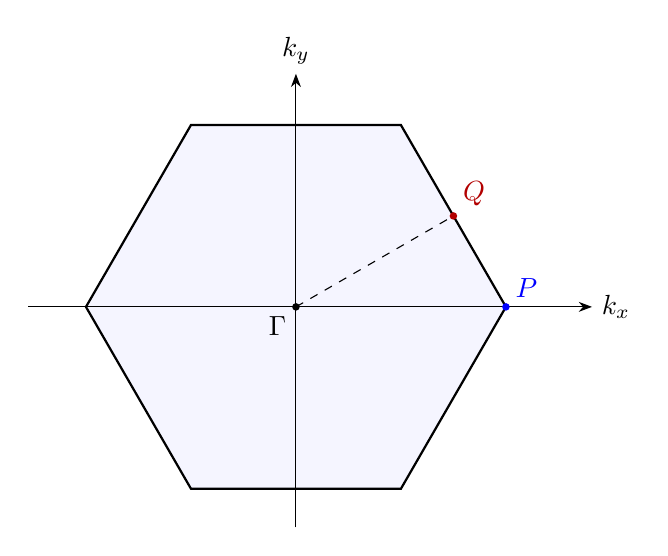
\begin{tikzpicture}[scale=4,>=Stealth]
\draw[thick,fill=blue!4] (0.666667,0)--(0.333333,0.57735)--(-0.333333,0.57735)--(-0.666667,0)--(-0.333333,-0.57735)--(0.333333,-0.57735)--cycle;
\draw[->] (-0.85,0)--(0.94,0) node[right] {$k_x$};
\draw[->] (0,-0.7)--(0,0.74) node[above] {$k_y$};
\fill (0,0) circle (0.012) node[below left] {$\Gamma$};
\fill[blue] (0.666667,0) circle (0.012) node[above right] {$P$};
\fill[red!70!black] (0.5,0.288675) circle (0.012) node[above right] {$Q$};
\draw[dashed] (0,0)--(0.5,0.288675);
\end{tikzpicture}

\small First Brillouin zone, in units of $2\pi/a$. The source's $P,Q$ are commonly called $K,M$.
\end{center}

\subsection*{(b) There is no gap}
The band separation is $E_+-E_-=2\gamma|F_{\vct k}|\geq0$ and vanishes at $P$ and symmetry-equivalent corners:
\[
\boxed{E_g=0.}
\]
At half filling with $E_F=E_p$, the Fermi surface reduces to Dirac points in this model.

\subsection*{(c) Choose the lower-band minimum at $\Gamma$}
Use DOS per area, per spin, for one local patch:
\[
D(E)=\int_{\rm patch}\frac{\dd^2q}{(2\pi)^2}\delta(E-E(\vct q)).
\]
Let $E_0=E_p-3\gamma$, $A=\gamma a^2/4$, and approximate $E=E_0+Aq^2$ in a circular patch $q<\Lambda$. Setting $z=Aq^2$ gives $q\dd q=\dd z/(2A)$:
\begin{align*}
D_\Gamma(E)&=\frac1{2\pi}\int_0^\Lambda q\dd q\,\delta(E-E_0-Aq^2)\\
&=\boxed{\frac1{\pi\gamma a^2}
\Theta(E-E_0)\Theta(E_0+A\Lambda^2-E).}
\end{align*}
The local approximation gives a constant step at the band edge; the upper cutoff depends on the patch. Multiply by two for both spins and by sample area $\mathcal A$ for a total DOS.

\paragraph{Additional check: the saddle at $Q$.}
For the upper band set $\varepsilon=E-(E_p+\gamma)$. With $\varepsilon=\alpha q_1^2-\eta q_2^2$, use $u=\sqrt\alpha q_1$, $v=\sqrt\eta q_2$, then $s=u+v$, $t=u-v$. Thus $u^2-v^2=st$ and $\dd u\dd v=\dd s\dd t/2$. For a local cutoff $|s|,|t|<L$,
\begin{align*}
D_Q(E)&\simeq\frac1{8\pi^2\sqrt{\alpha\eta}}
\int_{-L}^L\dd s\int_{-L}^L\dd t\,\delta(\varepsilon-st)\\
&=\frac1{4\pi^2\sqrt{\alpha\eta}}\ln\frac{L^2}{|\varepsilon|}\\
&=\frac1{\pi^2\sqrt3\gamma a^2}
\ln\frac{E_c}{|E-(E_p+\gamma)|}.
\end{align*}
This logarithmic van Hove divergence is per saddle and per spin. Its cutoff $E_c$ cannot be fixed by the quadratic expansion alone. In contrast, one Dirac valley gives
\[
D_P(E)=\frac{|E-E_p|}{2\pi\beta^2},\qquad\beta=\sqrt3\gamma a/2,
\]
which vanishes at the touching. These are three distinct DOS signatures.

\clearpage
\section*{Supplementary exercises from handwritten topics}
\begin{sourceNote}
The topics below are recognizable in attached handwritten answers, but their printed question statements, weights, and exact requested scope are missing. Exercises A--D are newly composed learning material, not verbatim reconstructions of original Questions 4--7.
\end{sourceNote}

\subsection*{A. Derive Bloch form from translation symmetry}
\textbf{Exercise.} For a Hamiltonian with Bravais translation symmetry, derive the quasiperiodicity of a simultaneous energy and translation eigenstate.

Define $(T_{\vct R}\psi)(\vct r)=\psi(\vct r+\vct R)$. Then $[H,T_{\vct R}]=0$ and $T_{\vct R}T_{\vct R'}=T_{\vct R+\vct R'}$. Choose a simultaneous eigenstate within each energy eigenspace:
\[
T_{\vct R}\psi=\lambda(\vct R)\psi.
\]
Translations are unitary, so $|\lambda|=1$. The group law imposes $\lambda(\vct R+\vct R')=\lambda(\vct R)\lambda(\vct R')$. Choose the primitive phases as $\lambda(\vct t_i)=\ee^{\ii\vct k\cdot\vct t_i}$; then
\[
\psi(\vct r+\vct R)=\ee^{\ii\vct k\cdot\vct R}\psi(\vct r).
\]
Defining $u_{\vct k}=\ee^{-\ii\vct k\cdot\vct r}\psi$ gives $u(\vct r+\vct R)=u(\vct r)$. Vectors $\vct k$ and $\vct k+\vct G$ have the same translation eigenvalues, so $\vct k$ may be chosen in the first Brillouin zone.

\subsection*{B. Brillouin's theorem and single excitations}
\textbf{Exercise.} Show that a self-consistent HF determinant has zero Hamiltonian matrix element with every singly excited determinant.

Let $\Phi_0$ be the stationary HF determinant and $\Phi_i^a$ replace occupied spin orbital $i$ by virtual orbital $a$. The Slater--Condon rules give
\[
\bra{\Phi_i^a}H\ket{\Phi_0}
=h_{ai}+\sum_{j\in\mathrm{occ}}
\bigl(\langle aj|v|ij\rangle-\langle aj|v|ji\rangle\bigr)=F_{ai}.
\]
For canonical orbitals, $F\chi_i=\epsilon_i\chi_i$ and $\braket{\chi_a}{\chi_i}=0$, hence
\[
\boxed{\bra{\Phi_i^a}H\ket{\Phi_0}=0.}
\]
Equivalently, varying the real and imaginary components of the orbital rotation $\chi_i\mapsto\chi_i+\theta\chi_a$ must give zero first-order energy change. The theorem removes only the coupling to single excitations; double-excitation couplings generally survive, so HF need not be exact.

\subsection*{C. A determinant is an exact noninteracting eigenstate}
\textbf{Exercise.} If $H_0=\sum_{j=1}^Nh(j)$ and $h\chi_i=\epsilon_i\chi_i$, show that the determinant has energy $\sum_i\epsilon_i$.

Expand the determinant:
\[
\Phi=\frac1{\sqrt{N!}}\sum_P(-1)^P\prod_{j=1}^N\chi_{P(j)}(x_j).
\]
For every permutation, $H_0$ acting on the product gives the same eigenvalue $\sum_j\epsilon_{P(j)}=\sum_i\epsilon_i$. Therefore
\[
H_0\Phi=\left(\sum_{i=1}^N\epsilon_i\right)\Phi.
\]
The ground state fills the lowest available $N$ spin orbitals. Adding a true two-body interaction invalidates this argument, which is why an exact noninteracting determinant must be distinguished from an interacting HF approximation.

\subsection*{D. Hartree, Hartree--Fock, and Kohn--Sham}
\textbf{Exercise.} Compare the single-particle equations, variational objects, and treatment of exchange and correlation.

Let $h=-\hbar^2\nabla^2/(2m_e)+v_{\rm ext}$ and $\kappa=e^2/(4\pi\epsilon_0)$.
\begin{enumerate}[label=(\roman*)]
\item \textbf{Hartree.} Vary a product $\prod_i\chi_i$:
\[
\left[h+\sum_{j\ne i}J_j\right]\chi_i=\epsilon_i\chi_i,\qquad
J_j(\vct r)=\int\frac{\kappa|\chi_j(x')|^2}{|\vct r-\vct r'|}\dd x'.
\]
It includes the other electrons' average Coulomb field but no antisymmetry-driven exchange.
\item \textbf{Hartree--Fock.} Vary a single determinant:
\[
\left[h+\sum_j(J_j-K_j)\right]\chi_i=\epsilon_i\chi_i,
\]
\[
(K_j\chi_i)(x)=\chi_j(x)\int
\frac{\kappa\chi_j^*(x')\chi_i(x')}{|\vct r-\vct r'|}\dd x'.
\]
Exchange is nonlocal and $J_i-K_i$ cancels self-interaction. Correlation beyond a single determinant is generally missing.
\item \textbf{Kohn--Sham.} Introduce auxiliary noninteracting orbitals reproducing the interacting density:
\[
F[n]=T_s[n]+E_H[n]+E_{xc}[n],\quad
E_H=\frac\kappa2\iint\frac{n(\vct r)n(\vct r')}{|\vct r-\vct r'|}\dd^3r\dd^3r'.
\]
Orbital variation gives
\[
[h+v_H(\vct r)+v_{xc}(\vct r)]\varphi_i=\epsilon_i\varphi_i,\qquad
n=\sum_i f_i|\varphi_i|^2,
\]
with spin summation understood, $v_H=\delta E_H/\delta n$, and $v_{xc}=\delta E_{xc}/\delta n$. The functional $E_{xc}$ contains both nonclassical interactions and the difference between true and auxiliary kinetic energies. It is not merely HF exchange renamed. An exact functional gives exact ground-state density and energy in principle; approximate functionals add their own errors.
\end{enumerate}

\section*{Primary references used for checks}
\href{https://journals.aps.org/pr/abstract/10.1103/PhysRev.136.B864}{P. Hohenberg and W. Kohn, Inhomogeneous Electron Gas, Phys. Rev. 136, B864 (1964)};
\href{https://journals.aps.org/pr/abstract/10.1103/PhysRev.140.A1133}{W. Kohn and L. J. Sham, Self-Consistent Equations Including Exchange and Correlation Effects, Phys. Rev. 140, A1133 (1965)}.
Exercises A--D are explicitly new exercises based on the note topics. The original printed continuation remains missing.

\chapter{Solutions: Midterm, 5 December 2014}
\label{s:theory-2014-12-midterm}
\begin{sourceNote}
All seven printed questions survive. Their weights total 110\% and are retained. The derivations below are independent of handwritten answers. In Question 2, $a$ is the conventional cubic lattice parameter; in Question 3 it is the two-dimensional primitive-translation length.
\end{sourceNote}

\section*{1. Eight definitions}
\begin{enumerate}[label=(\alph*)]
\item \textbf{Bravais lattice.}
A three-dimensional Bravais lattice is the point set
\[
\mathcal L=\{\vct R=n_1\vct t_1+n_2\vct t_2+n_3\vct t_3:n_i\in\mathbb Z\},
\]
with linearly independent primitive vectors. Every lattice point has the same environment under translation. A lattice describes translational symmetry; a lattice point need not represent one atom.
\item \textbf{Composite crystal.}
In the lattice-plus-basis terminology relevant here, attach the same atomic basis $\{(\vct d_\alpha,s_\alpha)\}$ to each Bravais point. Positions are $\vct R+\vct d_\alpha$, with $s_\alpha$ specifying species. Even identical atoms at different basis sites need not be related by a Bravais translation. The honeycomb crystal has a two-atom basis on a triangular Bravais lattice.
\item \textbf{Brillouin zone.}
The first Brillouin zone is the reciprocal origin's Wigner--Seitz cell:
\[
|\vct k|\leq|\vct k-\vct G|\quad\hbox{for every }\vct G\in\mathcal L^*.
\]
Its faces are perpendicular bisectors between the origin and other reciprocal points. Higher zones can be classified by the number of crossed Bragg planes.
\item \textbf{Reciprocal lattice.}
With $\vct t_i\cdot\vct g_j=2\pi\delta_{ij}$,
\[
\mathcal L^*=\{m_1\vct g_1+m_2\vct g_2+m_3\vct g_3:m_i\in\mathbb Z\}.
\]
Equivalently $\ee^{\ii\vct G\cdot\vct R}=1$ for every direct-lattice translation.
\item \textbf{Bloch theorem.}
For a single-particle Hamiltonian with lattice symmetry, eigenstates can be chosen as
\[
\psi_{n\vct k}(\vct r)=\ee^{\ii\vct k\cdot\vct r}u_{n\vct k}(\vct r),\quad
u_{n\vct k}(\vct r+\vct R)=u_{n\vct k}(\vct r).
\]
Thus $\psi(\vct r+\vct R)=\ee^{\ii\vct k\cdot\vct R}\psi(\vct r)$: $\psi$ is generally quasiperiodic, while $u$ is periodic. The theorem follows from simultaneous diagonalization of the Hamiltonian and commuting translations.
\item \textbf{Exchange energy.}
For a determinant of orthonormal spin orbitals $\chi_i(x)$, $x=(\vct r,\sigma)$,
\[
E_{ee}=\frac12\sum_{ij}(J_{ij}-K_{ij}),\qquad E_x=-\frac12\sum_{ij}K_{ij},
\]
\[
K_{ij}=\iint\chi_i^*(x)\chi_j^*(x')
\frac{\kappa\,\chi_j(x)\chi_i(x')}{|\vct r-\vct r'|}\dd x\dd x',
\qquad\kappa=\frac{e^2}{4\pi\epsilon_0}.
\]
Exchange arises from antisymmetry; separated spin functions restrict it to equal-spin pairs. It is not an additional classical force or the entire correlation energy.
\item \textbf{Fully spin-polarized ground state.}
All spins point in the same direction: $N_\uparrow=N$, $N_\downarrow=0$ gives $\zeta=(N_\uparrow-N_\downarrow)/N=1$, $S_z=N\hbar/2$, and total-spin quantum number $S=N/2$. It does not mean zero spin.
\item \textbf{Wigner crystallization.}
At sufficiently low density, an electron gas in a uniform positive background can form an ordered electron crystal. With mean spacing $r_sa_0$, kinetic and Coulomb scales vary as $r_s^{-2}$ and $r_s^{-1}$, respectively; interactions become relatively more important at large $r_s$. This is spontaneous density ordering, not merely drawing a Wigner--Seitz cell.
\end{enumerate}

\section*{2. Lattice planes and translation phase}
\subsection*{Reciprocal basis and primitive volume}
From $\vct g_1=2\pi(\vct t_2\times\vct t_3)/\Omega$ and cyclic permutations,
\[
\Omega=\vct t_1\cdot(\vct t_2\times\vct t_3)=\frac{a^3}{4},
\]
\[
\boxed{\vct g_1=\frac{2\pi}{a}(-1,1,1),\quad
\vct g_2=\frac{2\pi}{a}(1,-1,1),\quad
\vct g_3=\frac{2\pi}{a}(1,1,-1).}
\]
One point per primitive cell gives $\rho_3=4/a^3$. For coprime integers $h_i$, let $\vct G_0=\sum_i h_i\vct g_i$. At lattice points,
\[
\vct G_0\cdot\vct R=2\pi(h_1n_1+h_2n_2+h_3n_3)=2\pi m.
\]
Every integer $m$ occurs. Thus successive planes containing lattice points have
\[
\boxed{d=2\pi/|\vct G_0|.}
\]
Use the shortest reciprocal vector parallel to the specified normal; otherwise the level planes may include empty planes.

\subsection*{(a) Normal $3\vct g_1+6\vct g_2-6\vct g_3$}
Remove the common factor $3$:
\[
\vct G_0=\vct g_1+2\vct g_2-2\vct g_3
=\frac{2\pi}{a}(-1,-3,5),\qquad\gcd(1,2,-2)=1.
\]
Consequently
\[
\boxed{d=a/\sqrt{35}.}
\]
Directly using the printed normal's length would incorrectly divide this answer by three.

\subsection*{(b) Surface density}
A primitive planar cell of area $A_2$, stacked by a lattice translation with normal component $d$, gives $A_2d=\Omega$. Hence
\[
\boxed{\rho_2=\frac1{A_2}=\frac d\Omega=\frac4{a^2\sqrt{35}}.}
\]
For an explicit check, all integer solutions of $n_1+2n_2-2n_3=0$ are generated by
\[
\vct u=-2\vct t_1+\vct t_2=\frac a2(1,-2,-1),\qquad
\vct v=2\vct t_1+\vct t_3=\frac a2(1,3,2).
\]
Their cross-product magnitude is $A_2=a^2\sqrt{35}/4$.

\subsection*{(c) Normal $\tfrac12\vct t_1+\vct t_2-\vct t_3$}
The direction is $a(0,-1,3)/4$. A reciprocal vector has components
\[
\frac{2\pi}{a}(-h_1+h_2+h_3,\ h_1-h_2+h_3,\ h_1+h_2-h_3).
\]
Setting these equal to $(2\pi/a)(0,-\lambda,3\lambda)$ gives $(h_1,h_2,h_3)=(\lambda,3\lambda/2,-\lambda/2)$. The smallest positive $\lambda$ giving integer coefficients is $2$:
\[
\vct G_0=2\vct g_1+3\vct g_2-\vct g_3=\frac{2\pi}{a}(0,-2,6),
\qquad\boxed{d=a/\sqrt{40}.}
\]
The shorter vector $(2\pi/a)(0,-1,3)$ is not reciprocal: its primitive coefficients are half-integers.

\subsection*{(d) Periodicity}
For $f(\vct r)=\exp(\ii\vct g_1\cdot\vct r/2)$,
\[
f(\vct r+\vct t_1)=f(\vct r)\ee^{\ii\pi}=-f(\vct r).
\]
Thus \textbf{no}. The squared magnitude is uniform, but the complex wavefunction retains only translations with even $n_1$, not all periods of the original lattice.

\section*{3. Critical points and two-dimensional DOS}
Let $E_\pm=E_p\pm\gamma\sqrt S$, with
\[
S=1+4\cos x\cos y+4\cos^2x,\quad x=\frac{ak_x}{2},\quad y=\frac{\sqrt3ak_y}{2}.
\]
An ordinary stationary critical point is differentiable and satisfies $\nabla E=0$. At a touching, $\nabla S=0$ does not by itself imply $\nabla\sqrt S=0$.

\subsection*{(a) $\Gamma$ and $P$}
At $\Gamma$,
\[
S=9-6x^2-2y^2+O(k^4)=9-\frac32a^2k^2+O(k^4),
\]
\[
\sqrt S=3-\frac{a^2k^2}{4}+O(k^4),\qquad
E_\pm=E_p\pm3\gamma\mp\frac{\gamma a^2}{4}k^2+O(k^4).
\]
Hence $\Gamma$ is a maximum of the upper band and a minimum of the lower band. The Hessians $\mp(\gamma a^2/2)I$ are definite.

At $P=(4\pi/(3a),0)$, write $\vct k=\vct P+\vct q$. Then
\[
S=\frac34a^2(q_x^2+q_y^2)+O(q^3),\qquad
\boxed{E_\pm=E_p\pm\beta|\vct q|+O(q^2),\quad\beta=\frac{\sqrt3\gamma a}{2}.}
\]
Along $q_y=0$, the term $\beta|q_x|$ has unequal left and right derivatives. Therefore $P$ is a \textbf{Dirac touching, not a differentiable zero-gradient critical point}. A broader terminology may call it a nonsmooth upper-band minimum and lower-band maximum, but the conical nature must be stated; a quadratic effective-mass approximation is invalid.

\begin{center}
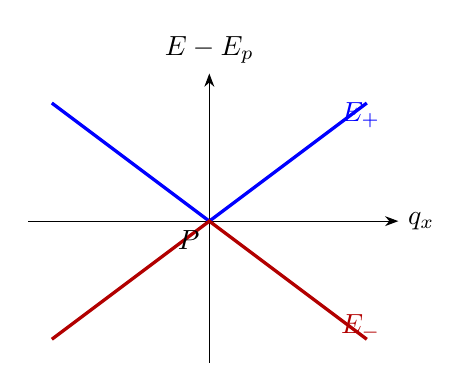
\begin{tikzpicture}[x=1cm,y=0.75cm,>=Stealth]
\draw[->] (-2.3,0)--(2.4,0) node[right] {$q_x$};
\draw[->] (0,-2.4)--(0,2.5) node[above] {$E-E_p$};
\draw[very thick,blue] (-2,2)--(0,0)--(2,2);
\draw[very thick,red!70!black] (-2,-2)--(0,0)--(2,-2);
\node[blue,right] at (1.55,1.8) {$E_+$};
\node[red!70!black,right] at (1.55,-1.8) {$E_-$};
\node[below left] at (0,0) {$P$};
\end{tikzpicture}

\small Section through a Dirac cone: opposite sides have different slopes.
\end{center}

\subsection*{(b) DOS around the lower-band minimum at $\Gamma$}
Define the DOS per real-space area, per spin, for one local patch:
\[
D(E)=\int_{\rm patch}\frac{\dd^2q}{(2\pi)^2}\delta(E-E(\vct q)).
\]
Let $E_0=E_p-3\gamma$, $\alpha=\gamma a^2/4$, and use $E=E_0+\alpha q^2$ in $q<\Lambda$. Then
\begin{align*}
D_-(E)&=\frac1{2\pi}\int_0^\Lambda q\,\dd q\,\delta(E-E_0-\alpha q^2)\\
&=\boxed{\frac1{4\pi\alpha}\Theta(E-E_0)\Theta(E_0+\alpha\Lambda^2-E)}\\
&=\frac1{\pi\gamma a^2}\Theta(E-E_0)\Theta(E_0+\alpha\Lambda^2-E).
\end{align*}
This is the constant step at a two-dimensional parabolic extremum. The upper-band maximum $E_1=E_p+3\gamma$ gives a reversed step with the same height for $E_1-\alpha\Lambda^2<E<E_1$. Multiply by sample area for total DOS and by two for both spins. No extra valley factor belongs to a single patch.

For comparison, one Dirac valley per spin gives
\[
D_P(E)=\frac{|E-E_p|}{2\pi\beta^2}=\frac{2|E-E_p|}{3\pi\gamma^2a^2},
\]
which vanishes at the touching energy.

\section*{4. Hamiltonian with fixed nuclei}
Fix nuclear coordinates $\vct R_A$ and charges $Z_Ae$. Neglect relativity, spin--orbit coupling, and nuclear motion. Define
\[
v_{\rm ext}(\vct r)=-\sum_A\frac{Z_A\kappa}{|\vct r-\vct R_A|},\qquad
h(i)=-\frac{\hbar^2}{2m_e}\nabla_i^2+v_{\rm ext}(\vct r_i).
\]
Then
\[
\boxed{H_e=\sum_{i=1}^Nh(i)+\sum_{i<j}\frac{\kappa}{r_{ij}}.}
\]
These terms are electron kinetic energy, nuclear attraction, and electron repulsion. Total energy at the fixed nuclear configuration also includes the constant
\[
E_{nn}=\sum_{A<B}\frac{Z_AZ_B\kappa}{|\vct R_A-\vct R_B|}.
\]
This does not affect electronic variation. Writing the pair sum as $\sum_{i\ne j}$ requires a factor $1/2$.

\section*{5. Hartree trial state}
For $x_i=(\vct r_i,\sigma_i)$,
\[
\boxed{\Psi_H(x_1,\ldots,x_N)=\prod_{i=1}^N\chi_i(x_i),\qquad
\int|\chi_i(x)|^2\dd x=1.}
\]
The expectation value is
\[
E_H=\sum_i h_{ii}+\frac12\sum_{i\ne j}J_{ij},\qquad
J_{ij}=\iint\frac{\kappa|\chi_i(x)|^2|\chi_j(x')|^2}{|\vct r-\vct r'|}\dd x\dd x'.
\]
Variation of each normalized orbital gives the average Hartree field of the other electrons. The product does not enforce antisymmetry, so it does not fully satisfy fermionic statistics and has no exchange term.

\section*{6. Hartree--Fock trial state and optimization}
\subsection*{Antisymmetrization and energy}
Take orthonormal spin orbitals:
\[
\boxed{\Psi_{\rm HF}(x_1,\ldots,x_N)=\frac1{\sqrt{N!}}\det[\chi_i(x_j)]_{i,j=1}^N,\quad
\braket{\chi_i}{\chi_j}=\delta_{ij}.}
\]
Exchanging two electron coordinates exchanges columns and changes the sign. Its energy is
\[
E_{\rm HF}=\sum_i h_{ii}+\frac12\sum_{ij}(J_{ij}-K_{ij}).
\]
Since $J_{ii}=K_{ii}$, self-interaction cancels.

\subsection*{Constrained variation}
Minimize
\[
\mathcal L=E_{\rm HF}-\sum_{ij}\lambda_{ij}
(\braket{\chi_i}{\chi_j}-\delta_{ij}).
\]
Variation with respect to $\chi_i^*(x)$ gives
\[
F\chi_i=\sum_j\lambda_{ij}\chi_j,\qquad F=h+\sum_{j\in\rm occ}(J_j-K_j),
\]
\begin{align*}
(J_jf)(x)&=\left[\int\frac{\kappa|\chi_j(x')|^2}{|\vct r-\vct r'|}\dd x'\right]f(x),\\
(K_jf)(x)&=\chi_j(x)\int\frac{\kappa\chi_j^*(x')f(x')}{|\vct r-\vct r'|}\dd x'.
\end{align*}
$J_j$ is local; $K_j$ is nonlocal. Diagonalize the Hermitian multiplier matrix by a unitary rotation of occupied orbitals, changing the determinant only by an overall phase. The canonical equations are
\[
\boxed{F\chi_i=\epsilon_i\chi_i.}
\]

\subsection*{Self-consistency and limitations}
Guess orbitals, build the density and Fock operator, solve its eigenproblem, occupy $N$ orbitals, and update until density and energy converge. Compare distinct spin or symmetry solutions; convergence alone does not prove the global minimum. The optimized determinant is a variational approximation in a restricted space, not generally an exact correlated state. Its total energy is
\[
E_{\rm HF}=\sum_i\epsilon_i-\frac12\sum_{ij}(J_{ij}-K_{ij}),
\]
not the uncorrected eigenvalue sum.

\section*{7. Slater--Jastrow trial state}
For a fluid electron gas in periodic volume $\Omega$, use momentum-state determinants times a positive pair-correlation factor:
\[
\boxed{\Psi_T(\vct R)=D_\uparrow D_\downarrow
\exp\left[-\sum_{i<j}u_{\sigma_i\sigma_j}(r_{ij})\right],\qquad
\vct R=(\vct r_1,\ldots,\vct r_N).}
\]
For example $D_\sigma=\det[\ee^{\ii\vct k_\alpha\cdot\vct r_j}/\sqrt\Omega]$ fills the chosen Fermi sea for each spin population. This is a fixed-spin coordinate component; the complete spin wavefunction remains antisymmetric. A fully polarized state has one spin determinant.

The determinants supply antisymmetry and nodes. The symmetric positive Jastrow factor preserves the nodes while changing pair probabilities and lowering correlation energy. Its short-range form can satisfy Coulomb cusp conditions; its long-range form can incorporate screening and collective fluctuations. Optimize its parameters variationally. A trial crystal phase can instead use localized orbitals around lattice sites.

Sampling $p(\vct R)\propto|\Psi_T(\vct R)|^2$ gives the local-energy average:
\[
E_T=\frac{\int|\Psi_T|^2E_L\,\dd\vct R}{\int|\Psi_T|^2\,\dd\vct R},\quad
E_L=\frac{H\Psi_T}{\Psi_T},\quad E_T\geq E_0.
\]
Projection Monte Carlo further filters higher energies with imaginary-time evolution $\ee^{-\tau(H-E_T)}$. Holding trial nodes fixed yields a fixed-node approximation, not an error-free exact result. The Ceperley--Alder stochastic projection study is more than a single variational sampling calculation.

\section*{Primary reference used for checks}
\href{https://journals.aps.org/prl/abstract/10.1103/PhysRevLett.45.566}{D. M. Ceperley and B. J. Alder, Ground State of the Electron Gas by a Stochastic Method, Phys. Rev. Lett. 45, 566 (1980)}.
An \href{https://people.physics.illinois.edu/Ceperley/papers/015.pdf}{author-hosted full text} is available. The lattice geometry, band expansions, DOS factors, and variational steps were derived independently.

\chapter{Solutions: Midterm Exam, April 30, 2015}
\label{s:physics-2015-04-midterm}
These solutions are derived from the stated assumptions. The density of states $D(E)$ counts states per unit energy in the entire volume $V$. The factor $g_s$ denotes any spin degeneracy included separately; the free-electron gas uses $g_s=2$ without double counting.

\section*{1. Lattice translations in BaTiO$_3$}
For the cubic model specified in the question, the Bravais translations are
$\vct R=a(n_x,n_y,n_z)$ with $n_i\in\mathbb Z$. A five-atom basis is
\[
\begin{array}{c|c}
\text{Atom}&\vct\tau/a\\ \hline
\mathrm{Ba}&(0,0,0)\\
\mathrm{Ti}&(1/2,1/2,1/2)\\
\mathrm{O}_1&(1/2,1/2,0)\\
\mathrm{O}_2&(1/2,0,1/2)\\
\mathrm{O}_3&(0,1/2,1/2)
\end{array}
\]
Actual atomic positions are $\vct R+\vct\tau_\nu$. A displacement is a Bravais translation precisely when it belongs to $a\mathbb Z^3$.
\begin{enumerate}[label=(\alph*)]
\item \textbf{True.} There is one Ti basis position in each primitive cell, so subtraction cancels the basis position:
\[
(\vct R_m+\vct\tau_{\rm Ti})-(\vct R_n+\vct\tau_{\rm Ti})=\vct R_m-\vct R_n.
\]
This is always a lattice translation.
\item \textbf{True.} A Ba-to-Ti displacement has the form
$a(n_x+1/2,n_y+1/2,n_z+1/2)$. Its half-integer components exclude it from $a\mathbb Z^3$.
\item \textbf{False.} Two O atoms with the same basis index are related by a translation, but the assertion concerns any two O atoms. Within one cell,
\[
\vct\tau_{\mathrm O_2}-\vct\tau_{\mathrm O_1}=\frac a2(0,-1,1),
\]
which is not a simple-cubic lattice translation. Having the same chemical species does not imply having the same basis index.
\end{enumerate}

\section*{2. The fcc lattice, its reciprocal lattice, and lattice planes}
\subsection*{(a) Primitive-cell volumes}
The given vectors are primitive vectors of a face-centered cubic (fcc) lattice. Their scalar triple product is
\[
\Omega=\abs{\vct t_1\cdot(\vct t_2\times\vct t_3)}
=\left(\frac a2\right)^3
\det\begin{pmatrix}0&1&1\\1&0&1\\1&1&0\end{pmatrix}
=\frac{a^3}{4}.
\]
A Wigner--Seitz cell is also a primitive cell. The reciprocal primitive-cell volume, equal to the first Brillouin-zone volume, is $(2\pi)^3/\Omega$. Thus
\[
\boxed{V_{\rm WS}=\frac{a^3}{4}},\qquad
\boxed{V_{\rm BZ}=\frac{32\pi^3}{a^3}}.
\]

\subsection*{(b) Reciprocal primitive vectors}
Using $\vct g_1=2\pi(\vct t_2\times\vct t_3)/\Omega$ and cyclic permutations gives
\[
\boxed{\vct g_1=\frac{2\pi}{a}(-1,1,1),\quad
\vct g_2=\frac{2\pi}{a}(1,-1,1),\quad
\vct g_3=\frac{2\pi}{a}(1,1,-1)}.
\]
For example, $\vct t_1\cdot\vct g_1=2\pi$ and
$\vct t_1\cdot\vct g_2=\vct t_1\cdot\vct g_3=0$. The other rows give the same reciprocal orthogonality relation.

\subsection*{(c) Spacing of successive occupied lattice planes}
The unit normal is $\hat{\vct n}=(0,1,1)/\sqrt2$. Project an arbitrary lattice point
$\vct R=n_1\vct t_1+n_2\vct t_2+n_3\vct t_3$ onto this direction:
\[
\hat{\vct n}\cdot\vct R
=\frac{a}{2\sqrt2}(2n_1+n_2+n_3).
\]
The integer in parentheses can take every integer value. Successive planes containing fcc lattice points therefore lie at
$\hat{\vct n}\cdot\vct R=j a/(2\sqrt2)$, giving
\[
\boxed{d=\frac{a}{2\sqrt2}}.
\]
Equivalently, the shortest nonzero reciprocal vector parallel to the normal is
$\vct G=2\vct g_1+\vct g_2+\vct g_3=(4\pi/a)(0,1,1)$, and $d=2\pi/|\vct G|$.
\begin{sourceNote}
Here ``successive lattice planes'' means successive occupied fcc layers. The formal conventional-cubic $(011)$ spacing is $a/\sqrt2$, but fcc centering supplies an additional occupied layer halfway between those planes. The occupied-layer spacing requested under this interpretation is consequently half as large.
\end{sourceNote}

\subsection*{(d) Areal density}
Two perpendicular in-plane translations are
\[
\vct u=a(1,0,0)=-\vct t_1+\vct t_2+\vct t_3,\qquad
\vct v=\frac a2(0,1,-1)=\vct t_3-\vct t_2.
\]
They generate the two-dimensional lattice on this plane. Its primitive area is
$A_{\parallel}=|\vct u\times\vct v|=a^2/\sqrt2$, with one lattice point per primitive parallelogram. Hence
\[
\boxed{\sigma=\frac1{A_{\parallel}}=\frac{\sqrt2}{a^2}}.
\]
The volume check is $A_{\parallel}d=\Omega$, equivalently $\sigma=d/\Omega$.
\begin{center}
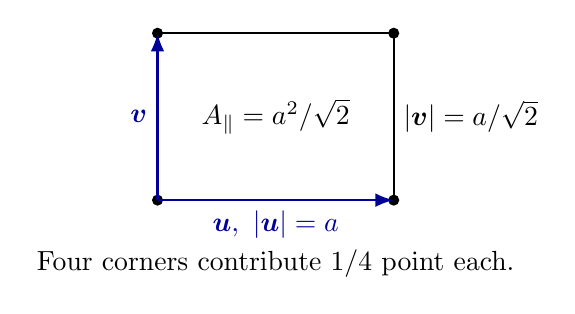
\begin{tikzpicture}[>=Latex]
\draw[thick] (0,0) rectangle (3,2.12);
\foreach \x in {0,3}\foreach \y in {0,2.12}\fill (\x,\y) circle (2pt);
\draw[->,blue!60!black,thick] (0,0)--(3,0) node[midway,below] {$\vct u,\ |\vct u|=a$};
\draw[->,blue!60!black,thick] (0,0)--(0,2.12) node[midway,left] {$\vct v$};
\node[right] at (3,1.06) {$|\vct v|=a/\sqrt2$};
\node at (1.5,1.06) {$A_{\parallel}=a^2/\sqrt2$};
\node[below] at (1.5,-.5) {Four corners contribute $1/4$ point each.};
\end{tikzpicture}
\end{center}

\subsection*{(e) Testing the proposed vectors}
Every reciprocal vector must satisfy
$\vct t_i\cdot\vct G\in2\pi\mathbb Z$ for all primitive translations. However,
\[
\vct t_1\cdot\vct G_1
=\frac a2(0,1,1)\cdot\frac\pi a(0,1,1)=\pi.
\]
Thus $\vct G_1$ is not even a reciprocal-lattice vector. The proposed vectors \textbf{do not} generate the required reciprocal lattice by integer linear combinations. Linear independence over the real numbers only guarantees that three vectors span three-dimensional vector space; it does not establish equality of discrete lattices.

\section*{3. Atomic density of diamond}
Diamond consists of an fcc Bravais lattice with a two-atom basis. A conventional cubic cell contains
$8(1/8)+6(1/2)=4$ fcc lattice points. With two atoms per point,
\[
\boxed{n_{\rm atom}=\frac{4\times2}{a^3}=\frac8{a^3}}.
\]
The equivalent primitive-cell count is two atoms divided by $a^3/4$.

\section*{4. Definitions}
\begin{enumerate}[label=(\alph*)]
\item \textbf{Three-dimensional hexagonal lattice.} One choice of primitive vectors is
\[
\vct a_1=a(1,0,0),\quad
\vct a_2=a(-1/2,\sqrt3/2,0),\quad
\vct a_3=c(0,0,1).
\]
The first two vectors have equal lengths and enclose $120^\circ$; the third is perpendicular to their plane. Their integer combinations define the hexagonal Bravais lattice, of primitive volume $\sqrt3a^2c/2$. Hexagonal close packing (hcp) adds a two-atom basis to this lattice; the lattice and its basis are separate concepts.
\item \textbf{Bloch theorem.} If a single-electron Hamiltonian is invariant under every lattice translation, its energy eigenstates can be chosen as
\[
\psi_{n\vct k}(\vct r)=\ee^{\ii\vct k\cdot\vct r}u_{n\vct k}(\vct r),
\qquad u_{n\vct k}(\vct r+\vct R)=u_{n\vct k}(\vct r).
\]
Equivalently,
$\psi_{n\vct k}(\vct r+\vct R)=\ee^{\ii\vct k\cdot\vct R}\psi_{n\vct k}(\vct r)$.
The wave vector labels crystal momentum and can be restricted to the first Brillouin zone modulo a reciprocal vector.
\item \textbf{Critical point.} A point where $\nabla_{\vct k}\varepsilon_n=0$. For a nondegenerate Hessian in three dimensions, the type $M_j$ counts its negative eigenvalues: $M_0$ is a minimum, $M_1$ and $M_2$ are saddles with one and two negative directions, and $M_3$ is a maximum.
\item \textbf{Fermi energy.} The highest occupied single-particle energy after filling the zero-temperature ground state at fixed particle number. For the free-electron gas here it equals $\mu(0)=\varepsilon_F$. Its energy reference must be specified; it is distinct from the work function required to remove an electron to vacuum.
\end{enumerate}

\section*{5. Density of states near a three-dimensional $M_1$ saddle}
\subsection*{(a) Local dispersion}
Set $\vct q=\vct k-\vct k_1$ and diagonalize the Hessian. The gradient vanishes at the critical point, so no linear term remains. With one negative-curvature direction,
\[
\boxed{\varepsilon(\vct k)
=\varepsilon_1+Aq_x^2+Bq_y^2-Cq_z^2+O(q^3)},
\qquad A,B,C>0.
\]
The coefficients $A,B,C$ already incorporate the factor $1/2$ in the Taylor expansion.

\subsection*{(b) Deriving the nonanalytic contribution with a local cutoff}
Define $X=\sqrt A q_x$, $Y=\sqrt B q_y$, $Z=\sqrt C q_z$, and $\Delta=E-\varepsilon_1$. Then
\[
D_{\rm loc}(E)=\frac{g_sV}{(2\pi)^3\sqrt{ABC}}
\int\dd X\dd Y\dd Z\,
\delta(\Delta-X^2-Y^2+Z^2).
\]
The quadratic saddle cannot be extended to infinity: its constant-energy surfaces are unbounded. Restrict it to a neighborhood, for example $|Z|<\Lambda$, with a transverse cutoff large enough to contain the relevant energy shells in the range considered. Polar integration over $X,Y$ gives
\[
\int_0^{\infty}2\pi\rho\dd\rho\,
\delta(\Delta+Z^2-\rho^2)=\pi\Theta(\Delta+Z^2).
\]
For $\Delta>0$, every $Z$ in $(-\Lambda,\Lambda)$ contributes. For
$-\Lambda^2<\Delta<0$, the interval $|Z|<\sqrt{-\Delta}$ has no real transverse radius and must be removed. Therefore
\[
D_{\rm loc}(E)=\frac{g_sV}{4\pi^2\sqrt{ABC}}
\left[\Lambda-\sqrt{\varepsilon_1-E}\,
\Theta(\varepsilon_1-E)\right].
\]
Other cutoff choices and other parts of the band change the regular background, while the leading local nonanalytic term is
\[
\boxed{D(E)=D_{\rm reg}(E)
-\frac{g_sV}{4\pi^2\sqrt{ABC}}
\sqrt{\varepsilon_1-E}\,\Theta(\varepsilon_1-E)}.
\]
This expression gives the leading behavior near the critical energy; higher-order terms in the dispersion can add subleading corrections. The density of states remains finite at $E=\varepsilon_1$, but its slope diverges on the lower-energy side. Local curvature alone cannot fix the absolute background $D_{\rm reg}$ of the whole band.
\begin{center}
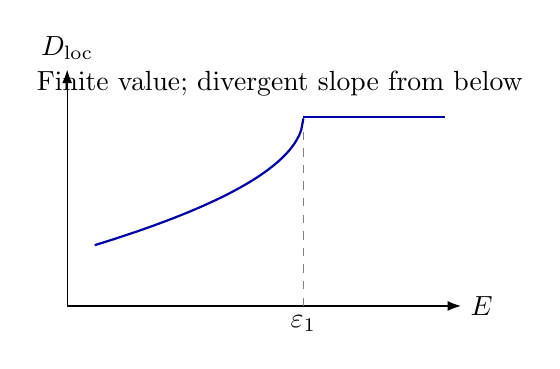
\begin{tikzpicture}[>=Latex]
\draw[->] (0,0)--(5,0) node[right] {$E$};
\draw[->] (0,0)--(0,3) node[above] {$D_{\rm loc}$};
\draw[dashed,gray] (3,0)--(3,2.4);
\draw[thick,blue!65!black,domain=.35:3,samples=100] plot (\x,{2.4-sqrt(3-\x)});
\draw[thick,blue!65!black] (3,2.4)--(4.8,2.4);
\node[below] at (3,0) {$\varepsilon_1$};
\node[above] at (2.7,2.55) {Finite value; divergent slope from below};
\end{tikzpicture}
\end{center}

\section*{6. Free-electron ground-state quantities in terms of $r_s$}
Let $a_0=4\pi\varepsilon_0\hbar^2/(m_e e^2)$ be the Bohr radius. By definition, a sphere of radius $r_sa_0$ contains the mean volume per electron:
\[
\frac1n=\frac{4\pi}{3}(r_sa_0)^3
\quad\Longrightarrow\quad
\boxed{n=\frac{3}{4\pi r_s^3a_0^3}}.
\]
Counting both spins inside the Fermi sphere gives
\[
N=2\frac V{(2\pi)^3}\frac{4\pi}{3}k_F^3,
\qquad n=\frac{k_F^3}{3\pi^2}.
\]
Consequently,
\begin{align*}
\boxed{k_F=\frac{(9\pi/4)^{1/3}}{r_sa_0}},\qquad
\boxed{\varepsilon_F=\frac{\hbar^2}{2m_ea_0^2}
\left(\frac{9\pi}{4}\right)^{2/3}\frac1{r_s^2}},\\
\boxed{T_F=\frac{\varepsilon_F}{\kb}}.
\end{align*}
The mean energy averages all occupied states, rather than only states on the Fermi surface:
\[
\overline\varepsilon
=\frac{\int_0^{k_F}(\hbar^2k^2/2m_e)k^2\dd k}
{\int_0^{k_F}k^2\dd k}
=\boxed{\frac35\varepsilon_F}.
\]

\section*{7. Low-temperature heat capacity and the printed coefficient}
For $T\ll T_F$, states well below the Fermi energy are almost completely filled. Pauli exclusion prevents arbitrary changes of their occupations. Thermal excitations predominantly involve an energy window of width of order $\kb T$ near $\varepsilon_F$.
Since $D(\varepsilon_F)=3N/(2\varepsilon_F)$ in three dimensions, the number of thermally active states scales as
\[
N_{\rm active}\sim D(\varepsilon_F)\kb T
=\frac32N\frac{T}{T_F}.
\]
Assigning a heat-capacity scale $\kb$ to each active state gives the estimate printed in the question: a suppression by $T/T_F$ relative to the classical value.

The printed factor $3/2$ is not the exact low-temperature coefficient. The Sommerfeld expansion at fixed $N,V$ gives
\[
C_V=\frac{\pi^2}{3}\kb^2T D(\varepsilon_F)
=\boxed{\frac{\pi^2}{2}N\kb\frac{T}{T_F}}
+O\!\left(N\kb(T/T_F)^3\right).
\]
Thus the physical argument establishes linear temperature dependence and a restricted thermally active population. It must not be interpreted as an exact derivation of the numerical coefficient $3/2$.

\section*{8. The exponential tail above the vacuum level}
The Fermi--Dirac distribution is
\[
f(E)=\frac1{\ee^{(E-\mu)/(\kb T)}+1}.
\]
Define the work function $\Phi=E_{\rm vac}-\mu>0$. When $\Phi\gg\kb T$, as in the usual low-temperature metallic regime, all $E\ge E_{\rm vac}$ satisfy
$x=(E-\mu)/(\kb T)\ge\Phi/(\kb T)\gg1$. It follows that
\[
f(E)=\frac{\ee^{-x}}{1+\ee^{-x}}
\simeq\boxed{\exp[-(E-\mu)/(\kb T)]}.
\]
The relative error of $f_{\rm exp}=\ee^{-x}$ is exactly
\[
\frac{f_{\rm exp}-f}{f}=\ee^{-x}
\le\ee^{-\Phi/(\kb T)}.
\]
The approximation is controlled by the energy separation from the chemical potential compared with thermal energy, not by the word ``vacuum'' alone.

\section*{References and checks}
The counting arguments and integrals are derived above. Primary teaching references for comparison are
\href{https://www.damtp.cam.ac.uk/user/tong/statphys/statmechhtml/S3.html}{David Tong, Statistical Physics, Chapter 3}
(state counting and the Sommerfeld expansion), and
\href{https://www.mit.edu/course/6/6.732/www/6.732-pt2.pdf}{M. S. Dresselhaus, MIT Solid State Physics Part II, Chapter 4}
(critical-point classification and the three-dimensional saddle-point singularity).

\chapter{Solutions: Final Exam, June 25, 2015}
\label{s:physics-2015-06-final}
The electronic and vibrational conventions are stated explicitly below. In particular, a band is counted before separately resolving spin unless otherwise specified, and phonon polarization vectors are mass-weighted as in the hint.

\section*{1. Bloch sums and their role in tight binding}
Let $\phi_{\nu a}(\vct r-\vct R-\vct\tau_\nu)$ be a localized orbital of type $a$ on basis atom $\nu$ in the cell at $\vct R$. For $N$ cells with periodic boundary conditions, define
\[
\boxed{\Phi_{\nu a,\vct k}(\vct r)
=\frac1{\sqrt N}\sum_{\vct R}\ee^{\ii\vct k\cdot\vct R}
\phi_{\nu a}(\vct r-\vct R-\vct\tau_\nu)}.
\]
The factor $N^{-1/2}$ is conventional; if orbitals on different sites overlap, the overlap matrix still determines the final normalization.

For any Bravais translation $\vct T$, reindex the sum by $\vct R'=\vct R-\vct T$:
\begin{align*}
\Phi_{\nu a,\vct k}(\vct r+\vct T)
&=\frac1{\sqrt N}\sum_{\vct R'}
\ee^{\ii\vct k\cdot(\vct R'+\vct T)}
\phi_{\nu a}(\vct r-\vct R'-\vct\tau_\nu)\\
&=\ee^{\ii\vct k\cdot\vct T}\Phi_{\nu a,\vct k}(\vct r).
\end{align*}
The sum therefore has precisely the Bloch translation property.

In tight binding, these symmetry-adapted localized-orbital sums form the basis at each wave vector:
\[
\psi_{n\vct k}=\sum_{\nu a}c_{\nu a}^{(n)}(\vct k)\Phi_{\nu a,\vct k}.
\]
Projecting the Schr\"odinger equation onto this basis gives
\[
\boxed{H(\vct k)c_n=E_n(\vct k)S(\vct k)c_n},
\]
where $H_{ij}=\langle\Phi_i|\hat H|\Phi_j\rangle$ and
$S_{ij}=\langle\Phi_i|\Phi_j\rangle$. In an orthonormal model, $S=I$.
Translational symmetry has reduced an extensive real-space problem to a finite matrix at each $\vct k$; hopping between localized orbitals determines the matrix entries and their wave-vector-dependent phases.

\section*{2. Five orbitals per Si atom and the band count}
For electrical and bonding properties, retain the valence $3s$ and three $3p$ orbitals. A useful fifth orbital is an excited effective $s$-like orbital $s^*$, giving the conventional
\[
\boxed{\{3s,3p_x,3p_y,3p_z,s^*\}\quad(sp^3s^*)}
\]
basis. The $s^*$ orbital improves the description of conduction bands; in an empirical model it is an effective excited orbital, not a claim that the isolated atom already occupies a fifth valence orbital. The filled $1s$, $2s$, and $2p$ shells are treated as core states for this low-energy model. The original model is described by
\href{https://www.sciencedirect.com/science/article/pii/0022369783900641}{Vogl, Hjalmarson, and Dow (1983)}.

Silicon has two atoms per diamond primitive cell. Five orbital functions per atom therefore yield
\[
\boxed{2\times5=10\ \text{bands before explicit spin resolution}}.
\]
Each atom supplies four valence electrons, so each primitive cell supplies eight. A filled band accommodates two electrons per primitive cell when both spins are included. Hence
\[
\boxed{\frac{2\times4}{2}=4\ \text{fully occupied valence bands}}.
\]
The other six bands of this model are unoccupied in the undoped ground state. If spin is represented explicitly, the matrix has dimension twenty and eight spin-resolved bands are occupied. These conventions are consistent with the
\href{https://www.nextnano.com/docu/nextnano3/tutorials/1D_TightBinding_bulk.html}{nextnano implementation of the $sp^3s^*$ model}.

\section*{3. Why a direct all-electron plane-wave expansion is expensive}
At fixed $\vct k$, a Bloch wave can be expanded as
\[
\psi_{n\vct k}(\vct r)=\sum_{\vct G}c_{n\vct k}(\vct G)
\ee^{\ii(\vct k+\vct G)\cdot\vct r}.
\]
Near a nucleus, the all-electron potential varies strongly and the wavefunctions contain short spatial scales. Valence functions must also remain orthogonal to localized core states, producing nodes and rapid core-region variation. Resolving a length scale $\ell$ requires components with $|\vct k+\vct G|$ of order $1/\ell$. A kinetic-energy cutoff
\[
\frac{\hbar^2|\vct k+\vct G|^2}{2m_e}\le E_{\rm cut}
\]
then requires a very large $E_{\rm cut}$ and many plane waves, even if only valence energies are sought. The basis is valid, but direct all-electron convergence can be inefficient.

One remedy is to replace the core-region problem by a pseudopotential with smooth pseudo-valence functions. Alternatively, augmented-plane-wave or projector-augmented-wave approaches retain or reconstruct atomic core-region structure while using smoother representations elsewhere. Orthogonalized-plane-wave methods also account explicitly for the core orthogonality constraint. In each case, the objective is to represent the sharp atomic behavior without forcing a uniform plane-wave basis to resolve every core length scale directly.

\section*{4. Pseudopotentials and smooth pseudo-wavefunctions}
A pseudopotential is an effective electron--ion operator replacing the explicit nuclear attraction and core-electron effects in a valence calculation. It is constructed to reproduce relevant valence eigenvalues and scattering behavior outside a chosen core region. It can be angular-momentum dependent and nonlocal; it need not be a single scalar function of position.

A pseudo-wavefunction follows the required valence behavior outside the core but replaces the rapid all-electron oscillations inside it by a smoother function. Its large-$|\vct G|$ Fourier coefficients are therefore much smaller. A substantially lower plane-wave cutoff can represent it to a chosen accuracy.

This is an approximation with a chosen core--valence partition and transferability range. Smoothness does not itself guarantee correct bonding in every environment, and the cutoff must still be converged. Practical construction and validation requirements are discussed in
\href{https://www.quantum-espresso.org/wp-content/uploads/2022/03/pseudo-gen.pdf}{Quantum ESPRESSO, Notes on pseudopotential generation}.

\section*{5. The adiabatic energy surface}
Collect all nuclear positions into $\vct R$ and the electronic coordinates into $\vct r$. For fixed nuclei, solve the electronic eigenproblem
\[
\hat H_e(\vct R)\Psi_n(\vct r;\vct R)
=\mathcal E_n(\vct R)\Psi_n(\vct r;\vct R).
\]
The adiabatic potential-energy surface for nuclear motion is
\[
\boxed{E_n(\vct R)=\mathcal E_n(\vct R)+V_{NN}(\vct R)},
\]
where $V_{NN}$ is the nucleus--nucleus repulsion. If that term has already been included in $\hat H_e$, it must not be added a second time.

The electronic eigenproblem is solved parametrically as the nuclei move. In the Born--Oppenheimer approximation, nuclei move on a selected surface, neglecting transitions to other electronic surfaces and the associated nonadiabatic couplings. Nuclear kinetic energy is not part of this potential-energy surface. Its gradient determines the forces, and its Hessian determines harmonic restoring forces about equilibrium.

\section*{6. Obtaining lattice normal modes from the ground surface}
\subsection*{Equilibrium and harmonic force constants}
First locate a stationary nuclear configuration $\vct R^0$ with
$\partial E_0/\partial R_{i\alpha}=0$. Let
$u_{i\alpha}=R_{i\alpha}-R^0_{i\alpha}$, where $i$ labels atoms and $\alpha$ labels Cartesian components. Expand
\[
E_0(\vct R^0+\vct u)=E_0(\vct R^0)
+\frac12\sum_{i\alpha,j\beta}\Phi_{i\alpha,j\beta}
 u_{i\alpha}u_{j\beta}+O(u^3),
\qquad
\Phi_{i\alpha,j\beta}
=\left.\frac{\partial^2E_0}{\partial R_{i\alpha}\partial R_{j\beta}}\right|_{\vct R^0}.
\]
The linear term vanishes at equilibrium. The Hessian is the harmonic force-constant matrix, obtained analytically or by converged finite differences of energies or forces.

\subsection*{Mass weighting and the eigenproblem}
Newton's equations in the harmonic approximation are
\[
M_i\ddot u_{i\alpha}=-\sum_{j\beta}\Phi_{i\alpha,j\beta}u_{j\beta}.
\]
Substitute $u_{i\alpha}(t)=A_{i\alpha}\ee^{-\ii\omega t}/\sqrt{M_i}$. This gives
\[
\sum_{j\beta}\mathcal D_{i\alpha,j\beta}A_{j\beta}=\omega^2 A_{i\alpha},
\qquad
\boxed{\mathcal D_{i\alpha,j\beta}
=\frac{\Phi_{i\alpha,j\beta}}{\sqrt{M_iM_j}}}.
\]
Diagonalizing the real-space mass-weighted Hessian yields the squared normal-mode frequencies and orthonormal polarization vectors. The physical displacements are obtained by dividing each atomic block of an eigenvector by $\sqrt{M_i}$.

\subsection*{Periodic crystal and stability}
For a periodic crystal with $r$ atoms per primitive cell, Fourier transformation block-diagonalizes the problem into a $3r\times3r$ dynamical matrix at each allowed $\vct q$. The next answer gives its entries. The branches $\omega_p(\vct q)$ and their eigenvectors are the lattice normal modes.

Translational invariance imposes the acoustic sum rule
\[
\sum_j\Phi_{i\alpha,j\beta}=0
\]
for every $i,\alpha,\beta$. Thus three rigid translations have zero frequency at $\vct q=0$. A mechanically stable harmonic equilibrium has no negative $\omega^2$; negative eigenvalues describe an instability rather than ordinary oscillations. A nondegenerate, well-separated \emph{electronic} ground surface justifies the adiabatic treatment but does not by itself prove that a chosen nuclear configuration is a local minimum.

\section*{7. Dynamical-matrix elements and phase convention}
To remove a notational ambiguity, use the symbol $D$ exactly as in the question for the force constants, and $\mathcal D$ for the mass-weighted dynamical matrix. Adopt
\[
D_{\nu\alpha,\nu'\alpha'}(\vct t_n)
=\left.\frac{\partial^2E_0}
{\partial u_{0\nu\alpha}\,\partial u_{n\nu'\alpha'}}\right|_0.
\]
Choose the displacement convention
\[
u_{n\nu\alpha}(t)=\frac{A_{\nu\alpha}(\vct q)}{\sqrt{M_\nu}}
\ee^{\ii\vct q\cdot\vct t_n-\ii\omega t}.
\]
Inserting this into the equation of motion for atom $(0,\nu)$ gives
\[
\boxed{\mathcal D_{\nu\alpha,\nu'\alpha'}(\vct q)
=\frac1{\sqrt{M_\nu M_{\nu'}}}
\sum_n D_{\nu\alpha,\nu'\alpha'}(\vct t_n)
\ee^{\ii\vct q\cdot\vct t_n}},
\]
and the eigenproblem
\[
\sum_{\nu'\alpha'}\mathcal D_{\nu\alpha,\nu'\alpha'}(\vct q)
A_{\nu'\alpha'}=\omega^2 A_{\nu\alpha}.
\]
Hessian symmetry and translation invariance give
$D_{\nu\alpha,\nu'\alpha'}(\vct t_n)
=D_{\nu'\alpha',\nu\alpha}(-\vct t_n)$, so $\mathcal D(\vct q)$ is Hermitian.

If the plane-wave factor is instead defined using the full equilibrium position
$\vct t_n+\vct\tau_\nu$, the exponential in the boxed matrix becomes
$\ee^{\ii\vct q\cdot(\vct t_n+\vct\tau_{\nu'}-\vct\tau_\nu)}$.
The two matrices are related by a diagonal unitary change of basis and have identical frequencies. Stating the convention prevents an apparent phase disagreement from becoming a physical one.

\section*{8. Counting BaTiO$_3$ vibrational degrees of freedom}
There are $r=5$ atoms per cell and three displacement coordinates per atom.
\begin{enumerate}[label=(\alph*)]
\item At each $\vct q$, the Fourier-space dynamical matrix acts on $3r=15$ coordinates, so its dimension is
\[
\boxed{15\times15}.
\]
If ``dynamical matrix'' instead refers to the complete real-space system of $N$ cells, its dimension is $15N\times15N$. The standard band/branch formulation uses the first convention.
\item There are $N$ allowed wave vectors and fifteen modes at each one:
\[
\boxed{15N\ \text{normal modes}}.
\]
The real-displacement condition relates complex amplitudes at $\vct q$ and $-\vct q$; it does not halve the total number of real mechanical degrees of freedom.
\item The three rigid translations evolve into three acoustic branches:
\[
\boxed{3\ \text{acoustic branches}}.
\]
\item The remaining branches are optical:
\[
\boxed{3r-3=12\ \text{optical branches}}.
\]
Each branch contains $N$ normal modes, so the corresponding mode counts are $3N$ acoustic and $12N$ optical.
\end{enumerate}

\section*{9. Long-wavelength optical polarization vectors}
The hint uses \emph{mass-weighted} vectors $\vct A_\nu$, not the actual atomic displacements. At $\vct q=0$, a rigid translation in direction $\hat{\vct e}_\alpha$ has a mass-weighted eigenvector proportional to
\[
\left(\sqrt{M_1}\hat{\vct e}_\alpha,
      \sqrt{M_2}\hat{\vct e}_\alpha\right).
\]
A finite-frequency optical eigenvector of the Hermitian dynamical matrix is orthogonal to each of the three zero-frequency translational vectors. Component by component this implies
\[
\sqrt{M_1}\vct A_1+\sqrt{M_2}\vct A_2=0,
\qquad
\vct A_2=-\sqrt{\frac{M_1}{M_2}}\vct A_1.
\]
Therefore
\[
\vct A_1^*\cdot\vct A_2
=-\sqrt{\frac{M_1}{M_2}}\abs{\vct A_1}^2,
\qquad
\boxed{\frac{\abs{\vct A_1}^2}{\vct A_1^*\cdot\vct A_2}
=-\sqrt{\frac{M_2}{M_1}}}.
\]
The result is unchanged by a common complex phase of the mode. In terms of the \emph{physical} displacement amplitudes $\vct u_\nu=\vct A_\nu/\sqrt{M_\nu}$, the corresponding relation is
\[
\vct u_2=-\frac{M_1}{M_2}\vct u_1,
\qquad M_1\vct u_1+M_2\vct u_2=0.
\]
The unit-cell center of mass is stationary in the optical limit. The square-root mass ratio in the requested answer arises specifically from the mass-weighted convention in the hint.

\begin{center}
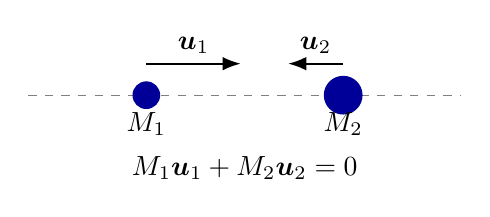
\begin{tikzpicture}[>=Latex]
\draw[gray,dashed] (-.5,0)--(5,0);
\fill[blue!60!black] (1,0) circle (5pt);
\fill[blue!60!black] (3.5,0) circle (7pt);
\draw[->,thick] (1,.4)--(2.2,.4) node[midway,above] {$\vct u_1$};
\draw[->,thick] (3.5,.4)--(2.8,.4) node[midway,above] {$\vct u_2$};
\node[below] at (1,-.1) {$M_1$};
\node[below] at (3.5,-.1) {$M_2$};
\node[below] at (2.25,-.65) {$M_1\vct u_1+M_2\vct u_2=0$};
\end{tikzpicture}
\end{center}
The schematic shows opposite motion; arrow lengths are illustrative. At an exactly soft optical instability, the optical subspace must be selected orthogonally to translations before taking the zero-frequency limit. The standard finite-frequency optical limit is assumed in the question.

\section*{References and checks}
The preceding formulas follow from the displayed translation, state-counting, and Hessian arguments. The primary sources used to check conventions are:
\begin{itemize}
\item \href{https://www.sciencedirect.com/science/article/pii/0022369783900641}{P. Vogl, H. P. Hjalmarson, and J. D. Dow, A Semi-empirical tight-binding theory of the electronic structure of semiconductors (1983)}: the $sp^3s^*$ basis.
\item \href{https://www.nextnano.com/docu/nextnano3/tutorials/1D_TightBinding_bulk.html}{nextnano, Empirical tight-binding $sp^3s^*$ band structure}: ten-orbital and twenty-spin-orbital matrix conventions.
\item \href{https://www.quantum-espresso.org/wp-content/uploads/2022/03/pseudo-gen.pdf}{Quantum ESPRESSO, Notes on pseudopotential generation}: effective-core construction and validation.
\item \href{https://www.quantum-espresso.org/Doc/INPUT_DYNMAT.html}{Quantum ESPRESSO, dynmat.x documentation}: orthogonal dynamical-matrix eigenvectors versus physical displacements divided by square roots of masses.
\item \href{https://davidtong.org/pdfs/teaching/solid-state-physics/solidstate4.pdf}{David Tong, Solid State Physics, Chapter 4}: lattice vibrations and acoustic/optical branches.
\end{itemize}

\chapter{Solutions: Midterm, 29 April 2016}
\label{s:theory-2016-04-midterm}
\begin{sourceNote}
All twelve printed questions are available. The solutions below distinguish exact statements from approximations and make the assumptions behind the true/false questions explicit. In Questions 7--10, $\psi$ always denotes the physical crystal state and $\varphi$ its auxiliary pseudo wavefunction; reversing these symbols reverses the projection relation.
\end{sourceNote}

\section*{1. True or false}
\subsection*{(a) A self-consistent HF determinant is an exact interacting eigenstate: false}
Hartree--Fock minimizes the expectation value of the interacting Hamiltonian within the set of single Slater determinants:
\[
E_{\rm HF}=\min_{\Phi\ {\rm determinant}}\frac{\bra\Phi H\ket\Phi}{\braket\Phi\Phi}
\geq E_0.
\]
Stationarity within this restricted set does not imply $H\Phi=E\Phi$ in the full many-electron Hilbert space. The two-electron interaction generally couples the HF determinant to doubly excited determinants. Brillouin's theorem removes its direct coupling to singly excited determinants at a stationary HF solution, not to all other states. Exceptional systems may have an exact single-determinant ground state; the assertion for general interacting electrons is false.

\subsection*{(b) Increasing density favors complete spin polarization: false}
Let $n=N/\Omega$, $\zeta=(n_\uparrow-n_\downarrow)/n$, and $k_F=(3\pi^2n)^{1/3}$ for the unpolarized gas. The noninteracting kinetic energy and HF exchange energy per electron are
\begin{align*}
t(n,\zeta)&=\frac{3\hbar^2k_F^2}{10m_e}
\frac{(1+\zeta)^{5/3}+(1-\zeta)^{5/3}}2,\\
e_x(n,\zeta)&=-\frac{3\kappa k_F}{4\pi}
\frac{(1+\zeta)^{4/3}+(1-\zeta)^{4/3}}2,
\quad \kappa=\frac{e^2}{4\pi\epsilon_0}.
\end{align*}
The neutralizing background cancels the uniform direct electrostatic contribution. Comparing $\zeta=1$ with $\zeta=0$,
\[
\frac{t(n,1)}{t(n,0)}=2^{2/3}>1,\qquad
\frac{e_x(n,1)}{e_x(n,0)}=2^{1/3}>1.
\]
Polarization lowers the negative exchange energy but raises the kinetic energy because all electrons must fill one spin species to a larger Fermi momentum. The penalty scales as $n^{2/3}$ whereas the exchange gain scales as $n^{1/3}$; thus sufficiently high density favors the unpolarized state. This scaling argument does not determine the exact intermediate-density phase boundary, where correlation matters, nor the eventual low-density Wigner crystal.

\subsection*{(c) Odd electron count excludes every electrical insulator: false as stated}
For a nonmagnetic independent-electron crystal with two spin states per Bloch band and the specified primitive translation symmetry, one completely filled band contains two electrons per primitive cell. Odd filling therefore forces an incompletely filled band and excludes an ordinary spin-degenerate band insulator.

The question, however, says ``electrical insulator'' without these assumptions. A half-filled one-orbital Hubbard system has one electron per primitive cell and can be a Mott insulator: in the atomic limit $t=0$, moving an electron to a neighboring occupied site creates a doublon and a hole and costs $U>0$. Its charge excitations are gapped despite odd filling. Magnetic ordering or a larger ordered unit cell can also invalidate the simple counting argument. Thus the restricted band-theory statement is true, but the unrestricted printed statement is false.

\section*{2. Fixed-nuclei many-electron Hamiltonian}
For fixed nuclear positions $\vct R_A$ and charges $Z_Ae$, define
\[
v_{\rm ext}(\vct r)=-\sum_A\frac{Z_A\kappa}{|\vct r-\vct R_A|},\qquad
h(i)=-\frac{\hbar^2}{2m_e}\nabla_i^2+v_{\rm ext}(\vct r_i).
\]
The nonrelativistic electronic Hamiltonian is
\[
\boxed{H_e=\sum_{i=1}^N h(i)+\sum_{i<j}\frac{\kappa}{|\vct r_i-\vct r_j|}.}
\]
These are the electron kinetic energy, electron--nucleus attraction, and electron--electron repulsion. The restriction $i<j$ counts each pair once. If the requested energy includes the nuclear electrostatic energy, add
\[
E_{nn}=\sum_{A<B}\frac{Z_AZ_B\kappa}{|\vct R_A-\vct R_B|}.
\]
This is constant for the fixed configuration and does not affect the electronic variational equations. Nuclear kinetic energy is absent under the fixed-nuclei assumption.

\section*{3. Hartree and HF trial states}
Write a space--spin coordinate as $x=(\vct r,\sigma)$, with $\int\dd x$ including the sum over spin. The Hartree state is a product of normalized one-electron functions:
\[
\boxed{\Psi_H(x_1,\ldots,x_N)=\prod_{i=1}^N\chi_i(x_i),
\quad \int|\chi_i(x)|^2\dd x=1.}
\]
It treats other electrons through an average field but does not enforce fermionic antisymmetry.

HF replaces this product by a normalized determinant of orthonormal spin orbitals:
\[
\boxed{\Phi_{\rm HF}(x_1,\ldots,x_N)=\frac1{\sqrt{N!}}
\det[\chi_i(x_j)]_{i,j=1}^N,\quad \braket{\chi_i}{\chi_j}=\delta_{ij}.}
\]
Interchanging two electronic coordinates exchanges two columns and changes the sign. The orbitals are variational unknowns, not automatically exact eigenfunctions of the isolated one-electron Hamiltonian $h$.

\section*{4. Derivation of the Hartree--Fock equations}
For the determinant in Question 3, the energy is
\[
E_{\rm HF}=\sum_i h_{ii}+\frac12\sum_{ij}(J_{ij}-K_{ij}),
\]
where
\begin{align*}
h_{ii}&=\int\chi_i^*(x)h\chi_i(x)\dd x,\\
J_{ij}&=\iint\frac{\kappa|\chi_i(x)|^2|\chi_j(x')|^2}
{|\vct r-\vct r'|}\dd x\dd x',\\
K_{ij}&=\iint\frac{\kappa\chi_i^*(x)\chi_j^*(x')\chi_j(x)\chi_i(x')}
{|\vct r-\vct r'|}\dd x\dd x'.
\end{align*}
The direct term $J_{ij}$ comes from the charge densities; $K_{ij}$ is the exchange term arising from antisymmetry. For $i=j$, they cancel exactly.

Minimize with all orthonormality constraints:
\[
\mathcal L=E_{\rm HF}-\sum_{ij}\lambda_{ij}
\bigl(\braket{\chi_i}{\chi_j}-\delta_{ij}\bigr).
\]
The variation with respect to $\chi_i^*(x)$ gives
\[
F\chi_i=\sum_j\lambda_{ij}\chi_j,\qquad
F=h+\sum_{j\in\mathrm{occ}}(J_j-K_j),
\]
where the operators act on an arbitrary spin orbital $f$ as
\begin{align*}
(J_jf)(x)&=\left[\int\frac{\kappa|\chi_j(x')|^2}{|\vct r-\vct r'|}\dd x'\right]f(x),\\
(K_jf)(x)&=\chi_j(x)\int\frac{\kappa\chi_j^*(x')f(x')}{|\vct r-\vct r'|}\dd x'.
\end{align*}
$J_j$ is a local multiplication operator, whereas $K_j$ is nonlocal. The Hermitian multiplier matrix can be diagonalized by a unitary rotation of occupied orbitals, which changes the determinant only by an overall phase. In the resulting canonical orbitals,
\[
\boxed{\left[h+\sum_j(J_j-K_j)\right]\chi_i=\epsilon_i\chi_i.}
\]
The equations are nonlinear because $F$ depends on its occupied solutions. Guess orbitals, build $F$, solve, update occupations and density, and iterate to self-consistency. Compare distinct converged solutions if seeking the lowest HF energy. The total energy is not simply the orbital-energy sum:
\[
E_{\rm HF}=\sum_i\epsilon_i-\frac12\sum_{ij}(J_{ij}-K_{ij}).
\]

\section*{5. The Hohenberg--Kohn functional}
For a physically admissible density $n$ with $\int n\dd^3r=N$, a precise constrained-search form of the universal functional is
\[
\boxed{F[n]=\min_{\Psi\to n}\bra\Psi T+V_{ee}\ket\Psi,}
\]
where the search is over normalized antisymmetric $N$-electron states with density $n$. The ensemble version can be used where required. ``Universal'' means independent of the external scalar potential for the same particle interaction and kinetic operator.

For a specified external potential,
\[
\boxed{E_v[n]=F[n]+\int v_{\rm ext}(\vct r)n(\vct r)\dd^3r,\qquad
E_0=\min_{n,\ \int n=N}E_v[n].}
\]
At the exact ground-state density $n_0$, $E_v[n_0]=E_0$. The additive fixed-nuclei constant $E_{nn}$ may be included in total energies without changing the minimizer. The name ``HK functional'' is sometimes applied to $F[n]$ and sometimes to the full $E_v[n]$; specifying both avoids ambiguity. HK theory justifies a density-based variational principle; it does not provide a closed exact formula for $F[n]$.

\section*{6. Kohn--Sham equations from the density functional}
Introduce the kinetic functional of a noninteracting auxiliary system, $T_s[n]$, and decompose
\[
F[n]=T_s[n]+E_H[n]+E_{xc}[n],\qquad
E_H[n]=\frac\kappa2\iint\frac{n(\vct r)n(\vct r')}{|\vct r-\vct r'|}\dd^3r\dd^3r'.
\]
Thus $E_{xc}=F-T_s-E_H$ includes both nonclassical interaction effects and the difference between interacting and noninteracting kinetic energies. With occupied normalized spin orbitals $\varphi_i$ and unit occupations for simplicity,
\[
n(\vct r)=\sum_{i\in\mathrm{occ}}\sum_\sigma|\varphi_i(\vct r,\sigma)|^2,
\qquad T_s=\sum_i\bra{\varphi_i}-\frac{\hbar^2\nabla^2}{2m_e}\ket{\varphi_i}.
\]
Vary the energy
\[
T_s+E_H+E_{xc}+\int v_{\rm ext}n\dd^3r
-\sum_{ij}\lambda_{ij}(\braket{\varphi_i}{\varphi_j}-\delta_{ij})
\]
with respect to $\varphi_i^*$. Since
\[
v_H(\vct r)=\frac{\delta E_H}{\delta n(\vct r)}
=\int\frac{\kappa n(\vct r')}{|\vct r-\vct r'|}\dd^3r',\qquad
v_{xc}(\vct r)=\frac{\delta E_{xc}}{\delta n(\vct r)},
\]
and $\delta n/\delta\varphi_i^*=\varphi_i$, diagonalizing the multiplier matrix yields
\[
\boxed{\left[-\frac{\hbar^2\nabla^2}{2m_e}+v_{\rm ext}(\vct r)
+v_H(\vct r)+v_{xc}(\vct r)\right]\varphi_i=\epsilon_i\varphi_i.}
\]
Here the terms are auxiliary kinetic energy, external attraction, classical Hartree repulsion, and exchange--correlation potential. Solve self-consistently because the last two depend on the occupied-orbital density. For a spin-polarized calculation the corresponding spin-density functional gives separate $v_{xc,\sigma}$.

With an exact functional, KS theory can reproduce the exact ground-state density and total energy; the auxiliary determinant is not generally the exact interacting many-body wavefunction, and the orbital eigenvalues are not generally all physical excitation energies. In practice the approximation to $E_{xc}$ is a separate source of error.

\section*{7. Meaning of variational collapse in a valence calculation}
Suppose a calculation is intended to find a valence eigenstate of an all-electron one-particle Hamiltonian, while lower core states are already occupied and treated separately. Minimizing the Rayleigh quotient over an unconstrained plane-wave expansion permits admixture of these lower states. For normalized orthogonal core and valence eigenstates,
\[
\ket{\eta_\theta}=\cos\theta\ket v+\sin\theta\ket c,\quad
E_c<E_v,
\]
\[
\bra{\eta_\theta}H\ket{\eta_\theta}
=E_v+(E_c-E_v)\sin^2\theta.
\]
The energy decreases by increasing the core component. The variational procedure therefore leaves the intended valence subspace and collapses toward an occupied core solution unless core orthogonality is imposed. Highly localized core structure also requires many high-momentum plane waves, making a naive expansion inefficient.

This does \textbf{not} mean that the ordinary nonrelativistic Coulomb Hamiltonian is unbounded below or that a correct all-electron Rayleigh--Ritz calculation is invalid. If all lower eigenstates are included and the required higher eigenstate is properly targeted, plane waves converge in principle. The issue here is the missing valence-subspace constraint, not an energy tending to $-\infty$.

\section*{8. Orthogonalized plane waves}
Let $\{\ket{\chi_{c\vct k}}\}$ be orthonormal core Bloch states at the chosen $\vct k$. Define
\[
P_c=\sum_c\ket{\chi_{c\vct k}}\bra{\chi_{c\vct k}},\qquad Q=1-P_c.
\]
Replace each plane wave by its component orthogonal to the occupied core:
\[
\boxed{\ket{\widetilde w_{\vct k+\vct G}}
=Q\ket{\vct k+\vct G}
=\ket{\vct k+\vct G}
-\sum_c\ket{\chi_{c\vct k}}\braket{\chi_{c\vct k}}{\vct k+\vct G}.}
\]
Indeed $\bra{\chi_{d\vct k}}Q=0$, so every linear combination remains orthogonal to all core states. These are orthogonalized plane waves (OPWs). They need not be mutually orthonormal: their overlap matrix is
\[
S_{\vct G\vct G'}=\delta_{\vct G\vct G'}
-\sum_c\braket{\vct k+\vct G}{\chi_{c\vct k}}
\braket{\chi_{c\vct k}}{\vct k+\vct G'}.
\]
Null or linearly dependent combinations must be removed before solving the generalized eigenproblem.

\section*{9. Physical and pseudo wavefunctions}
Expand a smooth auxiliary function in ordinary plane waves,
\[
\varphi_{\vct k}(\vct r)=\sum_{\vct G}a_{\vct G}
\frac{\ee^{\ii(\vct k+\vct G)\cdot\vct r}}{\sqrt\Omega}.
\]
The physical OPW state is
\[
\boxed{\ket{\psi_{\vct k}}=Q\ket{\varphi_{\vct k}}
=\ket{\varphi_{\vct k}}-\sum_c\ket{\chi_{c\vct k}}
\braket{\chi_{c\vct k}}{\varphi_{\vct k}}.}
\]
Equivalently $\varphi=\psi+P_c\varphi$. The pseudo function is not uniquely determined by $\psi$: any added core component is removed by $Q$. A useful representative is chosen to be smooth. Since $\psi$ is already orthogonal to the core, writing $\varphi=Q\psi$ would merely give $\varphi=\psi$ and would not express the intended construction. Normalization is $\braket\psi\psi=\bra\varphi Q\ket\varphi=1$; $\varphi$ need not have unit ordinary norm.

\section*{10. Effective Hamiltonian and plane-wave solution}
\subsection*{(a) Phillips--Kleinman form}
Assume core eigenstates satisfy $H\ket{\chi_c}=\epsilon_c\ket{\chi_c}$, with a Hermitian $H$. From $H\psi=\epsilon\psi$ and $\psi=(1-P_c)\varphi$,
\[
H\varphi-\sum_c\epsilon_c\ket{\chi_c}\braket{\chi_c}{\varphi}
=\epsilon\varphi-\sum_c\epsilon\ket{\chi_c}\braket{\chi_c}{\varphi}.
\]
Rearranging gives
\[
\boxed{H^{(\mathrm{eff})}(\epsilon)=H+V_R(\epsilon),\qquad
V_R(\epsilon)=\sum_c(\epsilon-\epsilon_c)\ket{\chi_c}\bra{\chi_c},}
\]
\[
H^{(\mathrm{eff})}(\epsilon)\varphi=\epsilon\varphi.
\]
For a valence energy above all relevant core levels,
\[
\bra f V_R\ket f=\sum_c(\epsilon-\epsilon_c)|\braket{\chi_c}f|^2\geq0.
\]
The extra nonlocal, energy-dependent repulsion accounts for core orthogonality and counteracts the deep attractive potential in the core region. Writing $H=T+V$ identifies $V_{\rm ps}=V+V_R$. This exact projector construction should not be confused with an arbitrary local potential independent of energy.

\subsection*{(b) Matrix equations and convergence}
Keep reciprocal vectors satisfying a plane-wave kinetic cutoff, expand $\varphi$ as in Question 9, and project onto each retained plane wave. For a local periodic $V$, the matrix equation is
\[
\sum_{\vct G'}\left[
\frac{\hbar^2|\vct k+\vct G|^2}{2m_e}\delta_{\vct G\vct G'}
+V_{\vct G-\vct G'}+(V_R)_{\vct G\vct G'}(\epsilon)
\right]a_{\vct G'}=\epsilon a_{\vct G}.
\]
Here $V_{\vct G-\vct G'}$ is the Fourier coefficient of the local potential, and
\[
(V_R)_{\vct G\vct G'}(\epsilon)=\sum_c(\epsilon-\epsilon_c)
\braket{\vct k+\vct G}{\chi_c}\braket{\chi_c}{\vct k+\vct G'}.
\]
Because the exact projector potential depends on the unknown energy, this is not simply a fixed ordinary matrix eigenproblem. Moving its $\epsilon$ terms to the right gives the equivalent OPW generalized eigenproblem
\[
\boxed{\sum_{\vct G'}H^{\rm OPW}_{\vct G\vct G'}a_{\vct G'}
=\epsilon\sum_{\vct G'}S_{\vct G\vct G'}a_{\vct G'},}
\]
\[
H^{\rm OPW}_{\vct G\vct G'}=
\bra{\vct k+\vct G}QHQ\ket{\vct k+\vct G'},\quad
S_{\vct G\vct G'}=\bra{\vct k+\vct G}Q\ket{\vct k+\vct G'}.
\]
Solve in the nonsingular retained subspace, increase the cutoff to test convergence, and sample the required $\vct k$ points. Modern transferable pseudopotentials replace the exact energy-dependent construction by a separately generated representation, often with nonlocal angular-momentum channels. A self-consistent electronic potential requires an additional density-update loop.

\section*{11. Why sodium's valence binding is not hydrogen's $1s$ energy}
Far outside a neutral sodium atom's ten-electron core, the remaining ion has net charge $+e$, so the valence electron sees a $-\kappa/r$ tail. This does \emph{not} make the potential equal to $-\kappa/r$ at all radii. Core screening, exchange, penetration, and orthogonality to occupied core orbitals change the short-range problem.

There are two separate errors in identifying Na $3s$ with H $1s$:
\begin{enumerate}[label=(\roman*)]
\item Even in a purely hydrogenic charge-$+1$ potential, the $n=3$ state would have $E_3=-13.6/9\simeq-1.51\,\mathrm{eV}$, not $-13.6\,\mathrm{eV}$. The latter is the $n=1$ ground state of that different Hamiltonian.
\item Removing the core nodes to construct a nodeless pseudo $s$ orbital does not turn it into the hydrogen $1s$ problem. Its Hamiltonian contains the core-induced effective repulsion derived in Question 10, which modifies the short-range binding while preserving the valence energy.
\end{enumerate}
The observed first ionization energy of Na is approximately $5.1391\,\mathrm{eV}$, so the removal energy relative to the continuum is approximately $-5.14\,\mathrm{eV}$ in the convention used by the question. The long-range tail alone cannot calculate this value; a realistic core potential or an equivalent fitted scattering/quantum-defect description is needed. In a many-body interpretation, an experimental ionization energy is a total-energy difference, not automatically an arbitrary approximate HF or KS orbital eigenvalue.

As a numerical characterization, writing $E\simeq-13.6057\,\mathrm{eV}/(n-\delta_s)^2$ gives an effective $n^*\simeq1.627$ and $\delta_s\simeq1.373$ for the Na $3s$ binding. This encodes a short-range core effect; it is not derived merely by replacing the nuclear charge by one.

\section*{12. Pseudo atom}
A pseudo atom is an auxiliary atomic problem in which the nucleus and tightly bound core electrons are replaced by an effective ionic pseudopotential, while valence electrons are treated explicitly. For Na, this commonly means an effective ten-electron core and one explicit valence electron; a particular pseudopotential may choose a different valence partition.

Within a selected core radius, pseudo radial orbitals are smooth and usually nodeless in the valence channel. Outside that radius they are constructed to reproduce the chosen all-electron valence behavior, with reference energies and scattering properties matched; norm-conserving constructions also match the valence norm inside the core. A pseudo atom is a computational replacement with a specified transferability range, not a new chemical element.

\begin{center}
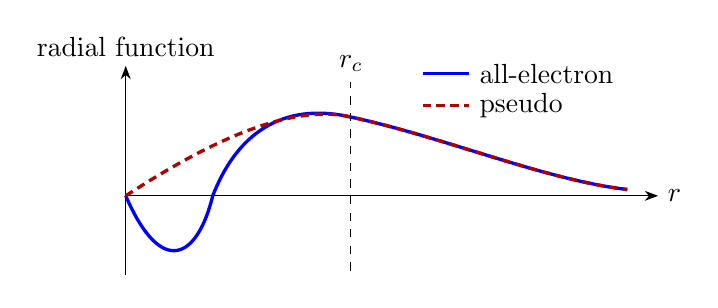
\begin{tikzpicture}[x=1.3cm,y=1cm,>=Stealth]
\draw[->] (0,0)--(5.2,0) node[right] {$r$};
\draw[->] (0,-1.0)--(0,1.65) node[above] {radial function};
\draw[dashed] (2.2,-0.95)--(2.2,1.45) node[above] {$r_c$};
\draw[very thick,blue] (0,0) .. controls (0.35,-1.05) and (0.7,-0.8) .. (0.85,0)
.. controls (1.15,1.0) and (1.7,1.15) .. (2.2,1.0)
.. controls (3.1,0.75) and (4.1,0.2) .. (4.9,0.08);
\draw[very thick,red!70!black,densely dashed] (0,0) .. controls (0.65,0.55) and (1.55,1.2) .. (2.2,1.0)
.. controls (3.1,0.75) and (4.1,0.2) .. (4.9,0.08);
\draw[blue,very thick] (2.9,1.55)--(3.35,1.55) node[right,black] {all-electron};
\draw[red!70!black,very thick,densely dashed] (2.9,1.15)--(3.35,1.15) node[right,black] {pseudo};
\end{tikzpicture}

\small Schematic only: smooth replacement inside $r_c$, matching outside. The number of depicted inner nodes is illustrative, not a computed Na $3s$ radial solution.
\end{center}

\section*{Primary references used for checks}
\begin{itemize}
\item \href{https://journals.aps.org/pr/abstract/10.1103/PhysRev.136.B864}{P. Hohenberg and W. Kohn, Phys. Rev. 136, B864 (1964)} and
\href{https://journals.aps.org/pr/abstract/10.1103/PhysRev.140.A1133}{W. Kohn and L. J. Sham, Phys. Rev. 140, A1133 (1965)}: the density-functional and auxiliary-orbital framework.
\item \href{https://journals.aps.org/pr/abstract/10.1103/PhysRev.116.287}{J. C. Phillips and L. Kleinman, ``New Method for Calculating Wave Functions in Crystals and Molecules,'' Phys. Rev. 116, 287 (1959)}: OPW orthogonality and the effective repulsive potential.
\item \href{https://physics.nist.gov/cgi-bin/Elements/elInfo.pl?context=text\&element=11}{NIST elemental data for sodium}.
The ground configuration is $[\mathrm{Ne}]3s$. The first ionization energy is $5.13907696\,\mathrm{eV}$.
\end{itemize}

\chapter{Solid State Theory: April 26, 2017 --- Solutions}
\label{s:theory-2017-04-midterm}
\begin{sourceNote}
These solutions are independently derived, not an official answer key. Reciprocal vectors satisfy $\mathbf g_i\cdot\mathbf t_j=2\pi\delta_{ij}$. Unless otherwise stated, a density of states is per unit area, per spin, and for the specified band or patch.
\end{sourceNote}

\section*{1. Translation symmetry and the first Brillouin zone}
\textbf{(a) False.} Atomic positions in a crystal have the general form
\[
\mathbf r_{\ell\alpha}=\mathbf R_\ell+\mathbf d_\alpha,\qquad
\mathbf R_\ell=\sum_i n_i\mathbf t_i.
\]
Atoms occupying the same basis site $\alpha$ in different cells are related by a Bravais translation. However, atoms of the same chemical species can occupy different basis sites. Diamond provides a counterexample: an FCC Bravais lattice with basis $\mathbf d_1=0$ and $\mathbf d_2=(a/4)(1,1,1)$. Both sites are carbon, but their separation is not an FCC translation. Chemical identity does not imply translational equivalence.

\textbf{(b) True.} The first Brillouin zone is the reciprocal-space Wigner-Seitz cell about the origin:
\[
\mathcal B_1=\{\mathbf k:\ |\mathbf k|\leq |\mathbf k-\mathbf G|
\text{ for every reciprocal vector }\mathbf G\}.
\]
A point outside this closed region violates at least one inequality. Thus some $\mathbf G\neq0$ satisfies $|\mathbf k-\mathbf G|<|\mathbf k|$. Boundary points can be equidistant from two reciprocal sites; they are not strictly outside the closed first zone.

\section*{2. FCC plane spacing and planar density}
The primitive volume and reciprocal vectors are
\[
\Omega=\mathbf t_1\cdot(\mathbf t_2\times\mathbf t_3)=\frac{a^3}{4},
\]
\[
\mathbf g_1=\frac{2\pi}{a}(-1,1,1),\quad
\mathbf g_2=\frac{2\pi}{a}(1,-1,1),\quad
\mathbf g_3=\frac{2\pi}{a}(1,1,-1).
\]
Their dot products verify $\mathbf g_i\cdot\mathbf t_j=2\pi\delta_{ij}$. If $\mathbf G=\sum_i m_i\mathbf g_i$ with relatively prime integer coefficients, then
\[
\mathbf G\cdot\mathbf R=2\pi\sum_i m_i n_i=2\pi\ell,\qquad \ell\in\mathbb Z.
\]
Because $\gcd(m_1,m_2,m_3)=1$, every integer $\ell$ occurs. Successive planes containing lattice points therefore have spacing $2\pi/|\mathbf G|$. A merely parallel vector cannot be substituted without checking its length and integer coefficients.

\subsection*{(a) A normal with half-integer reciprocal coefficients}
The shortest nonzero reciprocal vector parallel to $\mathbf g_1/2+\mathbf g_2-\mathbf g_3$ is
\[
\mathbf G=\mathbf g_1+2\mathbf g_2-2\mathbf g_3
=\frac{2\pi}{a}(-1,-3,5).
\]
The coefficients $(1,2,-2)$ are relatively prime, giving
\[
\boxed{d=\frac{2\pi}{|\mathbf G|}=\frac{a}{\sqrt{35}}.}
\]

\subsection*{(b) Number of lattice points per unit plane area}
On the plane through the origin, $n_1+2n_2-2n_3=0$. Every in-plane lattice vector is uniquely
\[
\mathbf R=n_2\underbrace{(-2\mathbf t_1+\mathbf t_2)}_{\mathbf u}
+n_3\underbrace{(2\mathbf t_1+\mathbf t_3)}_{\mathbf v}.
\]
This proves that $\mathbf u,\mathbf v$ form a primitive planar basis, not a supercell. In Cartesian coordinates,
\[
\mathbf u=\frac a2(1,-2,-1),\quad
\mathbf v=\frac a2(1,3,2),\quad
\mathbf u\times\mathbf v=\frac{a^2}{4}(-1,-3,5).
\]
The planar cell has area $A_\parallel=a^2\sqrt{35}/4$ and contains one lattice point. Therefore
\[
\boxed{\sigma=\frac{1}{A_\parallel}=\frac{4}{a^2\sqrt{35}}.}
\]
As a check, $A_\parallel d=\Omega$, so $\sigma=d/\Omega$. This counts Bravais lattice points. Multiplying again by the four points in an FCC conventional cell would count the cell conversion twice.

\subsection*{(c) A normal in the direct-lattice basis}
First convert the specified normal to Cartesian coordinates:
\[
\mathbf N=\mathbf t_1+2\mathbf t_2-2\mathbf t_3=\frac a2(0,-1,3).
\]
For a reciprocal vector $\mathbf G'\parallel\mathbf N$, the integer coefficients have ratio
\[
m_1:m_2:m_3=(\mathbf N\cdot\mathbf t_1):
(\mathbf N\cdot\mathbf t_2):(\mathbf N\cdot\mathbf t_3)=2:3:-1.
\]
The shortest such reciprocal vector is
\[
\mathbf G'=2\mathbf g_1+3\mathbf g_2-\mathbf g_3
=\frac{2\pi}{a}(0,-2,6),\qquad
\boxed{d'=\frac{a}{2\sqrt{10}}.}
\]
Independently, the projection of
$\mathbf R=(a/2)(n_2+n_3,n_1+n_3,n_1+n_2)$
onto $(0,-1,3)/\sqrt{10}$ is
$a(2n_1+3n_2-n_3)/(2\sqrt{10})$.
The numerator takes every integer value. The vector $(2\pi/a)(0,-1,3)$ is not an FCC reciprocal lattice vector; using it would miss the factor of two.

\section*{3. Critical points and local density of states}
The stated two-dimensional graphite model describes the two $\pi$ bands of a honeycomb layer. Set
\[
x=ak_x,\quad y=ak_y,\quad
h(x,y)=|F_{\mathbf k}|^2
=1+4\cos(x/2)\cos(\sqrt3y/2)+4\cos^2(x/2).
\]
Where $h>0$, $\nabla\epsilon_\pm=\pm\gamma\nabla h/(2\sqrt h)$. At $h=0$, this formula cannot be evaluated by interpreting $0/0$ as zero.

\subsection*{(a) Expansions at the three points}
\textbf{$\Gamma$: smooth extrema.} With $\mathbf q=\mathbf k$,
\[
h=9-\frac32a^2(q_x^2+q_y^2)+O(a^4q^4),\qquad
|F|=3-\frac14a^2q^2+O(a^4q^4).
\]
Thus, with $\alpha=\gamma a^2/4>0$,
\[
\epsilon_+=\epsilon_p+3\gamma-\alpha q^2+O(q^4),\qquad
\epsilon_-=\epsilon_p-3\gamma+\alpha q^2+O(q^4).
\]
Both gradients vanish. The upper band has a local maximum, a negative-definite Hessian, and Morse index 2; the lower band has a local minimum, a positive-definite Hessian, and index 0.

\textbf{$Q$: a saddle in each band.} At $(x,y)=(\pi,\pi/\sqrt3)$,
\[
h=1,\quad \nabla h=0,\quad
H_h=\begin{pmatrix}2&\sqrt3\\ \sqrt3&0\end{pmatrix}.
\]
Its eigenvalues are $3,-1$, with orthonormal directions
$\hat{\mathbf u}=(\sqrt3/2,1/2)$ and $\hat{\mathbf v}=(-1/2,\sqrt3/2)$.
For displacement components $q_u,q_v$,
\[
\epsilon_\pm=\epsilon_p\pm\gamma
\pm\frac{\gamma a^2}{4}(3q_u^2-q_v^2)+O(a^3q^3).
\]
The curvatures have opposite signs, so both bands have saddles of index 1. Being on a zone boundary does not invalidate this local classification: the dispersion extends periodically.

\textbf{$P$: a Dirac contact, not an ordinary smooth stationary point.}
At $(x,y)=(4\pi/3,0)$, $h=0$, while
\[
h=\frac34a^2q^2+O(a^3q^3),\qquad
\epsilon_\pm=\epsilon_p\pm c|\mathbf q|+O(q^2),\qquad
c=\frac{\sqrt3\gamma a}{2}.
\]
The upper band has a conical local minimum and the lower band a conical local maximum, and the bands touch. Each energy-ordered band is nondifferentiable at the cone tip. Its gradient does not exist; it is not a smooth van Hove or Morse stationary point satisfying $\nabla\epsilon=0$. If the term critical point includes band-degeneracy singularities, identify $P$ explicitly as a \emph{Dirac band-contact singularity}. The directional slopes are finite, not infinite. A quadratic-extremum DOS formula is inapplicable.

\begin{center}
\begin{minipage}{0.95\linewidth}
\centering
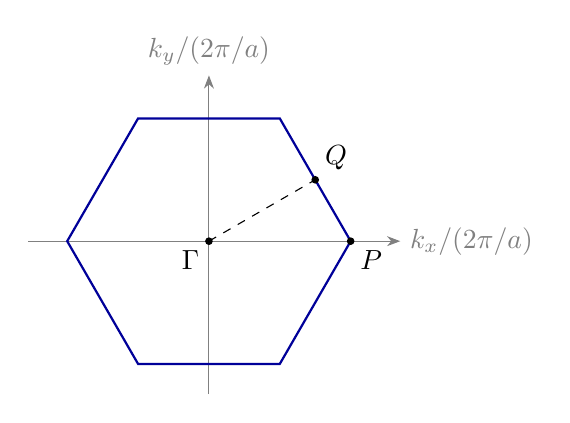
\begin{tikzpicture}[scale=2.7,>=Stealth]
\draw[->,gray] (-.85,0)--(.9,0) node[right] {$k_x/(2\pi/a)$};
\draw[->,gray] (0,-.72)--(0,.78) node[above] {$k_y/(2\pi/a)$};
\draw[thick,blue!60!black] (2/3,0)--(1/3,.57735)--(-1/3,.57735)--(-2/3,0)--(-1/3,-.57735)--(1/3,-.57735)--cycle;
\fill (0,0) circle(.018) node[below left] {$\Gamma$};
\fill (.5,.288675) circle(.018) node[above right] {$Q$};
\fill (2/3,0) circle(.018) node[below right] {$P$};
\draw[dashed] (0,0)--(.5,.288675);
\end{tikzpicture}
\par\small
The reconstructed first Brillouin zone places $Q$ at an edge midpoint and $P$ at a corner, using the question's coordinates.
\end{minipage}
\end{center}

\subsection*{(b) Choosing $\Gamma$: direct evaluation of the local DOS}
Choose a disk $q<\Lambda\ll a^{-1}$ and let $E_{\min}=\epsilon_p-3\gamma$. The number of states per unit sample area per $k$-space area is $(2\pi)^{-2}$. In the quadratic approximation,
\begin{align*}
g_{\Gamma,-}(E)
&=\frac1{(2\pi)^2}\int_{q<\Lambda}\dd^2q\,
\delta(E-E_{\min}-\alpha q^2)\\
&=\frac1{2\pi}\int_0^\Lambda q\,\dd q\,
\delta(E-E_{\min}-\alpha q^2)\\
&=\boxed{\frac1{\pi\gamma a^2}
\Theta(E-E_{\min})\Theta(E_{\min}+\alpha\Lambda^2-E).}
\end{align*}
This is the step onset of a two-dimensional quadratic minimum. For the upper band,
\[
g_{\Gamma,+}(E)=\frac1{\pi\gamma a^2}
\Theta(E_{\max}-E)\Theta(E-E_{\max}+\alpha\Lambda^2),
\quad E_{\max}=\epsilon_p+3\gamma.
\]
These are approximate contributions from the chosen patch, not the complete band DOS. Multiply by $A_c=\sqrt3a^2/2$ for DOS per primitive cell, by 2 for both spins, or by sample area $A$ for total DOS. Integrating either expression over energy gives $\Lambda^2/(4\pi)$, the number of states in the chosen disk per unit sample area.

For comparison, one $Q$ saddle produces a logarithmic singularity. One $P$ valley, with its upper and lower conical branches, gives
\[
g_P(E)=\frac{|E-\epsilon_p|}{2\pi c^2}
=\frac{2|E-\epsilon_p|}{3\pi\gamma^2a^2}.
\]
Spin and the second inequivalent valley have not been included. The DOS vanishes at the Dirac point; it is not the constant DOS of a two-dimensional parabolic band edge.

\section*{4. Bloch's theorem}
For a one-electron Hamiltonian with $V(\mathbf r+\mathbf R)=V(\mathbf r)$, energy eigenstates can be chosen as
\[
\boxed{\psi_{n\mathbf k}(\mathbf r)=\ee^{\ii\mathbf k\cdot\mathbf r}
u_{n\mathbf k}(\mathbf r),\qquad
u_{n\mathbf k}(\mathbf r+\mathbf R)=u_{n\mathbf k}(\mathbf r).}
\]
Equivalently, $\psi_{n\mathbf k}(\mathbf r+\mathbf R)=
\ee^{\ii\mathbf k\cdot\mathbf R}\psi_{n\mathbf k}(\mathbf r)$.
The Hamiltonian commutes with all lattice translations, which also commute with one another. Simultaneous eigenstates may be chosen; the translation-group multiplication law fixes their translation eigenvalues to the displayed phase form. Here $n$ is a band index, and $\mathbf k,\mathbf k+\mathbf G$ are equivalent quasimomentum labels. The Bloch wave itself need not be periodic; its probability density and its periodic factor $u_{n\mathbf k}$ are periodic.

\section*{5. Why exchange lowers the interaction energy}
Let $x=(\mathbf r,\sigma)$ include spin and let $w(\mathbf r-\mathbf r')=e^2/(4\pi\varepsilon_0|\mathbf r-\mathbf r'|)$. For a fixed orthonormal set of spin-orbitals,
\begin{align*}
J_{ij}&=\int\dd x\,\dd x'\,|\chi_i(x)|^2w(\mathbf r-\mathbf r')|\chi_j(x')|^2,\\
K_{ij}&=\int\dd x\,\dd x'\,\chi_i^*(x)\chi_j(x)
w(\mathbf r-\mathbf r')\chi_j^*(x')\chi_i(x').
\end{align*}
A Hartree product lacks exchange cross terms. Antisymmetrizing into a Slater determinant gives
\[
E^{\rm HF}_{ee}=\frac12\sum_{ij}(J_{ij}-K_{ij}).
\]
Since $J_{ii}=K_{ii}$, self-interaction cancels. Relative to the same-orbital Hartree-product interaction energy $E^{\rm H}_{ee}=\tfrac12\sum_{i\ne j}J_{ij}$,
\[
E^{\rm HF}_{ee}-E^{\rm H}_{ee}=-\frac12\sum_{i\ne j}K_{ij}\leq0.
\]
The Coulomb kernel is positive definite, so $K_{ij}\geq0$; exchange between opposite-spin functions vanishes. If the reference is instead the full-density classical Hartree energy $\tfrac12\sum_{ij}J_{ij}$, the usual exchange functional is $E_x=-\tfrac12\sum_{ij}K_{ij}$, including the diagonal self-interaction correction.

Antisymmetry reduces the likelihood of same-spin electrons being close. This exchange hole reduces repulsion; no extra attractive force is introduced. The comparison fixes the orbitals and the Hartree reference. It does not prove universal strict ordering of separately optimized energies in every Hartree and HF variational convention.

\section*{6. The Hohenberg-Kohn functional}
Write $\hat H_v=\hat T+\hat W_{ee}+\sum_i v(\mathbf r_i)$. Under the usual nondegenerate-ground-state assumptions, the ground-state density determines the external potential up to a constant, and hence ground-state properties. A constrained-search expression for the universal functional is
\[
\boxed{F[n]=\min_{\Psi\to n}\langle\Psi|\hat T+\hat W_{ee}|\Psi\rangle.}
\]
The search is over normalized antisymmetric $N$-electron wavefunctions with density $n$. It contains kinetic and electron-electron energies but no explicit external potential. The latter enters separately:
\[
E_v[n]=F[n]+\int v(\mathbf r)n(\mathbf r)\,\dd^3r,\qquad
E_0=\min_{\substack{n\ {\rm admissible}\\ \int n=N}}E_v[n].
\]
The minimum occurs at the physical ground-state density. Where the functional derivative exists, the Euler equation is
$\delta F/\delta n(\mathbf r)+v(\mathbf r)=\mu$,
with $\mu$ enforcing electron number.
Universality does not imply that different potentials have the same minimizing density: changing $\int vn$ changes the minimum. Existence of the exact functional does not provide a practical explicit formula for it.

\section*{7. The local density approximation}
The Kohn-Sham decomposition is
\[
F[n]=T_s[n]+E_H[n]+E_{xc}[n],\qquad
E_H[n]=\frac12\int\dd^3r\dd^3r'\,n(\mathbf r)w(\mathbf r-\mathbf r')n(\mathbf r').
\]
$T_s$ is the kinetic energy of the auxiliary noninteracting system with the same density. $E_{xc}$ includes the interaction correction beyond classical Hartree energy and the difference between interacting kinetic energy and $T_s$. LDA uses the uniform-gas exchange-correlation energy \emph{per electron} at the local density:
\[
\boxed{E_{xc}^{\rm LDA}[n]=\int n(\mathbf r)
\varepsilon_{xc}^{\rm unif}(n(\mathbf r))\,\dd^3r.}
\]
The factor $n$ is required because $\varepsilon_{xc}^{\rm unif}$ is per electron. Its derivative gives
\[
v_{xc}^{\rm LDA}(\mathbf r)=
\left[\varepsilon_{xc}^{\rm unif}(n)+n\frac{\dd\varepsilon_{xc}^{\rm unif}}{\dd n}\right]_{n=n(\mathbf r)}.
\]
LDA treats an inhomogeneous system as locally uniform. It is motivated for slowly varying densities, omits explicit gradients and general nonlocal information, and is not exact for arbitrary systems. Dependence on $n_\uparrow,n_\downarrow$ gives the local spin-density approximation.

\section*{8. Hartree, Hartree-Fock, and Kohn-Sham equations}
The common one-body operator is
\[
\hat h_0=-\frac{\hbar^2}{2m}\nabla^2+v_{\rm ext}(\mathbf r).
\]
The terms are electron kinetic energy and the external potential from fixed nuclei and other external sources. Periodic calculations use Bloch orbitals and sums over occupied $\mathbf k$ points.

\subsection*{Hartree: the product-state mean field}
\[
\boxed{\left[\hat h_0+\sum_{j\ne i}J_j(\mathbf r)\right]\chi_i(x)
=\varepsilon_i\chi_i(x),\quad
J_j(\mathbf r)=\int\dd x'\,w(\mathbf r-\mathbf r')|\chi_j(x')|^2.}
\]
Each electron experiences the other electrons' average Coulomb potential. The restriction $j\ne i$ excludes its own orbital's self-interaction. The approximation omits exchange from antisymmetry and genuine many-electron correlation.

\subsection*{Hartree-Fock: a single Slater determinant}
\[
\boxed{\left[\hat h_0+\sum_j(\hat J_j-\hat K_j)\right]\chi_i
=\varepsilon_i\chi_i,}
\]
where $\hat J_j\chi_i=J_j(\mathbf r)\chi_i(x)$ and
\[
(\hat K_j\chi_i)(x)=\chi_j(x)\int\dd x'\,
w(\mathbf r-\mathbf r')\chi_j^*(x')\chi_i(x').
\]
The exchange operator is nonlocal: its value at $x$ depends on orbital values elsewhere. For $j=i$, exchange cancels the direct term. HF optimizes single determinants, not the full interacting many-electron Hilbert space.

\subsection*{Kohn-Sham: an auxiliary system reproducing the density}
\[
\boxed{\left[-\frac{\hbar^2}{2m}\nabla^2+v_{\rm ext}(\mathbf r)
+v_H(\mathbf r)+v_{xc}(\mathbf r)\right]\phi_i
=\epsilon_i\phi_i,}
\]
\[
v_H(\mathbf r)=\int\dd^3r'\,w(\mathbf r-\mathbf r')n(\mathbf r'),\quad
v_{xc}(\mathbf r)=\frac{\delta E_{xc}}{\delta n(\mathbf r)},\quad
n(\mathbf r)=\sum_i f_i|\phi_i(\mathbf r)|^2.
\]
Use spin-orbitals with $f_i\leq1$, or unpolarized spatial orbitals with $f_i\leq2$, without counting spin twice. The orbital kinetic energy $T_s$ generally differs from the interacting kinetic energy; the difference is included in $E_{xc}$.
The electronic total energy is
\begin{align*}
E&=T_s+\int v_{\rm ext}n\,\dd^3r+E_H+E_{xc}\\
 &=\sum_i f_i\epsilon_i-E_H+E_{xc}-\int n v_{xc}\,\dd^3r.
\end{align*}
Summing orbital eigenvalues alone double-counts mean-field contributions. Add fixed nuclear repulsion $E_{NN}$ if the total electron-plus-nuclei energy is required.

\subsection*{Self-consistent solution}
All three problems are nonlinear because their effective operators depend on the unknown orbitals or density. Choose a basis or grid and boundary conditions; guess orbitals or a density; build the direct, exchange, or exchange-correlation terms; solve the eigenvalue problem; occupy states for the required electron number; compute and usually mix the new density; rebuild and repeat. Check density, total-energy, and equation-residual convergence, followed by basis, grid, and $\mathbf k$-mesh convergence. Different initial densities or spin states can reach different stationary solutions. SCF convergence alone does not establish a global minimum.

\section*{Primary references and verification scope}
The graphite model is discussed in
\href{https://doi.org/10.1103/PhysRev.71.622}{P. R. Wallace, The Band Theory of Graphite (1947)}.
The expansions, lattice-plane calculations, and DOS normalization above follow directly from the question data.
Density-functional foundations are given in
\href{https://doi.org/10.1103/PhysRev.136.B864}{Hohenberg and Kohn, Inhomogeneous Electron Gas (1964)}
and
\href{https://doi.org/10.1103/PhysRev.140.A1133}{Kohn and Sham, Self-Consistent Equations Including Exchange and Correlation Effects (1965)}.

\chapter{Solutions: Midterm Exam, November 8, 2017}
\label{s:physics-2017-11-midterm}
The density of states $D(E)$ below counts states per unit energy in the entire sample of volume $V$. A factor $g_s$ explicitly specifies spin counting. We use $g_s=2$ for the unpolarized free-electron gas.

\section*{1. A change of primitive basis}
Let $T=(\vct t_1\ \vct t_2\ \vct t_3)$ and $S=(\vct s_1\ \vct s_2\ \vct s_3)$. The stated relations give $S=TA$, where
\[
A=\begin{pmatrix}2&-1&1\\-1&1&\alpha\\2&\alpha&1\end{pmatrix},
\qquad
\det A=-(2\alpha+1)(\alpha+1)=-2\alpha^2-3\alpha-1.
\]
Two primitive bases generate the same lattice precisely when their change-of-basis matrix is \emph{integer unimodular}: $A$ has integer entries and $\det A=\pm1$. Necessity follows because both sets of basis vectors must be integer combinations of the other set. Sufficiency follows from the adjugate formula: an integer matrix with determinant $\pm1$ has an integer inverse.

The determinant equation $\det A=+1$ gives $2\alpha^2+3\alpha+2=0$, whose discriminant is $-7$. The equation $\det A=-1$ gives
\[
\alpha(2\alpha+3)=0,
\qquad \alpha=0\ \text{or}\ -\frac32.
\]
The second root gives noninteger coordinates for $\vct s_2$ and $\vct s_3$ in the original primitive basis; equal cell volumes alone do not make it a basis of the same lattice. Therefore
\[
\boxed{\alpha=0}.
\]
As a direct sufficiency check, at $\alpha=0$ the inverse relations are
\[
\vct t_1=-\vct s_1-\vct s_2+2\vct s_3,\qquad
\vct t_2=-\vct s_1+2\vct s_3,\qquad
\vct t_3=\vct s_1+\vct s_2-\vct s_3.
\]
They express every original lattice point as an integer combination of the new primitive vectors.

\section*{2. Silicon as a lattice and a basis}
Crystalline silicon has the diamond structure: an fcc Bravais lattice with two identical Si atoms in each primitive cell. Using the conventional cubic lattice constant $a$, one may choose
\[
\vct t_1=\frac a2(0,1,1),\quad
\vct t_2=\frac a2(1,0,1),\quad
\vct t_3=\frac a2(1,1,0),
\qquad
\vct\tau_1=(0,0,0),\quad
\vct\tau_2=\frac a4(1,1,1).
\]
The full set of atomic positions is $\vct R+\vct\tau_\nu$, with $\vct R$ an integer combination of the three translations. The conventional cubic cell contains four fcc lattice points and hence eight Si atoms; the primitive cell contains two.

\section*{3. The stated bcc lattice with a two-atom basis}
\begin{sourceNote}
The source explicitly specifies \emph{two atoms per primitive cell}. This is followed below. It is different from a monatomic bcc crystal, which has one atom per primitive cell and two per conventional cubic cell. The unspecified two-atom basis changes the atomic count, but not the Bravais-cell or Brillouin-zone volumes under the stated bcc assumption.
\end{sourceNote}
\subsection*{(a) Atomic number density}
A conventional bcc cube contains $8(1/8)+1=2$ lattice points. Its primitive volume is thus $\Omega=a^3/2$. With two atoms per primitive cell,
\[
\boxed{n_{\rm atom}=\frac2\Omega=\frac4{a^3}}.
\]
If the intended premise had instead been monatomic bcc, the density would be $2/a^3$; that is not the literal premise of this question.

\subsection*{(b) Wigner--Seitz-cell volume}
A Wigner--Seitz cell contains one Bravais lattice point and has the primitive volume:
\[
\boxed{V_{\rm WS}=\frac{a^3}{2}}.
\]

\subsection*{(c) Brillouin-zone volume}
The Brillouin zone is a reciprocal Wigner--Seitz cell, so
\[
\boxed{V_{\rm BZ}=\frac{(2\pi)^3}{\Omega}=\frac{16\pi^3}{a^3}}.
\]

\subsection*{(d) Number of facets}
The reciprocal lattice of bcc is fcc. In units $2\pi/a$, its shortest nonzero reciprocal vectors are
\[
(\pm1,\pm1,0),\quad(\pm1,0,\pm1),\quad(0,\pm1,\pm1).
\]
There are twelve. Each perpendicular-bisector plane
$\vct k\cdot\vct G=|\vct G|^2/2$ supplies one face of the reciprocal Wigner--Seitz cell. The resulting polyhedron is a rhombic dodecahedron with
\[
\boxed{12\ \text{facets}}.
\]
The fourteen-faced truncated octahedron is the \emph{direct-space} Wigner--Seitz cell of bcc, not its first Brillouin zone.

\section*{4. Reciprocal vectors and planar density}
\subsection*{(a) Reciprocal primitive vectors}
The direct primitive volume is $\Omega=a^3/4$. The cross-product formula gives
\[
\vct g_1=\frac{2\pi}{\Omega}(\vct t_2\times\vct t_3),
\]
with cyclic permutations for the other two vectors. Therefore
\[
\boxed{\vct g_1=\frac{2\pi}{a}(-1,1,1),\quad
\vct g_2=\frac{2\pi}{a}(1,-1,1),\quad
\vct g_3=\frac{2\pi}{a}(1,1,-1)}.
\]
For instance, the first direct vector has dot product $2\pi$ with $\vct g_1$ and zero with $\vct g_2,\vct g_3$, verifying the required normalization.

\subsection*{(b) Density on successive lattice planes}
Let $A_{\parallel}$ be the primitive area of the two-dimensional lattice on one plane, containing one lattice point. Successive occupied planes are separated by $d$. The primitive prism obtained from two in-plane translations and one translation to the next plane has volume $A_{\parallel}d=\Omega$; a lateral shift of the next layer does not affect this volume. Thus
\[
\boxed{\sigma=\frac1{A_{\parallel}}=\frac d\Omega=\frac{4d}{a^3}}.
\]
A second derivation counts points in a large slab: $L/d$ layers of area $A$ contain approximately $\sigma A L/d$ points, which must equal $AL/\Omega$. Boundary corrections vanish in the macroscopic limit.

\section*{5. The Born--von Karman sum}
Define
\[
F(\vct k)=k_xk_yk_z\exp(-k_x^2/\alpha-k_y^2/\beta-k_z^2/\gamma).
\]
The allowed wave vectors of a Born--von Karman periodic box form an inversion-symmetric set: if $\vct k$ is allowed, so is $-\vct k$. Since the Gaussian is even and the product of three components is odd,
\[
F(-\vct k)=-F(\vct k).
\]
Every pair cancels, and the unpaired origin contributes zero. The positive parameters ensure absolute convergence, so pairing the infinite sum is legitimate. Consequently
\[
\boxed{\frac1V\sum_{\vct k}F(\vct k)=0}.
\]
This is an exact discrete cancellation, not merely a continuum approximation. In the thermodynamic limit it also follows by replacing $V^{-1}\sum_{\vct k}$ by $(2\pi)^{-3}\int\dd^3k$; each Cartesian odd Gaussian integral vanishes.

\section*{6. Translating a wavefunction between cells}
Put $\vct T=\vct t_m-\vct t_n$. A point $\vct r$ in the cell centered on $\vct t_m$ corresponds to $\vct r-\vct T$ in the cell centered on $\vct t_n$. Bloch's theorem says
\[
\psi_{\vct k}(\vct r)=\ee^{\ii\vct k\cdot\vct T}
\psi_{\vct k}(\vct r-\vct T).
\]
Since the latter function is known as $f$ in the original cell,
\[
\boxed{\psi_{\vct k}(\vct r)
=\ee^{\ii\vct k\cdot(\vct t_m-\vct t_n)}
f\bigl(\vct r-(\vct t_m-\vct t_n)\bigr)}.
\]
Equivalently, with the same local coordinate $\vct\rho$ in both cells,
$\psi(\vct t_m+\vct\rho)=\ee^{\ii\vct k\cdot\vct T}f(\vct t_n+\vct\rho)$.
Both the phase and the shifted function argument are required when $f$ is expressed in the original global coordinate system.

\section*{7. The anisotropic parabolic band}
\subsection*{(a) Critical point and its type}
The gradient and Hessian are
\[
\nabla_{\vct k}\varepsilon=
\left(\frac{2(k_x-k_0)}\alpha,\frac{2k_y}\beta,\frac{2k_z}\gamma\right),
\qquad H=\operatorname{diag}(2/\alpha,2/\beta,2/\gamma).
\]
All three Hessian eigenvalues are positive. Hence
\[
\boxed{\vct k_c=(k_0,0,0),\qquad \varepsilon_c=\varepsilon_0,
\qquad \text{type }M_0\ \text{(minimum)}}.
\]

\subsection*{(b) Density of states}
For $\Delta=E-\varepsilon_0\ge0$, the states below $E$ occupy an ellipsoid with semiaxes
$\sqrt{\alpha\Delta}$, $\sqrt{\beta\Delta}$, and $\sqrt{\gamma\Delta}$. Its volume is
$(4\pi/3)\sqrt{\alpha\beta\gamma}\,\Delta^{3/2}$. There is one allowed wave vector per volume $(2\pi)^3/V$ in reciprocal space. Thus the integrated state count is
\[
\mathcal N(E)=\frac{g_sV\sqrt{\alpha\beta\gamma}}{6\pi^2}
(E-\varepsilon_0)^{3/2}\Theta(E-\varepsilon_0).
\]
Differentiation gives
\[
\boxed{D(E)=\frac{g_sV\sqrt{\alpha\beta\gamma}}{4\pi^2}
\sqrt{E-\varepsilon_0}\,\Theta(E-\varepsilon_0)}.
\]
Use $g_s=1$ for a spin-resolved band, or $g_s=2$ for a band whose two spin states are counted together. Translation of the ellipsoid by $k_0$ leaves its volume unchanged. If the parabola is only a local band-edge approximation, this expression applies near that edge, before other band features or zone boundaries matter.

\section*{8. Three valence electrons per atom in an fcc metal}
An fcc conventional cell contains four atoms. The stated three valence electrons per atom therefore give
\[
n=\frac NV=\frac{12}{a^3}.
\]
By definition, $4\pi(r_sa_0)^3/3=1/n$, where $a_0$ is the Bohr radius. Hence
\[
\boxed{r_s=\frac{a}{(16\pi)^{1/3}a_0}}.
\]
Counting the two spin states in a filled Fermi sphere gives
$n=k_F^3/(3\pi^2)$, so
\[
\boxed{k_F=\frac{(36\pi^2)^{1/3}}a},\qquad
\boxed{\varepsilon_F=\frac{\hbar^2}{2m_ea^2}(36\pi^2)^{2/3}}.
\]
Finally,
\[
\overline\varepsilon
=\frac{\int_0^{k_F}(\hbar^2k^2/2m_e)k^2\dd k}
{\int_0^{k_F}k^2\dd k}
=\frac{\hbar^2}{2m_e}\frac{k_F^5/5}{k_F^3/3}
=\boxed{\frac35\varepsilon_F}.
\]
This uses the stipulated free-electron model; it does not assume that actual multivalent-metal bands are exactly free-electron dispersions.

\section*{9. Sommerfeld expansion at fixed particle number}
The expansion requires $T\ll T_F$ and a density of states smooth near the chemical potential. The density of states is zero below the bottom of the band, so the printed lower integration limit $-\infty$ is harmless.

\subsection*{(a) Temperature derivative of the chemical potential}
Apply the supplied formula with $\Gamma=D$:
\[
N=\int_{-\infty}^{\mu(T)}D(E)\dd E
+\frac{\pi^2}{6}\kb^2T^2D'(\mu(T))+O(T^4).
\]
At fixed $N$ and volume, differentiation gives
\[
0=D(\mu)\mu'
+\frac{\pi^2}{3}\kb^2T D'(\mu)
+\frac{\pi^2}{6}\kb^2T^2D''(\mu)\mu'+O(T^3),
\]
where $\mu'=\dd\mu/\dd T$. The leading change in $\mu$ is quadratic in $T$, so $\mu'=O(T)$ and the third term is $O(T^3)$. Keeping the requested order,
\[
\boxed{\frac{\dd\mu}{\dd T}
=-\frac{\pi^2}{3}\kb^2T\frac{D'(\mu)}{D(\mu)}+O(T^3)}.
\]
The volume is fixed, so no temperature-dependent volume factor is differentiated.

\subsection*{(b) The three-dimensional free-electron result}
For $E>0$, $D(E)=C\sqrt E$ and $D'/D=1/(2E)$. Therefore
\[
\frac{\dd\mu}{\dd T}=-\frac{\pi^2\kb^2T}{6\mu}+O(T^3).
\]
Multiply by $2\mu$ and integrate from $0$ to $T$:
\[
\mu(T)^2=\mu_0^2-\frac{\pi^2}{6}\kb^2T^2+O(T^4).
\]
Expanding the positive square root, and using $\mu_0=\varepsilon_F=\kb T_F$, yields
\[
\boxed{\mu(T)=\mu_0\left[1-\frac{\pi^2}{12}
\left(\frac T{T_F}\right)^2\right]+O(T^4)}.
\]
Here and below, the remainder notation in dimensional formulas carries the appropriate constant energy and temperature scales.

\subsection*{(c) Internal energy}
Set $\Gamma(E)=E D(E)$. Then $\Gamma'(E)=D(E)+E D'(E)$, giving
\[
\boxed{U(T)=\int_{-\infty}^{\mu(T)}E D(E)\dd E
+\frac{\pi^2}{6}(\kb T)^2
\bigl[D(\mu(T))+\mu(T)D'(\mu(T))\bigr]+O(T^4)}.
\]
The upper limit changes with temperature because the number of electrons is held fixed.

\subsection*{(d) Constant-volume electronic heat capacity}
Differentiate the preceding expression along the fixed-$N$ solution $\mu(T)$:
\begin{align*}
C_V&=\mu D(\mu)\mu'
+\frac{\pi^2}{3}\kb^2T\bigl[D(\mu)+\mu D'(\mu)\bigr]+O(T^3)\\
&=-\frac{\pi^2}{3}\kb^2T\mu D'(\mu)
+\frac{\pi^2}{3}\kb^2T\bigl[D(\mu)+\mu D'(\mu)\bigr]+O(T^3)\\
&=\frac{\pi^2}{3}\kb^2T D(\mu)+O(T^3).
\end{align*}
The two terms involving $\mu D'$ cancel. Since $\mu-\mu_0=O(T^2)$, replacing $D(\mu)$ by $D(\mu_0)$ changes only the cubic correction:
\[
\boxed{C_V(T)=\frac{\pi^2}{3}\kb^2T D(\mu_0)+O(T^3)}.
\]

\subsection*{(e) Why the classical value is strongly suppressed}
Deep occupied states cannot be thermally rearranged freely because of Pauli exclusion. Only a shell of width of order $\kb T$ near $\varepsilon_F$ contributes appreciably. In three dimensions,
\[
D(\varepsilon_F)=\frac{3N}{2\varepsilon_F},\qquad
N_{\rm active}\sim D(\varepsilon_F)\kb T=\frac32N\frac T{T_F}.
\]
Estimating an order-$\kb$ contribution per active state reproduces the printed scale
$C_V\sim(3/2)N\kb(T/T_F)$ and explains why it is much smaller than the classical $(3/2)N\kb$.

\textbf{The printed estimate does not have the exact coefficient.} Substitution of the same $D(\varepsilon_F)$ into part (d) instead gives
\[
\boxed{C_V=\frac{\pi^2}{2}N\kb\frac T{T_F}
+O\!\left(N\kb(T/T_F)^3\right)}.
\]
Thus part (e) is a qualitative active-electron argument. Treating its factor $3/2$ as exact would contradict part (d).

\section*{References and checks}
The lattice, state-counting, and Sommerfeld derivations are displayed explicitly above. For the statistical-mechanical assumptions and low-temperature expansion, see
\href{https://www.damtp.cam.ac.uk/user/tong/statphys/statmechhtml/S3.html}{David Tong, Statistical Physics, Chapter 3}.
The accompanying verification script independently counts finite lattice samples and integrates the finite-temperature Fermi distribution to check the limiting coefficients.

\chapter{Solid State Theory: Final, June 24, 2020}
\label{s:theory-2020-06-final}
\begin{sourceNote}
All twelve visible questions are addressed. The supplied page has a total weight of 85\%. The derivations below distinguish an exchange operator from an exchange-correlation energy functional, and count bands per primitive cell rather than per conventional cubic cell.
\end{sourceNote}

\section*{1. Hartree and Hartree--Fock}
Write $x=(\vct r,\sigma)$ for position and spin. A Hartree trial state is a product,
\[
\Psi_{\mathrm H}(x_1,\ldots,x_N)=\prod_{i=1}^N\psi_i(x_i).
\]
It describes each electron moving in an average electrostatic field. The product itself is not antisymmetric under exchange of two electrons and does not generate the Fock exchange term. Hartree--Fock (HF) instead uses a Slater determinant of orthonormal spin orbitals,
\[
\Psi_{\mathrm{HF}}=\frac{1}{\sqrt{N!}}\det[\psi_i(x_j)].
\]
The determinant changes sign upon exchange and therefore implements the Pauli principle. Let $\hat h=-\hbar^2\nabla^2/(2m)+v_{\mathrm{ext}}$ and define
\begin{align*}
J_{ij}&=\iint |\psi_i(x)|^2\frac{e^2}{|\vct r-\vct r'|}|\psi_j(x')|^2\dd x\dd x',\\
K_{ij}&=\iint\psi_i^*(x)\psi_j(x)\frac{e^2}{|\vct r-\vct r'|}\psi_j^*(x')\psi_i(x')\dd x\dd x'.
\end{align*}
Then
\[
E_{\mathrm{HF}}=\sum_i\bra{\psi_i}\hat h\ket{\psi_i}
 +\frac12\sum_{ij}(J_{ij}-K_{ij}).
\]
For pure spin states, exchange acts only between equal spins. The terms with $i=j$ cancel because $J_{ii}=K_{ii}$; an electron does not interact with itself in HF. The Hartree product energy contains the direct interactions with $j\ne i$ but no exchange. A common density-only Hartree approximation includes self-interaction unless it is separately removed.

HF treats exchange exactly within a single determinant. It still misses correlation beyond that determinant. Its exchange operator is generally nonlocal; it must not be identified with the local Kohn--Sham exchange-correlation potential.

\section*{2. Fully spin-polarized homogeneous gas}
Hold $N$ and $V$ fixed. In the normal, unpolarized state, two spin species occupy equal Fermi spheres, so
\[
n=\frac{2}{(2\pi)^3}\frac{4\pi k_F^3}{3}
 =\frac{k_F^3}{3\pi^2}.
\]
In the fully polarized state only one spin species is occupied:
\[
n=\frac{(k_F^{\mathrm{FP}})^3}{6\pi^2},\qquad
k_F^{\mathrm{FP}}=2^{1/3}k_F.
\]
The kinetic energy per electron of a filled three-dimensional sphere is $3\hbar^2k_F^2/(10m)$. The exchange energy per electron of one occupied spin species is $-3e^2k_F/(4\pi)$. The latter has the same form in the normal state because each spin species exchanges only with itself. Therefore
\[
\boxed{E_0^{(\mathrm{FP})}=N\left[
2^{2/3}\frac35\frac{\hbar^2k_F^2}{2m}
-2^{1/3}\frac{3e^2k_F}{4\pi}\right].}
\]
The $k_F$ in this box is the \emph{normal-state} Fermi wavevector in the question. Reusing it as the polarized wavevector without the factor $2^{1/3}$ would violate particle-number conservation.

As a check, define the polarization $\zeta=(N_\uparrow-N_\downarrow)/N$. Since $k_{F\sigma}=k_F(1\pm\zeta)^{1/3}$,
\begin{align*}
\frac{T(\zeta)}N&=\frac35E_F
\frac{(1+\zeta)^{5/3}+(1-\zeta)^{5/3}}2,\\
\frac{E_x(\zeta)}N&=-\frac{3e^2k_F}{4\pi}
\frac{(1+\zeta)^{4/3}+(1-\zeta)^{4/3}}2.
\end{align*}
Setting $\zeta=0$ and $1$ recovers both states. Polarization raises kinetic energy and makes exchange more negative. It does not automatically lower their sum; the competition depends on density.

\section*{3. Equations and self-consistent solution}
For individually normalized Hartree orbitals, variation of the product-state energy gives
\[
\left[\hat h+\sum_{j\ne i}J_j(\vct r)\right]\psi_i(x)=\epsilon_i\psi_i(x),\qquad
J_j(\vct r)=\int\frac{e^2|\psi_j(x')|^2}{|\vct r-\vct r'|}\dd x'.
\]
Here $\hat h$ contains the kinetic energy and the fixed external potential, while $J_j$ is the electrostatic repulsion from orbital $j$. The explicitly excluded $i$ term avoids self-interaction in this product-state variational equation.

For HF, impose $\braket{\psi_i}{\psi_j}=\delta_{ij}$ using a Hermitian matrix of Lagrange multipliers. Variation of
\[
E_{\mathrm{HF}}-\sum_{ij}\lambda_{ij}
(\braket{\psi_i}{\psi_j}-\delta_{ij})
\]
with respect to $\psi_i^*$ yields a coupled orbital equation. A unitary rotation among occupied orbitals diagonalizes $\lambda$, giving the canonical form
\[
\boxed{\left[\hat h+\sum_j(\hat J_j-\hat K_j)\right]\psi_i
=\epsilon_i\psi_i.}
\]
The exchange operator acts as
\[
(\hat K_j\psi_i)(x)=\psi_j(x)\int
\frac{e^2\psi_j^*(x')\psi_i(x')}{|\vct r-\vct r'|}\dd x'.
\]
It depends on $\psi_i$ at other positions and is not multiplication by a universal local scalar. Including all $j$ is safe because the direct and exchange self-terms cancel.

Both problems are nonlinear: their operators depend on the unknown occupied states. A self-consistent-field iteration is:
\begin{enumerate}
\item Choose trial orbitals or a trial density matrix and the desired occupations.
\item Construct the direct field and, for HF, the exchange operator.
\item Solve the resulting one-electron eigenproblem and occupy the required states.
\item Mix old and new density matrices or orbitals if needed; repeat until the energy and density or commutator residual converge.
\item Check the particle number, orbital normalization, and possible competing spin or symmetry solutions. A converged stationary solution need not be the lowest-energy one.
\end{enumerate}
\begin{center}
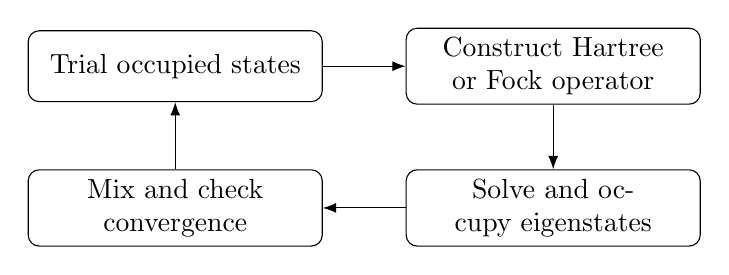
\begin{tikzpicture}[>=Latex,every node/.style={draw,rounded corners,align=center,text width=3.5cm,minimum height=0.9cm}]
\node (guess) at (0,0) {Trial occupied states};
\node (field) at (4.8,0) {Construct Hartree or Fock operator};
\node (solve) at (4.8,-1.8) {Solve and occupy eigenstates};
\node (check) at (0,-1.8) {Mix and check convergence};
\draw[->] (guess)--(field);\draw[->] (field)--(solve);
\draw[->] (solve)--(check);\draw[->] (check)--(guess);
\end{tikzpicture}
\end{center}

\section*{4. What DFT adds}
Ground-state density functional theory (DFT) makes the three-dimensional density the basic variable. Its exact universal functional contains both exchange and correlation, whereas ordinary HF restricts the state to a single determinant and omits the remaining correlation energy. Practical Kohn--Sham DFT introduces auxiliary orbitals to evaluate the noninteracting kinetic energy. With a local or semilocal exchange-correlation approximation, it avoids the full nonlocal Fock exchange operation and is often less expensive.

These are formal and computational advantages, not a guarantee that every approximate density functional is more accurate than HF. The exact functional is not generally available; approximate functionals can have self-interaction, band-gap, dispersion, or strong-correlation errors. Kohn--Sham DFT still solves for occupied orbitals and is not simply one scalar differential equation for the density.

\section*{5. Hohenberg--Kohn energy functional}
For fixed interaction and particle number, a precise universal functional can be written using a constrained search:
\[
F[n]=\min_{\Psi\to n}\bra{\Psi}\hat T+\hat W\ket{\Psi}.
\]
The minimization is over admissible antisymmetric many-electron states with density $n$. With an external potential $v_{\mathrm{ext}}$, the energy functional is
\[
\boxed{E_v[n]=F[n]+\int v_{\mathrm{ext}}(\vct r)n(\vct r)\dd^3r.}
\]
A fixed ion--ion energy may be added as a constant. The universal $F[n]$ does not explicitly depend on $v_{\mathrm{ext}}$; the full $E_v[n]$ does. Among admissible densities with $\int n=N$, the ground-state density minimizes $E_v[n]$ and gives the ground-state energy. Different external potentials normally produce different minimizing densities.

In the original nondegenerate Hohenberg--Kohn setting, the ground-state density determines the external potential up to an additive constant. The constrained-search formulation expresses the energy minimization without needing to assign every trial density to a unique nondegenerate external-potential ground state.

\section*{6. Kohn--Sham equations}
Decompose the universal functional as
\[
F[n]=T_s[n]+E_{\mathrm H}[n]+E_{\mathrm{xc}}[n],\qquad
E_{\mathrm H}[n]=\frac12\iint\frac{e^2n(\vct r)n(\vct r')}{|\vct r-\vct r'|}\dd^3r\dd^3r'.
\]
Here $T_s$ is the kinetic energy of an auxiliary noninteracting system with density $n$. The definition
\[
E_{\mathrm{xc}}[n]=F[n]-T_s[n]-E_{\mathrm H}[n]
\]
includes exchange, the interaction correlation beyond the Hartree term, and the difference between interacting and noninteracting kinetic energies.

For a spin-independent potential, the equations are
\begin{align*}
\left[-\frac{\hbar^2\nabla^2}{2m}+v_{\mathrm{ext}}(\vct r)
+v_{\mathrm H}(\vct r)+v_{\mathrm{xc}}(\vct r)\right]\phi_i(\vct r)
&=\epsilon_i\phi_i(\vct r),\\
n(\vct r)&=\sum_i f_i|\phi_i(\vct r)|^2,\\
v_{\mathrm H}(\vct r)&=\int\frac{e^2n(\vct r')}{|\vct r-\vct r'|}\dd^3r',\qquad
v_{\mathrm{xc}}(\vct r)=\frac{\delta E_{\mathrm{xc}}}{\delta n(\vct r)}.
\end{align*}
The occupations satisfy $\sum_i f_i=N$. They are at most two for spatial orbitals in a spin-degenerate treatment, or at most one for explicitly labelled spin orbitals. Spin-polarized calculations use $E_{\mathrm{xc}}[n_\uparrow,n_\downarrow]$ and a potential for each spin. Self-consistency is required because the potential is a functional of the density obtained from the orbitals.

\section*{7. Deriving Kohn--Sham from the energy functional}
Represent the density by orthonormal auxiliary orbitals and write
\[
T_s=-\sum_i f_i\int\phi_i^*\frac{\hbar^2\nabla^2}{2m}\phi_i\dd^3r.
\]
Vary $E_v[n]$ with respect to $\phi_i^*$ while constraining orbital orthonormality. Since $\delta n=f_i\phi_i\delta\phi_i^*$ for this variation,
\begin{align*}
\frac{\delta T_s}{\delta\phi_i^*}&=-f_i\frac{\hbar^2\nabla^2}{2m}\phi_i,\\
\frac{\delta(E_{\mathrm H}+E_{\mathrm{xc}}+\int vn)}{\delta\phi_i^*}
&=f_i(v_{\mathrm H}+v_{\mathrm{xc}}+v)\phi_i.
\end{align*}
The Euler--Lagrange equations are consequently the Kohn--Sham equations of Question 6, after diagonalizing the constraint matrix within equal-occupation subspaces. They are a way to minimize the density functional while treating $T_s$ through orbitals; the orbitals are not generally the exact interacting many-electron wavefunction.

An independent consistency check is the total-energy expression. Summing occupied Kohn--Sham eigenvalues counts the Hartree term twice and includes $\int nv_{\mathrm{xc}}$, rather than $E_{\mathrm{xc}}$. Thus
\[
\boxed{E=\sum_i f_i\epsilon_i-E_{\mathrm H}
-\int n v_{\mathrm{xc}}\dd^3r+E_{\mathrm{xc}}+E_{\mathrm{ion-ion}}.}
\]
The sum of eigenvalues alone is not the total energy.

\section*{8. Functional derivative in the LDA}
Because $\varepsilon_{\mathrm{xc}}(n)$ is an energy \emph{per electron}, the LDA functional is
\[
E_{\mathrm{xc}}^{\mathrm{LDA}}[n]=\int n(\vct r)\varepsilon_{\mathrm{xc}}(n(\vct r))\dd^3r.
\]
Under an arbitrary small density change,
\[
\delta E_{\mathrm{xc}}^{\mathrm{LDA}}
=\int\left[\varepsilon_{\mathrm{xc}}(n)+n\frac{\dd\varepsilon_{\mathrm{xc}}}{\dd n}\right]\delta n\dd^3r.
\]
Reading off the coefficient of $\delta n$ gives
\[
\boxed{v_{\mathrm{xc}}^{\mathrm{LDA}}(\vct r)
=\left.\left[\varepsilon_{\mathrm{xc}}(n)+n\varepsilon_{\mathrm{xc}}'(n)\right]\right|_{n=n(\vct r)}.}
\]
It is not merely $\varepsilon_{\mathrm{xc}}$, nor merely its derivative. For example, if $\varepsilon_x=-C n^{1/3}$, then $v_x=-(4C/3)n^{1/3}$. Consequently $\int n v_x=(4/3)E_x$, illustrating why the reference shortcut $E_{\mathrm{xc}}=\int n v_{\mathrm{xc}}$ is generally false.

\section*{9. Tight-binding Bloch sums}
Let $\vct R$ run over $N_c$ Bravais lattice sites, $\vct\tau_\alpha$ identify an atom in the primitive-cell basis, and $\varphi_{\alpha\mu}$ be a localized orbital. One convenient phase convention is
\[
\chi_{\alpha\mu,\vct k}(\vct r)=\frac1{\sqrt{N_c}}
\sum_{\vct R}\ee^{\ii\vct k\cdot(\vct R+\vct\tau_\alpha)}
\varphi_{\alpha\mu}(\vct r-\vct R-\vct\tau_\alpha).
\]
Translate by a Bravais vector $\vct T$ and substitute $\vct R'=\vct R-\vct T$. Then
\[
\chi_{\alpha\mu,\vct k}(\vct r+\vct T)
=\ee^{\ii\vct k\cdot\vct T}\chi_{\alpha\mu,\vct k}(\vct r),
\]
so each sum has the Bloch transformation law. An eigenstate is a linear combination of these sums at fixed $\vct k$:
\[
\psi_{n\vct k}=\sum_{\alpha\mu}c_{\alpha\mu,n}(\vct k)\chi_{\alpha\mu,\vct k}.
\]
Projection gives $H(\vct k)c_n=E_n(\vct k)S(\vct k)c_n$. Here $S$ is the orbital-overlap matrix. The displayed $1/\sqrt{N_c}$ yields individually normalized Bloch sums only when the localized basis is orthonormal, or its overlap is neglected; otherwise $S$ or explicit normalization must be retained. The hopping matrix elements, not dimensionless overlaps alone, determine the energy dispersion.

\section*{10. Silicon orbitals and band counting}
\textbf{(a) Five orbitals per atom.} Silicon has four chemically active valence orbitals, $3s$ and the three $3p$ orbitals. A common five-orbital empirical choice is
\[
\boxed{\{s,p_x,p_y,p_z,s^*\}.}
\]
The extra excited $s$-like orbital improves the description of the low conduction bands. It is an effective basis state, not a fifth occupied valence orbital in the isolated ground-state atom. Core $1s$, $2s$, and $2p$ states are normally excluded from this valence-band model.

\textbf{(b) Number of bands.} Diamond-structure silicon has two atoms per primitive cell. Five spatial orbitals on each atom produce a $10\times10$ Bloch Hamiltonian, hence $\boxed{10\text{ spatial bands}}$. With spin degeneracy, each band accommodates two electrons per primitive cell. Counting spin-resolved branches instead gives 20 coincident branches when spin splitting is absent. Using the eight atoms of the conventional cubic cell would fold the bands and change the bookkeeping, not create new physical states.

\textbf{(c) Filled bands.} There are $2\times4=8$ valence electrons per primitive cell. In the insulating ground state, each full spin-degenerate band holds two, so
\[
\boxed{N_{\mathrm{filled}}=\frac82=4.}
\]
The remaining six spatial bands in the model are unoccupied. Counting only one atom would incorrectly give two occupied bands.

\section*{11. Why bare plane waves converge slowly near cores}
A plane wave is smooth, but an all-electron valence state has rapid variations near nuclei and must be orthogonal to compact core states. Resolving these short length scales requires large reciprocal vectors $\vct G$ and a high kinetic-energy cutoff,
\[
\frac{\hbar^2|\vct k+\vct G|^2}{2m}\le E_{\mathrm{cut}}.
\]
In three dimensions the number of waves grows approximately as $E_{\mathrm{cut}}^{3/2}$. A finite plane-wave variational calculation that does not constrain the valence subspace can also approach lower core states. This is a failure to isolate the intended valence problem, not an unbounded-below nonrelativistic Hamiltonian.

Three related remedies are useful:
\begin{enumerate}
\item \textbf{Orthogonalized plane waves (OPW).} Project every plane wave out of the occupied core space: $(1-P_c)\ket{\vct k+\vct G}$. Core orthogonality is then built into the basis.
\item \textbf{Pseudopotentials.} Replace the strong core potential and nodal all-electron valence function by an effective potential and a smooth pseudo-wavefunction that reproduce the relevant valence scattering and external behavior. Fewer plane waves are needed.
\item \textbf{Augmentation methods.} Use an appropriate near-nucleus representation together with a smooth interstitial representation, as in augmented-wave approaches.
\end{enumerate}
If $\ket{\psi}=(1-P_c)\ket{\phi}$ and $H\ket{\chi_c}=\epsilon_c\ket{\chi_c}$, the OPW construction implies
\[
\left[H+\sum_c(E-\epsilon_c)\ket{\chi_c}\bra{\chi_c}\right]\ket{\phi}=E\ket{\phi}.
\]
For a valence state above the core energies, the additional projector term is repulsive. This is the Phillips--Kleinman connection between core orthogonality and an effective pseudopotential.

\section*{12. Core Bloch sums for LiH}
In the usual rocksalt description, a primitive cell contains one Li and one H. The standard valence partition freezes the tightly bound Li $1s^2$ shell as core; Li $2s$ and H $1s$ contribute to the valence sector. Although the occupied valence states have substantial H character, H $1s$ is not an additional frozen core in this partition.

For Li sites $\vct R+\vct\tau_{\mathrm{Li}}$, the spatial core Bloch sum is
\[
\boxed{\chi_{c\vct k}(\vct r)=\mathcal N_{\vct k}\sum_{\vct R}
\ee^{\ii\vct k\cdot(\vct R+\vct\tau_{\mathrm{Li}})}
\varphi_{\mathrm{Li},1s}(\vct r-\vct R-\vct\tau_{\mathrm{Li}}).}
\]
There is one such spatial core band, doubly occupied when spin is included. If intersite core overlap is negligible, $\mathcal N_{\vct k}=1/\sqrt{N_c}$; otherwise normalize the sum or orthonormalize the core subspace. For each spin, the OPW is
\[
\ket{w_{\vct k+\vct G}}=\ket{\vct k+\vct G}
-\ket{\chi_{c\vct k}}\braket{\chi_{c\vct k}}{\vct k+\vct G}.
\]
Only a core Bloch sum at the same crystal momentum enters because different Bloch sectors are orthogonal. A different chosen frozen-core partition must be specified explicitly before changing the projector.

\section*{Primary references and checks}
The algebra is derived above. The following original papers establish the functional and basis constructions used for comparison:
\begin{itemize}
\item P. Hohenberg and W. Kohn, \href{https://doi.org/10.1103/PhysRev.136.B864}{\textit{Inhomogeneous Electron Gas} (1964)}.
\item W. Kohn and L. J. Sham, \href{https://doi.org/10.1103/PhysRev.140.A1133}{\textit{Self-Consistent Equations Including Exchange and Correlation Effects} (1965)}.
\item J. C. Phillips and L. Kleinman, \href{https://doi.org/10.1103/PhysRev.116.287}{\textit{New Method for Calculating Wave Functions in Crystals and Molecules} (1959)}.
\item P. Vogl, H. P. Hjalmarson, and J. D. Dow, \href{https://doi.org/10.1016/0022-3697(83)90064-1}{\textit{A Semi-empirical Tight-binding Theory of the Electronic Structure of Semiconductors} (1983)}.
\end{itemize}

\chapter{Solid State Theory: April 23, 2021 --- Solutions}
\label{s:theory-2021-04-midterm}
\begin{sourceNote}
These are independent solutions, not an official answer key. Several true/false statements require a convention or a qualification; those conditions are stated rather than hidden. Reciprocal vectors use $\mathbf g_i\cdot\mathbf t_j=2\pi\delta_{ij}$.
\end{sourceNote}

\section*{1. True/false, with reasons and necessary qualifications}
\subsection*{(a) Diamond sites form a Bravais lattice: false}
Diamond consists of an FCC Bravais lattice with a two-atom basis, for example $\mathbf d_1=0$, $\mathbf d_2=(a/4)(1,1,1)$. Translating by $\mathbf d_2$ sends the first atom to the second but does not map the entire crystal to itself: twice that displacement is not a diamond site relative to the chosen origin. The carbon sites are therefore not a one-site Bravais lattice.

\subsection*{(b) The two vector pairs span the same lattice: false}
The primitive parallelogram areas would be
\[
|\det(\mathbf t_1,\mathbf t_2)|=|2ab-ab|=ab,\qquad
|\det(\mathbf s_1,\mathbf s_2)|=|-ab+6ab|=5ab.
\]
More explicitly,
\[
\mathbf s_1=4\mathbf t_1+7\mathbf t_2,\qquad
\mathbf s_2=-3\mathbf t_1-4\mathbf t_2,
\quad
M=\begin{pmatrix}4&-3\\7&-4\end{pmatrix},\quad\det M=5.
\]
An integer basis change preserves a lattice only if its determinant is $\pm1$. Here the $\mathbf s$ vectors generate an index-5 sublattice of the $\mathbf t$ lattice, with only one fifth as many sites per unit area.

\subsection*{(c) Same point group implies same crystal system: true}
With point group understood as the full crystallographic point group, two Bravais lattices with that same group belong to the same crystal system. They may differ in centering. For example, primitive, body-centered, and face-centered cubic Bravais lattices are distinct but all belong to the cubic system. Sharing merely a subgroup, such as inversion alone, would not suffice.

\subsection*{(d) Same species implies a Bravais translation: false in general}
Positions have the form $\mathbf R+\mathbf d_\alpha$. The difference of two positions is a Bravais vector only if their basis-site difference is also a Bravais vector. Diamond supplies two carbon atoms whose separation $(a/4)(1,1,1)$ is not an FCC translation.
The phrase \emph{simple crystal} is not defined in the question. If it is explicitly defined in a course as a one-atom Bravais crystal, the statement is true by that extra definition. Chemical purity or a perfect defect-free crystal alone does not establish it.

\subsection*{(e) Wigner-Seitz and Brillouin-zone product: true for volumes}
The meaningful interpretation is the product of their volumes. Write the direct and reciprocal basis matrices as $T$ and $G=2\pi T^{-T}$. Then
\[
\Omega=|\det T|,\qquad
\Omega^*=|\det G|=\frac{(2\pi)^3}{\Omega},\qquad
\boxed{\Omega\Omega^*=(2\pi)^3.}
\]
Wigner-Seitz cells have the same volume as the corresponding primitive parallelepipeds. The constant depends on the reciprocal-vector convention; it would be 1 if the $2\pi$ were omitted throughout.

\subsection*{(f) Allowed $\mathbf k$-point density scales with volume: true}
For $N_i$ cells along each primitive direction, Born-von Karman conditions give
\[
\mathbf k=\sum_i\frac{m_i}{N_i}\mathbf g_i,
\qquad m_i=0,\ldots,N_i-1.
\]
There are $N_c=N_1N_2N_3$ inequivalent points per Brillouin zone. If the sample volume is $V=N_c\Omega$, each point occupies reciprocal volume $(2\pi)^3/V$ and
\[
\boxed{\frac{\dd N_k}{\dd^3k}=\frac{V}{(2\pi)^3}.}
\]
This counts wavevectors; each band and spin supplies additional electronic states. Increasing the sample volume makes the $k$ mesh denser, not sparser.

\subsection*{(g) One cell determines a Bloch eigenstate elsewhere: true}
For a chosen Bloch state,
\[
\psi_{n\mathbf k}(\mathbf r+\mathbf R)=
\ee^{\ii\mathbf k\cdot\mathbf R}\psi_{n\mathbf k}(\mathbf r).
\]
Knowing the wavefunction within one cell and its $\mathbf k$ therefore determines it in every translated cell. The qualification is that a Bloch eigenbasis is chosen: arbitrary linear combinations of degenerate states with different $\mathbf k$ need not possess a single translation phase.

\subsection*{(h) HF energy must be strictly lower than Hartree: qualified}
As an unconditional assertion of a \emph{strict} inequality, the statement is false. The standard negative-exchange argument compares a fixed orthonormal orbital set:
\[
E_{\rm HF}-E_{\rm Hartree\ product}
=-\frac12\sum_{i\ne j}K_{ij}\leq0,
\]
Here $x=(\mathbf r,\sigma)$ includes spin, integration over $x$ includes the spin sum, and $w(\mathbf r-\mathbf r')=e^2/(4\pi\varepsilon_0|\mathbf r-\mathbf r'|)$. The exchange integral is
\[
K_{ij}=\int\dd x\dd x'\,
\chi_i^*(x)\chi_j(x)w(\mathbf r-\mathbf r')\chi_j^*(x')\chi_i(x')\geq0.
\]
Thus exchange lowers or leaves unchanged that reference energy. Opposite-spin pairs have zero exchange, and equality is possible when all relevant off-diagonal exchange integrals vanish. A strict decrease needs at least one nonzero such integral. Separately optimized Hartree products and HF determinants also have different variational constraints; a universal ordering cannot be inferred simply by calling one wavefunction antisymmetric. Under the usual classroom fixed-orbital comparison with nonzero exchange, the intended lower-energy conclusion holds with these qualifications.

\subsection*{(i) A self-consistent HF determinant is an exact eigenfunction: false}
HF makes the energy stationary under variations within the single-determinant manifold. The interacting Hamiltonian can couple that determinant to excited determinants, especially double excitations. In general,
$\hat H\Phi_{\rm HF}\neq E\Phi_{\rm HF}$.
An exact single-determinant eigenstate is a special case, not a consequence of solving the HF equations.

\subsection*{(j) A self-consistent HF determinant is the best many-body state: false as written}
The variational minimum satisfies
\[
E_0\leq\min_{\Phi\ {\rm single\ determinant}}\langle\Phi|\hat H|\Phi\rangle
=E_{\rm HF}^{\min}.
\]
Correlated wavefunctions outside this restricted class can lower the energy. Moreover, a solution of the HF equations can be a local minimum or another stationary point, rather than the global determinant minimum. The precise valid claim is: \emph{the globally minimizing HF determinant is the best energy approximation within the class of allowed single determinants}. It need not be the best wavefunction among all many-electron states.

\subsection*{(k) The unpolarized homogeneous gas always has lower energy: false}
Interpret the normal state as the unpolarized uniform state. The competition depends on density: polarization increases Fermi kinetic energy but makes exchange more negative. This is explicit in the uniform Hartree-Fock model. In atomic units, let
\[
k_F=(3\pi^2n)^{1/3}=\frac{c_0}{r_s},\quad
c_0=(9\pi/4)^{1/3},\quad
\zeta=\frac{n_\uparrow-n_\downarrow}{n}.
\]
With the positive background canceling the uniform Hartree term, the energy per electron is
\[
e_{\rm HF}(\zeta)=
\frac{3k_F^2}{20}\big[(1+\zeta)^{5/3}+(1-\zeta)^{5/3}\big]
-\frac{3k_F}{8\pi}\big[(1+\zeta)^{4/3}+(1-\zeta)^{4/3}\big].
\]
The powers follow from each spin Fermi sphere: kinetic energy density scales as $n_\sigma^{5/3}$ and exchange as $-n_\sigma^{4/3}$. Comparing $\zeta=1$ with $\zeta=0$ gives
\[
\Delta e=\frac{3k_F^2}{10}(2^{2/3}-1)
-\frac{3k_F}{4\pi}(2^{1/3}-1).
\]
At high density the first term wins; at lower density the second can win. These two uniform HF branches cross at
\[
r_s^*=\frac{2\pi c_0}{5}(2^{1/3}+1)\simeq5.45.
\]
This example concerns uniform HF states; it is not a claim that this is the exact phase boundary of the correlated electron gas. Correlation and other possible ordered states require separate treatment. There is no density-independent energy-ordering theorem of the asserted form.

\subsection*{(l) Electron density depends on external potential: true for the physical density}
For a fixed electron number and interaction, the physical density is the minimizer
\[
n_0[v]=\mathop{\rm arg\,min}_n\left(F[n]+\int v(\mathbf r)n(\mathbf r)\,\dd^3r\right).
\]
Changing $v$ generally changes $n_0$. What is universal is $F[n]$: it has no \emph{explicit} dependence on the external potential. A trial density used in the variation is an independent argument. Confusing that functional argument with the resulting minimizing density leads to the wrong conclusion.

\subsection*{(m) KS orbitals form the interacting ground-state determinant: false}
KS orbitals define an auxiliary noninteracting state chosen to reproduce the interacting ground-state \emph{density}. Its Slater determinant is generally not the interacting many-electron wavefunction. Matching a one-body density does not reproduce all pair correlations or all expectation values.

\subsection*{(n) Both density and interacting kinetic energy are KS sums: false}
With exact KS orbitals and the appropriate occupations,
\[
n_0(\mathbf r)=\sum_i f_i|\phi_i(\mathbf r)|^2
\]
is correct. But
\[
T_s=\sum_i f_i\left\langle\phi_i\left|\frac{\mathbf p^2}{2m}\right|\phi_i\right\rangle
\]
is the auxiliary noninteracting kinetic energy, not in general the interacting $T$. The kinetic correlation contribution $T-T_s$ is part of $E_{xc}$. A conjunction is false when its second assertion fails.

\subsection*{(o) KS gives the exact density and energy: true only in the exact theory}
With the exact exchange-correlation functional, an appropriate KS representation, and the ground-state self-consistent solution, the formal theory yields the exact density and ground-state electronic energy:
\[
E_0=T_s[n_0]+E_H[n_0]+E_{xc}[n_0]+\int v_{\rm ext}n_0\,\dd^3r.
\]
This does not make practical LDA or other approximate functionals exact. Nor does it identify every KS eigenvalue with a physical excitation energy. The intended formal-theory answer is true; the unconditional assertion about all numerical KS calculations would be false.

\section*{2. Hamiltonian and density-functional terminology}
\subsection*{(a) Fixed-nuclei many-electron Hamiltonian}
For nuclei of charge $Z_Ae$ at fixed positions $\mathbf R_A$,
\begin{align*}
\hat H_e&=\sum_{i=1}^N\left[-\frac{\hbar^2}{2m}\nabla_i^2
-\sum_A\frac{Z_Ae^2}{4\pi\varepsilon_0|\mathbf r_i-\mathbf R_A|}\right]
+\sum_{i<j}\frac{e^2}{4\pi\varepsilon_0|\mathbf r_i-\mathbf r_j|},\\
E_{NN}&=\sum_{A<B}\frac{Z_AZ_Be^2}{4\pi\varepsilon_0|\mathbf R_A-\mathbf R_B|}.
\end{align*}
The three electronic terms are kinetic energy, electron-nucleus attraction, and electron-electron repulsion. The full fixed-configuration energy includes the constant $E_{NN}$. Nuclear kinetic energy is absent because the nuclei are held fixed. The $i<j$ and $A<B$ restrictions count each pair once. Other applied external potentials can be added to the one-electron potential. The electronic wavefunction must be antisymmetric in electron space-spin coordinates.

\subsection*{(b) Hohenberg-Kohn functional}
The universal interacting functional can be expressed by constrained search:
\[
F[n]=\min_{\Psi\to n}\langle\Psi|\hat T+\hat W_{ee}|\Psi\rangle.
\]
For a specified external potential,
\[
E_v[n]=F[n]+\int v(\mathbf r)n(\mathbf r)\,\dd^3r,
\qquad E_0=\min_{n\ {
m admissible},\,\int n=N}E_v[n].
\]
The first HK theorem relates ground-state density to external potential, up to an additive constant under its usual assumptions; the second establishes the density variational principle. $F$ is independent of which fixed nuclear configuration produces $v$, while its minimizing density is not.

\subsection*{(c) Exchange-correlation functional}
Define the noninteracting kinetic functional $T_s[n]$ and classical Coulomb functional
\[
E_H[n]=\frac12\int\dd^3r\dd^3r'\,
\frac{e^2n(\mathbf r)n(\mathbf r')}{4\pi\varepsilon_0|\mathbf r-\mathbf r'|}.
\]
Then
\[
\boxed{E_{xc}[n]=F[n]-T_s[n]-E_H[n]
=(T[n]-T_s[n])+(W_{ee}[n]-E_H[n]).}
\]
The second expression refers to the constrained-search minimizing interacting state. Exchange, correlation beyond classical Coulomb repulsion, self-interaction cancellation, and the kinetic correction are included. The potential entering the KS equation is $v_{xc}(\mathbf r)=\delta E_{xc}/\delta n(\mathbf r)$.

\subsection*{(d) Local density approximation}
LDA uses the exchange-correlation energy per electron of a uniform gas at the local density:
\[
\boxed{E_{xc}^{\rm LDA}[n]=\int n(\mathbf r)
\varepsilon_{xc}^{\rm unif}(n(\mathbf r))\,\dd^3r.}
\]
Its potential is $v_{xc}^{\rm LDA}=\varepsilon_{xc}^{\rm unif}+n\,\dd\varepsilon_{xc}^{\rm unif}/\dd n$, evaluated at the local $n$. It is local in the density and omits explicit gradients and nonlocal correlations. It is motivated by a locally uniform or slowly varying density, rather than by an assumption that all real crystals have uniform charge density.

\section*{3. FCC lattice and the plane perpendicular to a body diagonal}
\subsection*{(a) Primitive volume and lattice-point density}
A conventional cubic cell contains $8(1/8)+6(1/2)=4$ FCC lattice points, so
\[
\boxed{\Omega=\frac{a^3}{4},\qquad \rho_{\rm lattice}=\frac4{a^3}.}
\]
This is a lattice-point density; a separate multi-atom basis would change atom density, not the Bravais-point density.

\subsection*{(b) Direct and reciprocal primitive vectors}
Choose
\[
\mathbf t_1=\frac a2(0,1,1),\quad
\mathbf t_2=\frac a2(1,0,1),\quad
\mathbf t_3=\frac a2(1,1,0).
\]
Using $\mathbf g_1=2\pi(\mathbf t_2\times\mathbf t_3)/\Omega$ and cyclic permutations gives
\[
\boxed{\mathbf g_1=\frac{2\pi}{a}(-1,1,1),\quad
\mathbf g_2=\frac{2\pi}{a}(1,-1,1),\quad
\mathbf g_3=\frac{2\pi}{a}(1,1,-1).}
\]
Their dot products with the $\mathbf t_j$ verify the reciprocal relation. The reciprocal lattice is BCC, with conventional cubic lattice constant $4\pi/a$.

\subsection*{(c) A (111) layer is a triangular lattice}
Take the normal along $(1,1,1)$. A basis in a layer is
\[
\mathbf u=\mathbf t_2-\mathbf t_1=\frac a2(1,-1,0),\qquad
\mathbf v=\mathbf t_3-\mathbf t_1=\frac a2(1,0,-1).
\]
Both dot products with $(1,1,1)$ vanish. Their lengths are $a/\sqrt2$ and $\mathbf u\cdot\mathbf v=a^2/4$, hence their angle is $60^\circ$. They span a two-dimensional triangular, or two-dimensional hexagonal Bravais, lattice. Its primitive area and planar density are
\[
\boxed{A_{111}=\frac{\sqrt3a^2}{4},\qquad
\sigma_{111}=\frac4{\sqrt3a^2}.}
\]
The shortest reciprocal normal is $(2\pi/a)(1,1,1)$, so adjacent lattice layers are separated by $a/\sqrt3$; indeed $A_{111}(a/\sqrt3)=a^3/4$. The triangular lattice of one plane should not be confused with the three-dimensional hexagonal lattice. Consecutive FCC (111) layers have the familiar ABC offsets.

\begin{center}
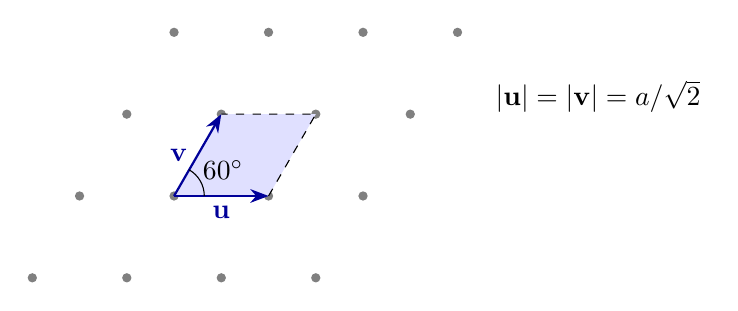
\begin{tikzpicture}[scale=1.2,>=Stealth]
\foreach \i in {-1,0,1,2}{\foreach \j in {-1,0,1,2}{
\fill[gray] ({\i+\j/2},{.8660254*\j}) circle(1.4pt);}}
\fill[blue!12] (0,0)--(1,0)--(1.5,.8660254)--(.5,.8660254)--cycle;
\draw[thick,blue!60!black,->] (0,0)--(1,0) node[midway,below] {$\mathbf u$};
\draw[thick,blue!60!black,->] (0,0)--(.5,.8660254) node[midway,left] {$\mathbf v$};
\draw[dashed] (1,0)--(1.5,.8660254)--(.5,.8660254);
\draw (.32,0) arc (0:60:.32);
\node at (.52,.27) {$60^\circ$};
\node[anchor=west] at (3.3,1.05) {$|\mathbf u|=|\mathbf v|=a/\sqrt2$};
\end{tikzpicture}
\end{center}

\section*{4. Honeycomb reciprocal lattice, critical points, and DOS}
\subsection*{(a) Reciprocal primitive vectors}
The direct-cell area is $A_c=\sqrt3a^2/2$. Solving
$\mathbf g_i\cdot\mathbf t_j=2\pi\delta_{ij}$ gives
\[
\boxed{\mathbf g_1=\frac{2\pi}{a}(1,1/\sqrt3),\qquad
\mathbf g_2=\frac{2\pi}{a}(-1,1/\sqrt3).}
\]
For example, the two equations for $\mathbf g_1$ are
$ag_{1x}/2+\sqrt3ag_{1y}/2=2\pi$ and
$-ag_{1x}/2+\sqrt3ag_{1y}/2=0$.
The reciprocal primitive area is $8\pi^2/(\sqrt3a^2)$, and its product with $A_c$ is $(2\pi)^2$.

\subsection*{(b) Classifying $\Gamma$, $Q$, and $P$}
Set $x=ak_x$, $y=ak_y$, and $h=|F|^2$. Direct differentiation yields
\[
h_x=-2\sin(x/2)\cos(\sqrt3y/2)-4\cos(x/2)\sin(x/2),\qquad
h_y=-2\sqrt3\cos(x/2)\sin(\sqrt3y/2).
\]
For $h>0$, a band is stationary exactly when $\nabla h=0$.

At $\Gamma$, $h=9$ and, for displacement $\mathbf q$,
\[
|F|=3-\frac{a^2q^2}{4}+O(a^4q^4),\qquad
\epsilon_\pm=\epsilon_p\pm3\gamma\mp\frac{\gamma a^2q^2}{4}+O(q^4).
\]
Thus the upper band has a smooth maximum and the lower band a smooth minimum, with Hessians $\mp(\gamma a^2/2)I$.

At $Q$, $h=1$ and the dimensionless Hessian is
\[
H_h(Q)=\begin{pmatrix}2&\sqrt3\\\sqrt3&0\end{pmatrix}.
\]
Its eigenvectors can be chosen as $(\sqrt3/2,1/2)$ and $(-1/2,\sqrt3/2)$, with eigenvalues $3,-1$. In their displacement coordinates $u,v$,
\[
|F|=1+\frac{a^2}{4}(3u^2-v^2)+O(a^3q^3),\qquad
\epsilon_\pm=\epsilon_p\pm\gamma\pm\frac{\gamma a^2}{4}(3u^2-v^2)+O(a^3q^3).
\]
Each band has a saddle. In the original coordinates the quadratic correction to $|F|$ is
$a^2q_x^2/2+\sqrt3a^2q_xq_y/2$, so dropping the mixed term would give an incorrect classification.

At $P$, $h=0$, and
\[
h=\frac{3a^2q^2}{4}+O(a^3q^3),\qquad
\epsilon_\pm=\epsilon_p\pm\frac{\sqrt3\gamma a}{2}|\mathbf q|+O(q^2).
\]
This is a Dirac contact: a conical minimum in the upper band and a conical maximum in the lower band. The individual energy-ordered bands are not differentiable at the vertex, so there is no ordinary stationary gradient or quadratic Hessian there. Under a broader definition it is a band-contact critical singularity, not a smooth Morse critical point. Its one-sided directional slopes are finite.

\subsection*{(c) Choosing $Q$: derivation of the logarithmic DOS}
For the upper band near one $Q$, define
\[
E_Q=\epsilon_p+\gamma,\quad e=E-E_Q,\quad
\alpha=\frac{3\gamma a^2}{4},\quad\beta=\frac{\gamma a^2}{4},\quad
\epsilon-E_Q\simeq\alpha u^2-\beta v^2.
\]
The DOS per unit sample area per spin from that patch is
\[
g_Q(E)=\frac1{(2\pi)^2}\int_{\rm patch}\dd u\dd v\,
\delta(e-\alpha u^2+\beta v^2).
\]
Let $X=\sqrt\alpha u$, $Y=\sqrt\beta v$, then $U=X+Y$, $V=X-Y$. The energy becomes $UV$ and
$\dd u\dd v=\dd U\dd V/(2\sqrt{\alpha\beta})$.
Choose a small cutoff patch $|U|,|V|<L$. For $0<|e|<L^2$, integration over $V$ gives $1/|U|$ only when $|U|>|e|/L$. Hence
\begin{align*}
g_Q(E)&\simeq\frac1{8\pi^2\sqrt{\alpha\beta}}
\int_{|e|/L<|U|<L}\frac{\dd U}{|U|}\\
&=\frac1{4\pi^2\sqrt{\alpha\beta}}\log\frac{L^2}{|e|}\\
&=\boxed{\frac1{\pi^2\sqrt3\gamma a^2}
\log\frac{E_c}{|E-E_Q|},\qquad E_c=L^2.}
\end{align*}
The coefficient of the logarithm is fixed by the local curvatures. The cutoff scale and nonsingular background depend on the chosen patch and higher-order terms. The lower-band saddle has the same singular coefficient about $E_Q=\epsilon_p-\gamma$.

This counts a single saddle patch and one spin. Multiply by spin or distinct-saddle multiplicities only when summing those contributions, and multiply by $A_c$ for DOS per cell. A patch centered on a zone edge is understood on the reciprocal-space torus, or split and translated into the first zone; it must not be counted twice. The logarithmic saddle singularity differs from the constant step at $\Gamma$ and from the linear, vanishing DOS at a Dirac point.

\section*{Primary references and verification scope}
The calculations of reciprocal vectors, Hessians, and local DOS are derived from the question's formulas. For the model and density-functional foundations, see
\href{https://doi.org/10.1103/PhysRev.71.622}{Wallace, The Band Theory of Graphite (1947)},
\href{https://doi.org/10.1103/PhysRev.136.B864}{Hohenberg and Kohn, Inhomogeneous Electron Gas (1964)},
and
\href{https://doi.org/10.1103/PhysRev.140.A1133}{Kohn and Sham, Self-Consistent Equations Including Exchange and Correlation Effects (1965)}.
The polarized-gas comparison is explicitly a uniform Hartree-Fock calculation and is not presented as an exact correlated phase diagram.

\chapter{Solid State Theory: Midterm II, May 11, 2026}
\label{s:theory-2026-05-midterm-ii}
\begin{sourceNote}
These solutions are independently derived and checked against the supplied answers. The small Evjen cell gives an approximation, radius rules require a structural model, the ionic charge-transfer estimate must be distinguished from an unbound-pair gap, and the conducting dielectric function requires care at zero frequency. The original answer PDF is not reproduced.
\end{sourceNote}
Throughout this chapter set $C=e^2/(4\pi\varepsilon_0)$ in SI units. The question's shorthand $e^2/R$ therefore means $C/R$. Ions are taken to have charges $\pm e$ in the simple 1:1 ionic model. The time convention for response functions is $\ee^{-\ii\omega t}$, with damping rate $\gamma>0$.

\section*{1. Evjen boundary weights}
For NaCl the nearest unlike-ion distance is $R_0=a/2$. Center the specified cube on a reference ion and write the surrounding sites as
\[
\vct r=R_0(i,j,k),\qquad i,j,k\in\{-1,0,1\}.
\]
Signs alternate with $i+j+k$. In an Evjen sum, an ion on a face has weight $1/2$, one on an edge has weight $1/4$, and one at a corner has weight $1/8$. These sharing factors make the complete weighted cell electrically neutral when the central ion is included.

Taking the central ion to be positive, unlike ions contribute positively to the conventional positive Madelung constant. The shells inside this cube are
\begin{center}
\begin{tabular}{lllll}
\toprule
Position & Distance & Number & Weight & Signed total\\
\midrule
Face centers & $R_0$ & 6 & $1/2$ & $+3$\\
Edge centers & $\sqrt2R_0$ & 12 & $1/4$ & $-3$\\
Corners & $\sqrt3R_0$ & 8 & $1/8$ & $+1$\\
Outside this cube & $2R_0$ & 0 & --- & $0$\\
\bottomrule
\end{tabular}
\end{center}
The reference ion is excluded from its own potential. Thus
\[
\boxed{(n_1,n_2,n_3,n_4)=(3,-3,1,0)},\qquad
\boxed{\alpha_M^{\rm Evjen}=3-\frac3{\sqrt2}+\frac1{\sqrt3}\simeq1.45603.}
\]
The weighted charge check is $1-3+3-1=0$. The absence of the $2R_0$ shell follows from the specified cube size, not from a cancellation of six full second-axis neighbors. This smallest Evjen cell is quite crude: the converged NaCl value is about $1.74756$. Enlarging the neutral weighted cube, rather than interpreting the first result as exact, improves the estimate.

\section*{2. What radius ratios do and do not determine}
\subsection*{(a) Equal radii in the elementary ionic model}
Assume a 1:1 salt with unlike ions in contact and compare common structures using their Madelung energies. Both CsCl and NaCl can attain the same nearest unlike-ion distance
\[
R=R_A+R_C=2R_A.
\]
Their Madelung constants, with this nearest-distance normalization, are approximately
\[
\alpha_{\rm CsCl}=1.76267,\qquad \alpha_{\rm NaCl}=1.74756.
\]
At equal $R$, $-\alpha C/R$ is slightly more negative for CsCl, which provides eight unlike nearest neighbors rather than six. The expected answer in this model is therefore
\[
\boxed{\text{CsCl structure, within the stated hard-sphere/Madelung comparison}.}
\]
Equal radii alone do not determine the stable structure of every real material. Short-range repulsion, stoichiometry, covalency, pressure, and entropy can change the comparison. The radius argument is a model-based tendency, not a universal structure theorem.

\subsection*{(b) Exceeding the contact threshold does not forbid CsCl}
Put $r=R_A/R_C>1$ and let $a_c$ be the CsCl cubic edge. The nearest unlike-ion distance is $R=\sqrt3a_c/2$. Like ions on the corner simple-cubic sublattice must not overlap, so $a_c\ge2R_A$; the other sublattice similarly requires $a_c\ge2R_C$. Together with the unlike-ion constraint,
\[
R_{\rm CsCl}^{\min}=\max(R_A+R_C,\sqrt3R_A,\sqrt3R_C).
\]
Unlike ions can remain in contact only if
\[
R_A+R_C\ge\sqrt3R_A
\quad\Longleftrightarrow\quad
r\le\frac1{\sqrt3-1}=\frac{\sqrt3+1}{2}.
\]
When $r$ exceeds this threshold, the CsCl arrangement is still geometrically possible: it expands to $R=\sqrt3R_A>R_A+R_C$. What is lost is unlike-ion contact at the minimum nonoverlapping cell size.

There is even a small interval just above the threshold where its larger Madelung constant can compensate for the larger separation. In NaCl,
\[
R_{\rm NaCl}^{\min}=\max(R_A+R_C,\sqrt2R_A,\sqrt2R_C),
\]
so near the CsCl threshold the NaCl separation remains $R_A+R_C$. Comparing only Coulomb energies gives the CsCl preference when
\[
\frac{\alpha_{\rm CsCl}}{\sqrt3r}>
\frac{\alpha_{\rm NaCl}}{r+1}
\quad\Longleftrightarrow\quad
r<\frac{\alpha_{\rm CsCl}}
{\sqrt3\alpha_{\rm NaCl}-\alpha_{\rm CsCl}}\simeq1.394.
\]
Since $(\sqrt3+1)/2\simeq1.366$, this supplies an explicit model example with a ratio greater than the threshold. The answer to ``is it possible?'' is \textbf{yes}; it is not a claim that CsCl is favored for every larger ratio or after all energetic contributions are included.

\section*{3. Cohesion, bulk modulus, and an ionic excitation estimate}
\subsection*{(a) Born--Land\'e power-law model and energy reference}
For $N$ ion pairs, define the signed energy per pair relative to infinitely separated free ions:
\[
\boxed{u(R)=\frac{U(R)}N=\frac{\lambda}{R^n}-\frac{\alpha_M C}{R},
\qquad \lambda>0,\quad n>1.}
\]
The first term represents short-range repulsion and the second the electrostatic Madelung attraction. At equilibrium $E_{\rm coh}=u(R_0)<0$ in this convention. If ``cohesive energy'' is instead tabulated as a positive dissociation energy, use $D=-E_{\rm coh}>0$. An energy relative to free neutral atoms differs by the ionization/electron-affinity terms and cannot be substituted without converting the reference.

Setting $u'(R_0)=0$ gives
\[
-\frac{n\lambda}{R_0^{n+1}}+\frac{\alpha_M C}{R_0^2}=0,
\qquad
\lambda=\frac{\alpha_M C}{n}R_0^{n-1}.
\]
With $E_M=-\alpha_M C/R_0<0$,
\[
u(R)=E_M\left[\frac{R_0}{R}-\frac1n
\left(\frac{R_0}{R}\right)^n\right],\qquad
\boxed{E_{\rm coh}=E_M\left(1-\frac1n\right).}
\]

\subsection*{(b) Eliminate the empirical parameters}
A conventional NaCl cube has edge $2R$ and contains four ion pairs. Thus the volume per pair is $v=V/N=(2R)^3/4=2R^3$. Pressure and bulk modulus follow from energy derivatives at fixed $N$:
\[
P=-\frac{\dd u}{\dd v}=-\frac{u'(R)}{6R^2},\qquad
B=-v\frac{\dd P}{\dd v}=v\frac{\dd^2u}{\dd v^2}.
\]
Because $u'(R_0)=0$ and $\dd v/\dd R=6R^2$,
\[
B_0=\frac{u''(R_0)}{18R_0}.
\]
Differentiating the pair energy twice and using the equilibrium relation yields
\[
u''(R_0)=\frac{(n-1)\alpha_M C}{R_0^3}
=-\frac{(n-1)E_M}{R_0^2},
\qquad
B_0=-\frac{(n-1)E_M}{18R_0^3}.
\]
The cohesive-energy relation determines
\[
n=\frac{E_M}{E_M-E_{\rm coh}},\qquad
n-1=\frac{E_{\rm coh}}{E_M-E_{\rm coh}}.
\]
Consequently
\[
\boxed{B_0=\frac{E_M E_{\rm coh}}
{18R_0^3(E_{\rm coh}-E_M)}.}
\]
For the positive dissociation convention this is
\[
\boxed{B_0=\frac{|E_M|D}{18R_0^3(|E_M|-D)},\qquad 0<D<|E_M|.}
\]
Both forms are positive for the stable model and have units of energy per volume. The result assumes the same power-law model and energy reference used in part (a); it is not a model-independent inference from two measured quantities.

\subsection*{(c) Distinguish a separated pair from a bound charge-transfer pair}
Write $A=\Delta(\mathrm{Cl}^-)>0$ for the electron affinity of neutral Cl, equivalently the electron detachment energy of isolated Cl$^-$, and $I=\Delta(\mathrm{Na})>0$ for the ionization energy of neutral Na. Transferring an electron from Cl$^-$ to Na$^+$ costs $A-I$ in the isolated-ion bookkeeping: detachment costs $A$, while attachment to Na$^+$ releases $I$.

At either lattice site, removing one unit of favorable ionic charge costs $\alpha_M C/R_0$. Creating well-separated electron and hole defects therefore has the rigid-ion estimate
\[
\boxed{E_{\rm separated}\approx A-I+\frac{2\alpha_M C}{R_0}.}
\]
If the transfer instead creates a neighboring electron--hole pair, their mutual attraction lowers the energy by $C/R_0$:
\[
\boxed{E_{\rm CT}\approx A-I+\frac{(2\alpha_M-1)C}{R_0}.}
\]
This is the expression given as $\varepsilon_G$ in the supplied answer. It includes a nearest-neighbor binding correction. It is therefore best identified as a localized charge-transfer or excitonic excitation estimate, rather than automatically equated with the unbound electron--hole continuum gap. More generally the same rigid-ion argument for pair separation $d$ gives
\[
E(d)\approx A-I+\frac{2\alpha_M C}{R_0}-\frac C d.
\]
The distinction follows directly from the cross term in the electrostatic energy of the two changed site charges. Electronic polarization, lattice relaxation, screening of their attraction, and band dispersion are omitted by this simple model. No numerical gap is determined because no numerical values of $A,I,R_0$ are supplied.

\section*{4. Recovering the continuum gap from two exciton levels}
Assume the two peaks are the $n=1$ and $n=2$ members of one three-dimensional hydrogenic exciton series. With continuum band gap $E_g$ and ground-state binding energy $E_B>0$,
\[
\Delta_n=E_g-\frac{E_B}{n^2},\qquad
\Delta_1=E_g-E_B,\quad \Delta_2=E_g-\frac{E_B}{4}.
\]
Subtracting gives $\Delta_2-\Delta_1=3E_B/4$. Therefore
\[
\boxed{E_B=\frac43(\Delta_2-\Delta_1)},\qquad
\boxed{E_g=\frac{4\Delta_2-\Delta_1}{3}.}
\]
The largest binding energy belongs to $n=1$. The result satisfies $E_g-\Delta_2=E_B/4>0$, so the continuum lies above both observed bound-state peaks.

\begin{center}
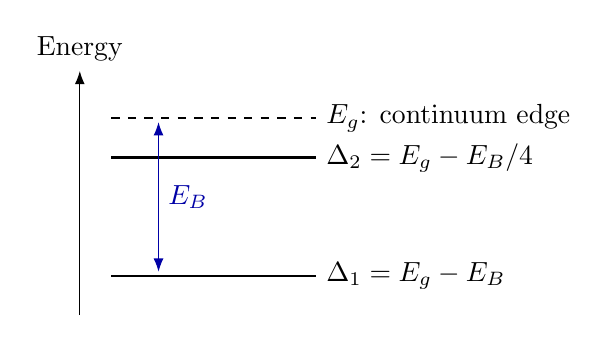
\begin{tikzpicture}[>=Latex]
\draw[->] (0,0)--(0,3.1) node[above] {Energy};
\draw[thick] (.4,.5)--(3,.5) node[right] {$\Delta_1=E_g-E_B$};
\draw[thick] (.4,2)--(3,2) node[right] {$\Delta_2=E_g-E_B/4$};
\draw[thick,dashed] (.4,2.5)--(3,2.5) node[right] {$E_g$: continuum edge};
\draw[<->,blue!65!black] (1,.55)--(1,2.45) node[midway,right] {$E_B$};
\end{tikzpicture}
\end{center}
This inference requires the series assignment and its $1/n^2$ spectrum. Two unrelated optical peaks, different exciton series, or a nonhydrogenic spectrum would not determine $E_g$ and $E_B$ from these two energies alone.

\section*{5. Complete screening is a statement about total charge}
Use the Fourier convention
\[
\rho(\vct q)=\int\dd^3r\,\ee^{-\ii\vct q\cdot\vct r}\rho(\vct r),
\qquad
\rho(\vct r)=\int\frac{\dd^3q}{(2\pi)^3}
\ee^{\ii\vct q\cdot\vct r}\rho(\vct q).
\]
For an external point charge $Ze$ at the origin,
$\rho_{\rm ext}(\vct r)=Ze\delta^{(3)}(\vct r)$ and
$\rho_{\rm ext}(\vct q)=Ze$. In a homogeneous linear dielectric, the screened electrostatic potential is $\phi=\phi_{\rm ext}/\epsilon(q,0)$. Applying Poisson's equation to both potentials gives the same relation for the total charge density:
\[
\rho_{\rm tot}(\vct q)=\frac{Ze}{\epsilon(q,0)},\qquad
\rho_{\rm ind}(\vct q)=Ze\left[\frac1{\epsilon(q,0)}-1\right].
\]
The integrated induced charge is its zero-wavevector component:
\[
Q_{\rm ind}=\int\rho_{\rm ind}(\vct r)\dd^3r
=Ze\left[\lim_{q\to0}\frac1{\epsilon(q,0)}-1\right].
\]
For the stated metallic static limit, the inverse dielectric function tends to zero. Thus
\[
\boxed{Q_{\rm ind}=-Ze,\qquad Q_{\rm ext}+Q_{\rm ind}=0.}
\]
The external charge is completely compensated by the induced screening cloud. This does not mean the local charge or electric field is zero at every point. The argument concerns the static bulk response and its integrated charge; the static limit has already been taken before $q\to0$.

\section*{6. Thomas--Fermi screening and its short-distance defect}
\subsection*{(a) Dielectric function}
The linear Thomas--Fermi approximation replaces the static density response by its long-wavelength value:
\[
\boxed{\epsilon_{\rm TF}(q)=1+\frac{k_{\rm TF}^2}{q^2}.}
\]
In SI units, $k_{\rm TF}^2=(e^2/\varepsilon_0)(\partial n/\partial\mu)$ for the electron gas. A positive compressibility gives $k_{\rm TF}^2>0$. Inserting this expression into the result of Question 5 yields
\[
\rho_{\rm ind}(\vct q)=-Ze\frac{k_{\rm TF}^2}{q^2+k_{\rm TF}^2}.
\]
The minus sign comes directly from $1/\epsilon-1$, which is negative. It must not be inserted a second time in front of that difference.

\subsection*{(b) Fourier inversion and the divergence}
For $r>0$, spherical integration gives
\begin{align*}
\int\frac{\dd^3q}{(2\pi)^3}
\frac{\ee^{\ii\vct q\cdot\vct r}}{q^2+k_{\rm TF}^2}
&=\frac1{2\pi^2r}\int_0^\infty
\frac{q\sin(qr)}{q^2+k_{\rm TF}^2}\dd q\\
&=\frac{\ee^{-k_{\rm TF}r}}{4\pi r}.
\end{align*}
Hence
\[
\boxed{\rho_{\rm ind}(r)=-\frac{Ze k_{\rm TF}^2}{4\pi r}
\ee^{-k_{\rm TF}r}.}
\]
For a positive external charge, the induced electron \emph{number} density is
\[
\boxed{\delta n(r)=-\frac{\rho_{\rm ind}(r)}e
=\frac{Zk_{\rm TF}^2}{4\pi r}\ee^{-k_{\rm TF}r}
\longrightarrow+\infty\quad(r\to0^+).}
\]
The singularity is $1/r$. It is integrable in three dimensions:
\[
\int\rho_{\rm ind}\dd^3r
=-Ze k_{\rm TF}^2\int_0^\infty r\ee^{-k_{\rm TF}r}\dd r
=-Ze.
\]
Thus an infinite local density does not imply an infinite total screening charge. The divergence exposes the failure of extrapolating a linear, long-wavelength response to arbitrarily short distances from a point charge. Atomic structure, nonlocal response, and nonlinear effects are outside that approximation. The supplied answer's final negative induced-charge density is consistent; its intermediate extra minus before $(1/\epsilon-1)$ is not.

\section*{7. Plasmons, energy loss, and causal dispersion relations}
\subsection*{(a) Long-wavelength plasmon branch}
Longitudinal collective modes are zeros of the dielectric function. Multiplying the stated expression by $\omega^4$ gives
\[
\omega^4-\omega_p^2\omega^2-\frac35\omega_p^2v_F^2q^2=0.
\]
Solving the quadratic equation in $x=\omega^2$ and choosing the positive branch connected to $\omega_p$ at $q=0$ yields
\[
\omega^2(q)=\frac{\omega_p^2}{2}
\left[1+\sqrt{1+\frac{12v_F^2q^2}{5\omega_p^2}}\right].
\]
This closed form solves the \emph{truncated} dielectric expression; it does not fix the higher-order terms of the full electron-gas dispersion. Expanding consistently to second order gives
\[
\boxed{\omega^2(q)=\omega_p^2+\frac35v_F^2q^2+O(q^4),}
\]
\[
\boxed{\omega(q)=\omega_p\left[1+\frac3{10}
\frac{v_F^2q^2}{\omega_p^2}+O(q^4)\right].}
\]
The expansion assumes $v_Fq\ll\omega_p$. The other algebraic root has $\omega^2<0$ for $q\ne0$ and lies outside the high-frequency approximation used to obtain the dielectric function; it is not a second physical plasmon branch of this approximation.

\subsection*{(b) Energy-loss function}
For real positive frequency,
\[
\frac1{\epsilon(\omega)}
=\frac{\omega^2+\ii\gamma\omega}
{\omega^2-\omega_p^2+\ii\gamma\omega}.
\]
Multiply numerator and denominator by the complex conjugate of the denominator. The imaginary numerator is
$\gamma\omega(\omega^2-\omega_p^2)-\gamma\omega^3
=-\gamma\omega\omega_p^2$. Therefore
\[
\boxed{L(\omega)=-\operatorname{Im}\frac1{\epsilon(\omega)}
=\frac{\gamma\omega\omega_p^2}
{(\omega^2-\omega_p^2)^2+\gamma^2\omega^2}.}
\]
It is nonnegative for $\omega>0$ and $\gamma>0$. This longitudinal loss function is distinct from $\operatorname{Im}\epsilon$. For weak damping it has a narrow resonance near $\omega_p$; the maximum need not be exactly at $\omega_p$ for finite damping.

\subsection*{(c) Ordinary Kramers--Kronig relations}
Let $\epsilon=\epsilon_1+\ii\epsilon_2$ and assume that $\epsilon(z)-1$ is a causal response analytic in the upper half of the complex frequency plane, decays sufficiently at infinity, and has nonsingular boundary values for the following ordinary-function formulas. With the chosen $\ee^{-\ii\omega t}$ convention,
\begin{align*}
\boxed{\epsilon_1(\omega)-1
=\frac1\pi\operatorname{PV}\int_{-\infty}^{\infty}
\frac{\epsilon_2(\omega')}{\omega'-\omega}\dd\omega',}\\
\boxed{\epsilon_2(\omega)
=-\frac1\pi\operatorname{PV}\int_{-\infty}^{\infty}
\frac{\epsilon_1(\omega')-1}{\omega'-\omega}\dd\omega'.}
\end{align*}
Here PV denotes the Cauchy principal value. For a real time-domain response, $\epsilon_1$ is even and $\epsilon_2$ is odd, giving the equivalent positive-frequency relations
\begin{align*}
\epsilon_1(\omega)-1
&=\frac2\pi\operatorname{PV}\int_0^\infty
\frac{\omega'\epsilon_2(\omega')}{\omega'^2-\omega^2}\dd\omega',\\
\epsilon_2(\omega)
&=-\frac{2\omega}{\pi}\operatorname{PV}\int_0^\infty
\frac{\epsilon_1(\omega')-1}{\omega'^2-\omega^2}\dd\omega'.
\end{align*}
A different high-frequency dielectric background replaces the number 1. Singular conductivity contributions require a subtraction or a distributional treatment, as in part (d).

\subsection*{(d) Drude is causal, but the zero-frequency pole matters}
The analytic continuation of the stated Drude function is
\[
\epsilon(z)=1-\frac{\omega_p^2}{z(z+\ii\gamma)}.
\]
Its poles are at $z=0$ and $z=-\ii\gamma$, not in the open upper half-plane. The pole on the real-axis boundary represents DC conduction. It does \emph{not} by itself make the response acausal. The precise answer is:
\begin{quote}
The Drude dielectric function satisfies causal dispersion relations with the zero-frequency conductivity term treated correctly. Applying the nonsingular ordinary-function formulas from part (c) to its smooth off-zero real and imaginary parts without that term is incomplete.
\end{quote}

To demonstrate the correction, define
\[
K=\frac{\omega_p^2}{\gamma}=\frac{\sigma_{\rm dc}}{\varepsilon_0},\qquad
\epsilon(z)-1=\frac{\ii K}{z}-\frac{\ii K}{z+\ii\gamma}.
\]
Subtract the singular term:
\[
\epsilon_{\rm reg}(z)=\epsilon(z)-\frac{\ii K}{z}
=1-\frac{\ii K}{z+\ii\gamma}.
\]
This regular response obeys the ordinary relations. For real $\omega\ne0$,
\begin{align*}
\epsilon_1(\omega)-1&=-\frac{\omega_p^2}{\omega^2+\gamma^2},\\
\epsilon_2(\omega)&=\frac{\omega_p^2\gamma}{\omega(\omega^2+\gamma^2)},\\
\operatorname{Im}\epsilon_{\rm reg}(\omega)
&=\epsilon_2(\omega)-\frac K\omega
=-\frac{K\omega}{\omega^2+\gamma^2}.
\end{align*}
Restoring the subtracted pole gives, for nonzero observation frequency,
\begin{align*}
\boxed{\epsilon_1(\omega)-1
=\frac2\pi\operatorname{PV}\int_0^\infty
\frac{\omega'\epsilon_2(\omega')}{\omega'^2-\omega^2}\dd\omega',}\\
\boxed{\epsilon_2(\omega)=\frac{K}{\omega}
-\frac{2\omega}{\pi}\operatorname{PV}\int_0^\infty
\frac{\epsilon_1(\omega')-1}{\omega'^2-\omega^2}\dd\omega'.}
\end{align*}
The first relation is unchanged because
$\operatorname{PV}\int_0^\infty\dd\omega'/(\omega'^2-\omega^2)=0$ for $\omega\ne0$. The additional $K/\omega$ in the second is essential. It is also the correction displayed at the end of the supplied answer.

For an explicit check, the ordinary inverse transform of the smooth real part produces
$-K\omega/(\omega^2+\gamma^2)$, not the complete $\epsilon_2$. Adding $K/\omega$ recovers
\[
\frac K\omega-\frac{K\omega}{\omega^2+\gamma^2}
=\frac{K\gamma^2}{\omega(\omega^2+\gamma^2)}
=\frac{\omega_p^2\gamma}{\omega(\omega^2+\gamma^2)}.
\]

\textbf{Equivalent retarded prescription.} The boundary value is approached from $z=\omega+\ii0^+$. The identity
\[
\frac1{\omega+\ii0^+}=\operatorname{PV}\frac1\omega-\ii\pi\delta(\omega)
\]
shows that the complete distributional real part contains
$\pi K\delta(\omega)$ in addition to $1-\omega_p^2/(\omega^2+\gamma^2)$. Keeping this zero-frequency term restores the usual distributional Kramers--Kronig pair. The pole-subtracted formulas above avoid treating the delta function explicitly when $\omega\ne0$.

\textbf{A regulator is not a new physical model.} If ordinary nonsingular boundary values are desired, one can use
\[
\epsilon_\eta(\omega)=1-\frac{\omega_p^2}
{(\omega+\ii\eta)(\omega+\ii\gamma)},\qquad \eta>0,
\]
perform the transforms, and then take $\eta\to0^+$. At any finite $\eta$, both poles are below the real axis and the ordinary relations hold. The limit at zero frequency is nonuniform, which is exactly why the pole term cannot be dropped.

The alternative expression $1-\omega_p^2/(\omega+\ii\gamma/2)^2$ is also causal, but it changes the model: it has finite static permittivity $1+4\omega_p^2/\gamma^2$ and zero DC conductivity. Dropping its $\gamma^2/4$ denominator term is not justified near $\omega=0$. It should not be presented as an equivalent repair of the original conducting Drude response.

\section*{Primary references and verification scope}
The calculations above use the stated models and explicit algebra. The following sources support the conventions and physical distinctions:
\begin{itemize}
\item \href{https://www.nonmet.mat.ethz.ch/education/courses/Materialwissenschaft_1/Downloads_HS_2007/slides_chapter_2.pdf}{ETH Zurich, Material Science I: Crystal Chemistry}, Madelung-constant table: nearest-distance normalization for NaCl and CsCl.
\item \href{https://doi.org/10.1103/PhysRev.166.599}{D. M. Roessler and W. C. Walker, Electronic Spectra of Crystalline NaCl and KCl (1968)}: exciton and interband absorption are distinct spectral features.
\item \href{https://arxiv.org/abs/1003.4724}{V. B. Bobrov, S. A. Trigger, G. J. F. van Heijst, and P. P. J. M. Schram, Kramers--Kronig Relations for the Dielectric Function and the Static Conductivity of Coulomb Systems (2010)}, equations 27--28: the conductivity-pole contribution.
\end{itemize}
The accompanying numerical checks enumerate the Evjen cell, differentiate the pair energy with respect to volume, check spectral formulas, integrate the screening charge, and evaluate the pole-subtracted dispersion relations. These checks verify the displayed model calculations; they do not turn the approximate ionic and screening models into exact material predictions.

\chapter{Solid State Theory: Undated Midterm Fragment}
\label{s:theory-undated-midterm-fragment}
\begin{sourceNote}
Question 2 lacks its defining model. Its numerical answers cannot be recovered uniquely. The conditional method below is an additional study aid, not a claim about the missing original problem. Questions 3--7 can be answered from the surviving text. All band curvatures and density-of-states factors below are derived from the printed dispersion, independently of the handwritten references.
\end{sourceNote}

\section*{2. What can and cannot be inferred}
Band gaps and effective masses depend on the Hamiltonian. Without the potential or the missing model parameters, there is no unique answer to any of the three subparts. In particular, the list of requested quantities does not specify whether the problem uses a nearly-free-electron, tight-binding, or other model.

\textbf{Conditional example: weak one-dimensional periodic potential.}
Suppose, in addition to the surviving text, that one is given
\[
V(x)=\sum_{n\in\mathbb Z}V_{nG}\ee^{\ii nGx},\qquad G=\frac{2\pi}{a},
\qquad V_{-nG}=V_{nG}^*.
\]
At the first free-electron crossing, the waves $k=G/2$ and $k-G=-G/2$ are coupled by $V_G$. Their $2\times2$ Hamiltonian has equal diagonal terms at the crossing and off-diagonal terms $V_G,V_G^*$, so the leading first gap is
\[
\Delta_1\simeq2|V_G|.
\]
The crossing of $+G$ and $-G$ involves $V_{2G}$, hence the leading direct second gap is $\Delta_2\simeq2|V_{2G}|$. If a Fourier coefficient vanishes, a higher-order effective coupling can still open a gap. A zero first-order expression is not proof of an exact zero gap.

For the first crossing let $k=G/2+q$, $B=\hbar^2/(2m)$, $K=G/2$, and $v=|V_G|>0$. Diagonalizing the two-wave matrix gives
\[
E_\pm(q)=V_0+B(K^2+q^2)\pm\sqrt{v^2+4B^2K^2q^2}.
\]
Expanding the lower branch at $q=0$,
\[
E_-(q)=V_0+BK^2-v+
\left(B-\frac{2B^2K^2}{v}\right)q^2+O(q^4),
\]
so the electron curvature mass obeys
\[
\boxed{\frac1{m^*}=\frac1{\hbar^2}E_-''(0)
=\frac1m-\frac{\hbar^2G^2}{4m^2|V_G|}.}
\]
For a weak potential the curvature is negative, as expected at the top of the lower band; the corresponding hole mass is positive. These formulas require an isolated weak-potential crossing and are not numerical answers to the cropped question.

\section*{3. One-orbital nearest-neighbor chain}
Take orthonormal localized orbitals $\ket n$ at $x=na$, on-site matrix element $\epsilon_0$, and real nearest-neighbor hopping $\gamma<0$:
\[
H=\epsilon_0\sum_n\ket n\bra n+
\gamma\sum_n\bigl(\ket n\bra{n+1}+\ket{n+1}\bra n\bigr).
\]
The Bloch state is $\ket k=N^{-1/2}\sum_n\ee^{\ii kna}\ket n$. Acting with $H$ and relabelling the two hopping sums yields
\[
H\ket k=[\epsilon_0+\gamma\ee^{\ii ka}+\gamma\ee^{-\ii ka}]\ket k,
\qquad E(k)=\epsilon_0+2\gamma\cos ka.
\]
Since $E(0)=\epsilon_0+2\gamma$,
\[
\boxed{E(k)=E(0)+2\gamma(\cos ka-1).}
\]
For $\gamma<0$, $k=0$ is a minimum, $k=\pi/a$ is a maximum, and the bandwidth is $4|\gamma|$. Near the minimum, $E(k)=E(0)-\gamma a^2k^2+O(k^4)$, giving $m^*=-\hbar^2/(2\gamma a^2)>0$.

The printed phrase ``inter-orbital overlap'' must mean the hopping \emph{energy} here. A dimensionless nonorthogonal overlap $s=\braket n{n+1}$ would instead lead to a generalized eigenproblem and, in the analogous nearest-neighbor model, $E(k)=(\epsilon_0+2\gamma\cos ka)/(1+2s\cos ka)$.

\section*{4. True or false}
\textbf{(a) False.} A crystal can have multiple identical atoms in its basis. Diamond has an FCC Bravais lattice with two identical atoms at $0$ and $a(1,1,1)/4$. Their difference is not an FCC lattice vector. Translating by that displacement does not map the whole diamond lattice onto itself. Identical chemical species therefore need not be translation-equivalent basis sites.

\textbf{(b) True for a point strictly outside the first zone.} By definition the first Brillouin zone is the reciprocal-space Wigner--Seitz cell
\[
\mathcal B_1=\{\vct k:|\vct k|\le|\vct k-\vct G|
\text{ for every reciprocal vector }\vct G\}.
\]
Failure to belong to this closed cell means that some nonzero $\vct G$ satisfies $|\vct k-\vct G|<|\vct k|$. On a zone boundary equality can occur; the statement's strict comparison concerns points outside, not boundary points.

\section*{5. FCC planes and planar density}
The primitive-cell volume and reciprocal vectors are
\begin{align*}
\Omega&=\vct t_1\cdot(\vct t_2\times\vct t_3)=a^3/4,\\
\vct g_1&=\frac{2\pi}{a}(-1,1,1),\quad
\vct g_2=\frac{2\pi}{a}(1,-1,1),\quad
\vct g_3=\frac{2\pi}{a}(1,1,-1).
\end{align*}
They satisfy $\vct t_i\cdot\vct g_j=2\pi\delta_{ij}$.

\textbf{(a) First direction.} The stated normal is only a direction; its half-integer coefficients do not make it a reciprocal lattice vector. The shortest nonzero reciprocal vector in this direction is
\[
\vct G_0=\vct g_1+2\vct g_2-2\vct g_3
=\frac{2\pi}{a}(-1,-3,5).
\]
The integer triple $(1,2,-2)$ is primitive. For $\vct R=n_1\vct t_1+n_2\vct t_2+n_3\vct t_3$, the plane index is $n_1+2n_2-2n_3$, which runs through every integer. Hence successive occupied planes obey $\vct G_0\cdot\vct R=2\pi\ell$, and
\[
\boxed{d=\frac{2\pi}{|\vct G_0|}=\frac a{\sqrt{35}}.}
\]
Using $2\pi$ divided by the length of the original half-vector would incorrectly skip every other occupied plane.

\textbf{(b) Density.} There is one point per primitive volume, so the volume density is $1/\Omega=4/a^3$. Dividing space into layers separated by $d$ gives
\[
\boxed{\rho_{2D}=\frac d\Omega=\frac4{a^2\sqrt{35}}.}
\]
An independent check is the in-plane primitive basis
\[
\vct u=-2\vct t_1+\vct t_2,\qquad
\vct v=2\vct t_1+\vct t_3.
\]
Every integer solution of $n_1+2n_2-2n_3=0$ is an integer combination of these vectors. Their cell area is $|\vct u\times\vct v|=a^2\sqrt{35}/4$, confirming the reciprocal density.

\textbf{(c) Direct-space normal.} Here
\[
\vct t_1+2\vct t_2-2\vct t_3=\frac a2(0,-1,3).
\]
The shortest reciprocal vector along this direction is
\[
\vct G_1=2\vct g_1+3\vct g_2-\vct g_3
=\frac{2\pi}{a}(0,-2,6).
\]
Its primitive integer coefficients $(2,3,-1)$ show that no shorter collinear reciprocal vector is allowed. Thus
\[
\boxed{d_1=\frac a{\sqrt{40}}=\frac a{2\sqrt{10}}.}
\]
The vector $(2\pi/a)(0,-1,3)$ has mixed odd/even Cartesian indices and is not a reciprocal vector of FCC.

\section*{6. Honeycomb critical points and density of states}
Set $S(\vct k)=|F_{\vct k}|^2$ and $E_\pm=\varepsilon_p\pm\gamma\sqrt S$. Away from $S=0$,
\[
\nabla E_\pm=\pm\frac{\gamma}{2\sqrt S}\nabla S.
\]
One must not apply this quotient at a zero of $S$ without a local expansion.

\textbf{(a) Classification.} At $\Gamma$, expanding both cosines gives
\[
S(\vct q)=9-\frac{3a^2}{2}(q_x^2+q_y^2)+O(q^4),\qquad
|F|=3-\frac{a^2}{4}(q_x^2+q_y^2)+O(q^4).
\]
Therefore
\[
E_\pm(\Gamma+\vct q)=\varepsilon_p\pm3\gamma
\mp\frac{\gamma a^2}{4}(q_x^2+q_y^2)+O(q^4).
\]
Both bands have zero gradient. The lower band has a minimum ($M_0$); the upper band has a maximum ($M_2$), where the Morse index counts negative Hessian eigenvalues.

At $Q=(\pi/a,\pi/(\sqrt3a))$, write $\vct k=Q+\vct q$. The cosine factors vanish at $Q$, and direct expansion yields
\[
S=1+a^2q_x^2+\sqrt3a^2q_xq_y+O(q^4),\qquad
|F|=1+\frac{a^2}{2}q_x^2+\frac{\sqrt3a^2}{2}q_xq_y+O(q^4).
\]
Consequently the Hessian of $|F|$ is
\[
H_{|F|}=a^2\begin{pmatrix}1&\sqrt3/2\\\sqrt3/2&0\end{pmatrix},
\qquad\lambda=\frac{3a^2}{2},\ -\frac{a^2}{2}.
\]
In orthonormal principal coordinates $(u,v)$ this becomes
\[
E_\pm(Q+\vct q)=\varepsilon_p\pm\gamma
\pm\frac{\gamma a^2}{4}(3u^2-v^2)+O(q^4).
\]
Thus both bands have an $M_1$ saddle. The mixed derivative is essential; the trace of the Hessian alone cannot distinguish a saddle from an extremum.

At $P=(4\pi/(3a),0)$, $S(P)=0$. Expanding $S$ gives
\[
S(P+\vct q)=\frac{3a^2}{4}|\vct q|^2+O(|q|^3),\qquad
E_\pm=\varepsilon_p\pm c|\vct q|+O(q^2),\quad c=\frac{\sqrt3\gamma a}{2}.
\]
This is a Dirac contact. Each energy-ordered branch has a conical cusp, so its gradient is undefined exactly at the contact. It is not an ordinary differentiable stationary point of Morse type. The directional slopes are finite and direction-dependent; an infinite gradient inferred by manipulating $0/0$ is incorrect. The direct band gap there is zero.

\begin{center}
\begin{tabular}{llll}
\toprule
Point & $|F|$ & Lower band & Upper band\\
\midrule
$\Gamma$ & 3 & Minimum, $M_0$ & Maximum, $M_2$\\
$Q$ & 1 & Saddle, $M_1$ & Saddle, $M_1$\\
$P$ & 0 & Dirac contact & Dirac contact\\
\bottomrule
\end{tabular}
\end{center}

\textbf{(b) Choose the lower-band minimum at $\Gamma$.}
Let $E_0=\varepsilon_p-3\gamma$ and $\alpha=\gamma a^2/4$. Define the DOS per physical area, including $g_s$ spin states, by
\[
\frac{D(E)}A=\frac{g_s}{(2\pi)^2}\int\dd^2q\,
\delta(E-E_0-\alpha q^2).
\]
For an energy close enough to the edge that the contour stays in the chosen neighborhood,
\begin{align*}
\frac{D_\Gamma(E)}A
&=\frac{g_s}{(2\pi)^2}\,2\pi\int_0^\infty q\dd q\,
\delta(E-E_0-\alpha q^2)\\
&=\frac{g_s}{4\pi\alpha}\Theta(E-E_0)
=\boxed{\frac{g_s}{\pi\gamma a^2}\Theta(E-E_0)}.
\end{align*}
For spin degeneracy two, this is $2/(\pi\gamma a^2)$ above the edge and zero below. The total DOS is this result multiplied by area $A$. Near the upper-band maximum $E_2=\varepsilon_p+3\gamma$, the same coefficient multiplies $\Theta(E_2-E)$. These are local edge formulas, not constants throughout the full band.

For comparison, one Dirac valley has
\[
\frac{D_P(E)}A=\frac{g_s|E-\varepsilon_p|}{2\pi c^2}
=\frac{2g_s|E-\varepsilon_p|}{3\pi\gamma^2a^2}.
\]
Counting both inequivalent valleys adds a factor of two; one must not count six full independent valleys merely because the hexagonal zone has six corners. A saddle at $Q$ gives a logarithmic local singularity. With $A_q=3\gamma a^2/4$ and $B_q=\gamma a^2/4$, its leading form per saddle and per band is
\[
\frac{D_Q(E)}A\sim\frac{g_s}{4\pi^2\sqrt{A_qB_q}}
\log\frac{E_c}{|E-E_Q|},
\]
where the cutoff $E_c$ depends on the chosen neighborhood. A two-dimensional saddle is not described by the step function of a quadratic minimum.

\section*{7. Bloch theorem and its meaning}
For a one-electron Hamiltonian with a Bravais-periodic potential,
\[
V(\vct r+\vct R)=V(\vct r),
\]
the lattice-translation operators commute with the Hamiltonian and with one another. The eigenstates can be chosen to be simultaneous translation eigenstates:
\[
\psi_{n\vct k}(\vct r+\vct R)=\ee^{\ii\vct k\cdot\vct R}
\psi_{n\vct k}(\vct r).
\]
Writing $u_{n\vct k}(\vct r)=\ee^{-\ii\vct k\cdot\vct r}\psi_{n\vct k}(\vct r)$ then gives
\[
\boxed{\psi_{n\vct k}(\vct r)=\ee^{\ii\vct k\cdot\vct r}u_{n\vct k}(\vct r),
\qquad u_{n\vct k}(\vct r+\vct R)=u_{n\vct k}(\vct r).}
\]
The label $\vct k$ is defined modulo a reciprocal lattice vector and may be restricted to the first Brillouin zone. Bloch's theorem does not assert that the full wavefunction is lattice-periodic, nor that the electron is a free particle; the periodic factor encodes the crystal potential.

\end{document}
